% ==============================================================================
% Manuscript in LaTeX Format (Single-Pass Compilable .tex)
% Title: When Does Jump-Risk Filtering Matter for Commodity Derivatives Deep
%        Hedging? A Semi-Synthetic Simulation Audit of Jump-Modulated No-Trade
%        Bands, Price-Limit Locks, and Option-Gamma Spanning
% Open-source code repository: https://github.com/lewygoat/Jump-Risk-Filtering-Deep-Hedging
% ==============================================================================

\documentclass[11pt,a4paper]{article}

\usepackage[utf8]{inputenc}
\usepackage[T1]{fontenc}
\usepackage[margin=1in]{geometry}
\usepackage{amsmath,amssymb,amsfonts,mathtools}
\usepackage{booktabs,multirow,array,threeparttable}
\usepackage{graphicx}
\usepackage{caption}
\usepackage{xcolor}
\usepackage[numbers,sort&compress]{natbib}
\usepackage[colorlinks=true,linkcolor=blue!70!black,citecolor=blue!70!black,urlcolor=blue!70!black]{hyperref}

\captionsetup{font=small,labelfont=bf}
\setlength{\parskip}{0.35em}
\setlength{\emergencystretch}{2.5em}
\renewcommand{\arraystretch}{1.15}

\title{\textbf{When Does Jump-Risk Filtering Matter for Commodity Derivatives Deep Hedging? A Semi-Synthetic Simulation Audit of Jump-Modulated No-Trade Bands, Price-Limit Locks, and Option-Gamma Spanning}}

\author{
  Anonymous Authors\\[0.3em]
  \small Quantitative Finance \& Derivatives Microstructure Research Group\\
  \small Open-Source Code \& Audit Repository: \url{https://github.com/lewygoat/Jump-Risk-Filtering-Deep-Hedging}
}

\date{\today}

\begin{document}

\maketitle

\begin{abstract}
\noindent
Strategic commodity futures such as Lithium Carbonate (\texttt{LC}) on the Guangzhou Futures Exchange (GFEX) exhibit self-exciting jump clustering alongside daily price-limit bands ($\pm 7\%$ to $\pm 15\%$) that freeze order-book execution upon limit locks. Using a protocol-specified semi-synthetic simulation audit ($80$ single-instrument Deep Hedging checkpoints, $60$ Distributional Actor-Critic \texttt{D4PG-QR} runs, and $80$ two-instrument Option-Gamma checkpoints across $100,000$ S4 benchmark and $20,000$ S5 stress paths), we examine when causal threshold-Hawkes intensity filtering ($\hat{\lambda}_t$) and price-limit features improve Conditional Value-at-Risk ($\text{CVaR}_{95}$) hedging. First, in futures-only hedging ($c = 10^{-4}$), CVaR-trained Deep Hedging (\texttt{DH1}, $\text{CVaR}_{95} = 0.021078 \pm 0.000105$) reduces tail loss by $27.00\%$ versus Black-76 delta hedging ($0.028872$) and by $32.64\%$ versus mean-variance hedging (\texttt{DH\_mv}, $0.031294$, $p_{\text{holm}} = 3.9 \times 10^{-11}$), dominating mean-variance across $\lambda_{\text{MV}} \in [0.5, 50.0]$ while avoiding the $20\%\text{--}30\%$ seed collapse rate of \texttt{D4PG-QR}. Second, embedding $\hat{\lambda}_t$ into a multiplicative no-trade band (\texttt{DH\_lband}, \texttt{DH\_full}) yields a negative modulation slope ($\hat{\theta} = -0.0276, p = 0.0019$; $\hat{\theta} = -0.0230, p = 0.0011$) that contracts the buffer during jump bursts, cutting trading frequency by $20.11\%$, transaction costs by $8.09\%$, and the lock-step hedging gap (\texttt{LockGap}) by $29.65\%$ on S4 and $25.67\%$ on S5 (where \texttt{DH\_full} reduces $\text{CVaR}_{95}$ by $37.60\%$ vs.\ \texttt{B76-Delta} as drift-neutralized tail risk rises $+17.89\%$), with no statistically detectable $\text{CVaR}_{95}$ degradation relative to \texttt{DH1} at $6\times$ cost ($p = 0.218, p_{\text{TOST}} = 0.046$). Third, Jacobian saliency ($>99.78\%$ on core states) and oracle tests (\texttt{DH\_oracle}, $0.021085$) show that linear futures ($\Gamma^{\text{fut}} = 0$) face a spanning ceiling. Adding a rolling 20-day ATM call option breaks this ceiling ($-17.98\%$ to $-29.95\%$), and channeling $\hat{\lambda}_t$ through the structural no-trade band (\texttt{DH\_opt\_lband}, $\hat{\theta} = -0.0290, p = 1.59 \times 10^{-7}$) achieves the lowest 2D $\text{CVaR}_{95}$ of $0.014841 \pm 0.001316$ ($+15.41\%$ vs.\ \texttt{DH\_opt\_cband}, $p_{\text{holm}} = 0.000123$). Code is available at \url{https://github.com/lewygoat/Jump-Risk-Filtering-Deep-Hedging}.

\vspace{0.6em}
\noindent\textbf{Keywords:} Deep Hedging; Hawkes Jump Process; Online Intensity Filtering; Price-Limit Microstructure; Conditional Value-at-Risk (CVaR); Multi-Instrument Gamma Hedging; Lithium Carbonate Futures\\[0.3em]
\noindent\textbf{JEL Classification:} G13; G11; C45; C61; Q02
\end{abstract}

% ==============================================================================
% SECTION 1: INTRODUCTION AND RELATED WORK
% ==============================================================================
\section{Introduction and Related Work}
\label{sec:intro}

\subsection{Background and Research Motivation}
The expansion of global green-energy supply chains has made strategic battery metals---such as Lithium Carbonate (\texttt{LC}) futures launched on the Guangzhou Futures Exchange (GFEX) in July 2023---important instruments for industrial risk management in the lithium value chain \citep{Kong2024,Wang2025}, alongside broader clean-energy and commodity futures markets \citep{Coskun2023}. Unlike frictionless geometric Brownian diffusion \citep{Black1976}, emerging strategic commodity futures in China exhibit two major microstructural departures documented across domestic energy, agricultural, and metal futures markets \citep{Naqvi2023,Geng2025}. First, supply-chain bottlenecks, inventory squeezes, and policy announcements generate abrupt price discontinuities \citep{Merton1976,Kou2002} that cluster in time, a self-exciting dynamic captured by Hawkes point processes \citep{Hawkes1971,Bacry2015,Brignone2023} and marked jump-clustering specifications \citep{ChenClements2024,Mercuri2024}. Second, Chinese commodity futures exchanges enforce statutory daily price-limit bands ($\pm 7\%$ to $\pm 15\%$ on GFEX \texttt{LC}) accompanied by directional order-book locks when prices reach the boundary, analogous to price-limit execution freezes and volatility spillover effects examined in equity and agricultural futures markets \citep{KimRhee1997,Zhang2023,Xia2024}. During a limit lock, one-sided liquidity vanishes, freezing a hedger's ability to rebalance a short option liability when underlying Gamma convexity losses are largest.

Classical analytical hedging rules---including \citet{Black1976} practitioner delta (\texttt{B76-Delta}), discrete-time delta rebalancing \citep{BoyleEmanuel1980,Bakshi1997}, \citet{Leland1985} volatility-adjusted delta (\texttt{Leland-Delta}), and \citet{Whalley1997} asymptotic no-trade bands (\texttt{WW-Band})---rely on local diffusive Taylor expansions and continuous trade execution. As a result, their hedging performance degrades under jump clustering and execution freezes \citep{Merton1976,Jouini2026,Shakeel2026}. Introduced by \citet{Buehler2019}, \textbf{Deep Hedging (DH)} formulates derivative hedging as an end-to-end neural network control problem under convex risk measures such as Conditional Value-at-Risk ($\text{CVaR}$, \citealt{Rockafellar2000}). Subsequent work has extended Deep Hedging to long-term derivatives \citep{Carbonneau2021}, rough volatility \citep{Horvath2021}, quadratic hedging benchmarks \citep{Dai2022}, parameter ambiguity \citep{Luetkebohmert2022}, equal risk pricing \citep{Marzban2022,CarbonneauGodin2024}, empirical equity index options \citep{Mikkila2023,Francois2025}, neural no-transaction band networks \citep{Imaki2023}, signature volatility models \citep{AbiJaber2025}, backward dynamic programming with transaction costs \citep{Goudenege2023,Brugiere2026}, and model-free distributional reinforcement learning (\texttt{D4PG-QR}, \citealt{Cao2023,Pickard2023}).

Despite this progress, a clear research gap remains at the intersection of self-exciting jump filtering and emerging-market institutional trading frictions. Specifically, three questions remain open:
\begin{enumerate}
  \item \textbf{When and through which architectural channel does online jump-intensity filtering matter ($\mathbf{H_0, H_1}$)?} Does feeding a causal threshold-Hawkes jump-intensity proxy $\hat{\lambda}_t$ into a deep hedging policy reduce tail risk when hedging solely with linear futures, or does it require a second, convex option instrument ($\Gamma > 0$) and a structural no-trade band parameterization to extract \emph{ex-ante} jump-Gamma protection without optimization variance?
  \item \textbf{How do jump intensity and price limits reshape microstructural trading rules ($\mathbf{H_1, H_3}$)?} Can a neural policy learn without sign constraints to modulate its no-trade band width $w_t(x_t)$ in response to $\hat{\lambda}_t$ and pre-position its hedge ratio ahead of price-limit locks?
  \item \textbf{How do risk objectives ($\mathbf{H_2}$) and optimization methods (\texttt{BPTT} vs.\ \texttt{D4PG-QR}) interact with these frictions?} Does symmetric mean-variance hedging or model-free distributional reinforcement learning remain effective under self-exciting jumps and price-limit truncations?
\end{enumerate}

\subsection{Related Literature}
Our study relates to three strands of the quantitative finance literature:

\paragraph{1. Deep Hedging and Convex Risk Optimization Under Market Frictions.}
Classical option replication under discrete rebalancing \citep{BoyleEmanuel1980}, jump-diffusion return discontinuities \citep{Merton1976,Bakshi1997}, and proportional transaction costs \citep{Leland1985,Whalley1997} established that market incompleteness and trading frictions prevent exact delta replication. \citet{Buehler2019} established Deep Hedging via end-to-end Back-Propagation Through Time (BPTT) under proportional transaction costs and convex risk measures \citep{Rockafellar2000}. \citet{Carbonneau2021} and \citet{Dai2022} evaluated neural networks for long-term and quadratic hedging, while \citet{Horvath2021} and \citet{Luetkebohmert2022} studied rough volatility and parameter ambiguity. \citet{Marzban2022} and \citet{CarbonneauGodin2024} formulated equal-risk pricing and hedging across single and multiple hedging instruments. Empirically and architecturally, \citet{Mikkila2023} and \citet{Francois2025} showed that deep hedging outperforms practitioner delta hedging on equity index options, \citet{NaWan2023} and \citet{Goudenege2023} developed recurrent and backward hedging schemes for American options with transaction costs, and \citet{Imaki2023} and \citet{Babaei2024} analyzed no-transaction band networks and fixed-plus-proportional cost buffers. \citet{AbiJaber2025} and \citet{Brugiere2026} studied signature volatility models and data-augmented model-free deep hedging, while \citet{Shakeel2026} examined neural SDE hedging under regime-switching jump diffusions. To the best of our knowledge, none of these studies incorporate exchange price-limit locks or identify the spanning and architectural boundary between linear futures hedging and multi-instrument Gamma hedging under Hawkes jumps.

\paragraph{2. Distributional Reinforcement Learning for Option Greek Hedging.}
Building on quantile regression distributional reinforcement learning (\texttt{QR-DQN}, \citealt{Dabney2018}), \citet{Cao2023} applied Distributional Deep Deterministic Policy Gradient (\texttt{D4PG-QR}) to hedge option Gamma and Vega under transaction costs, an approach reviewed by \citet{Pickard2023} and extended to shortfall-aware implied-volatility hedging by \citet{ChenHu2026}. While \texttt{D4PG-QR} avoids differentiating through the market simulator, its reliance on off-policy multi-step quantile Bellman bootstrapping has not been tested against direct pathwise BPTT in finite-horizon commodity markets with self-exciting jump clusters and price-limit truncations.

\paragraph{3. Jump Clustering and Institutional Price Limits in Commodity Futures.}
Recent studies document pronounced tail risk, volatility asymmetry, and cross-market spillovers in China's lithium carbonate industry chain \citep{Kong2024,Wang2025}, clean-energy equity--commodity portfolios \citep{Coskun2023}, and Chinese crude oil futures \citep{Naqvi2023,Geng2025}. To model contagious price shocks in financial and commodity markets \citep{AitSahalia2015,Bacry2015}, \citet{Brignone2023} and \citet{Mercuri2024} developed option pricing models with jump clusters and compound CARMA-Hawkes processes, while \citet{ChenClements2024} and \citet{deTruchis2025} modeled marked Hawkes jump clustering and fractional volatility persistence. \citet{Qiao2025} and \citet{HeYan2026} analyzed jump components and self-exciting jumps in volatility forecasting and variance swap valuation. In addition, \citet{He2026} and \citet{Jouini2026} studied jump volatility forecasting and crisis-regime dynamic hedging, while \citet{KimRhee1997}, \citet{Zhang2023}, and \citet{Xia2024} examined price-limit execution frictions, asymmetric risk connectedness, and session volatility in Asian equity and Chinese agricultural/energy futures markets. Combining causal online Hawkes filtering with institutional price-limit execution freezes for dynamic derivative hedging remains unexplored.

\subsection{Summary of Contributions}
Evaluating $80$ formal 1D Deep Hedging (\texttt{DH}) checkpoints, $60$ \texttt{D4PG-QR} runs, and $80$ formal 2D Option-Gamma checkpoints across 10 random seeds (\texttt{9001--9010}) on $100,000$ S4 benchmark paths and $20,000$ S5 extreme stress paths in a controlled semi-synthetic environment partially calibrated to GFEX Lithium Carbonate (\texttt{LC}) futures, we make four calibrated contributions:

\begin{itemize}
  \item \textbf{Contribution 1 (Asymmetric CVaR Dominance in $(\text{CVaR}_{95}, \text{Cost})$ over Baselines and Mean-Variance, $\mathbf{H_2}$):}
  Under the S4 futures-only benchmark ($100,000$ paths, $c = 10^{-4}$), relative to classical Black-76 delta hedging (\texttt{B76-Delta}) and symmetric mean-variance deep hedging (\texttt{DH\_mv}, $\lambda_{\text{MV}}=10$), our CVaR-trained policy (\texttt{DH1}) improves out-of-sample $\text{CVaR}_{95}$ from $0.028872$ (\texttt{B76-Delta}) and $0.031294 \pm 0.000722$ (\texttt{DH\_mv}) to $0.021078 \pm 0.000105$ ($p_{\text{holm}} = 3.9 \times 10^{-11}$) while reducing transaction costs from $0.5015 \times 10^{-3}$ (\texttt{DH\_mv}) to $0.3166 \times 10^{-3}$ and dominating \texttt{DH\_mv} in the $(\text{CVaR}_{95}, \text{Cost})$ plane across $\lambda_{\text{MV}} \in [0.5, 50.0]$, at the cost of a higher loss standard deviation $\text{Std}(L)$ ($0.013391$ in \texttt{DH1} vs.\ $0.012539$ in 10-seed \texttt{DH\_mv} at $\lambda_{\text{MV}}=10$ and $0.012798$ at $\lambda_{\text{MV}}=50$) because asymmetric $\text{CVaR}_{95}$ leaves upside convex hedging gains ($L_T < 0$) unpenalized.

  \item \textbf{Contribution 2 (Jump-Modulated No-Trade Band and Price-Limit Pre-Positioning, $\mathbf{H_1}$ \& $\mathbf{H_3}$):}
  Under the S4 benchmark ($100,000$ paths) and the S5 extreme stress regime ($20,000$ paths), relative to the static-band policy (\texttt{DH\_cband}) and unconstrained policy (\texttt{DH1}), our Hawkes-modulated band (\texttt{DH\_lband}) and full microstructure-aware policy (\texttt{DH\_full}) improve S4 $\text{CVaR}_{95}$ from $0.021512 \pm 0.000133$ (\texttt{DH\_cband}) to $0.021187 \pm 0.000183$ ($p_{\text{holm}} = 0.00063$, a statistically significant microstructural adaptation with modest $+1.51\%$ 1D magnitude), reduce S4 trading frequency from $99.95\%$ (\texttt{DH1}) to $79.85\%$ and transaction costs from $0.3166 \times 10^{-3}$ to $0.2910 \times 10^{-3}$, compress the cumulative lock-step hedging gap (\texttt{LockGap}) from $0.935 \times 10^{-2}$ (\texttt{DH1}) to $0.658 \times 10^{-2}$ (\texttt{DH\_full}, $-29.65\%$) on S4 and from $2.162 \times 10^{-2}$ to $1.607 \times 10^{-2}$ ($-25.67\%$) on S5, and exhibit no statistically detectable $\text{CVaR}_{95}$ degradation relative to unconstrained \texttt{DH1} under zero-shot $6\times$ transaction costs ($0.023145$ vs.\ $0.023241$, $p = 0.218$; $\pm 1\%$ two-one-sided equivalence $p_{\text{TOST}} = 0.046$) while saving $8.11\%$ in friction, at the cost of a $0.52\%$ higher $\text{CVaR}_{95}$ on low-cost $1\times$ S4 ($0.021187 > 0.021078$) where the $2.56 \times 10^{-5}$ fee savings are smaller than the band-induced tracking error.

  \item \textbf{Contribution 3 (Option-Gamma Spanning and Structural Band Activation of Jump Filtering, $\mathbf{H_0, H_1, H_2}$):}
  Under the 10-seed two-instrument futures-and-rolling-ATM-option hedging environment (\texttt{TorchHedgeEnvOpt}, $\tau_h = 20$ days) on S4, relative to 1D futures policies (\texttt{DH1} $0.021078$, \texttt{DH\_lband} $0.021187$) and 2D static-band hedging (\texttt{DH\_opt\_cband} $0.017546 \pm 0.002298$), adding the option leg reduces $\text{CVaR}_{95}$ by $17.98\%\text{--}29.95\%$ across all 2D configurations, while embedding $\hat{\lambda}_t$ into the multiplicative no-trade band (\texttt{DH\_opt\_lband}, $\hat{\theta} = -0.0290 \pm 0.0064, p = 1.59 \times 10^{-7}$) achieves the lowest realistic 2D $\text{CVaR}_{95}$ of $0.014841 \pm 0.001316$ ($+15.41\%$ vs.\ \texttt{DH\_opt\_cband}, $t = -7.401, p_{\text{holm}} = 0.000123$; $-29.95\%$ vs.\ 1D \texttt{DH\_lband}), at the cost of requiring a liquid short-dated option market, whereas feeding $\hat{\lambda}_t$ into an unconstrained 2D MLP (\texttt{DH\_opt1}, $0.015226 \pm 0.001497$) yields an $11.91\%$ 10-seed point improvement over \texttt{DH\_opt\_nolam} ($0.017284 \pm 0.004298$, $p_{\text{holm}} = 0.450$; $+21.56\%$ in the 5-seed subset) that does not achieve standalone statistical significance due to cross-seed non-convex optimization variance and information overlap with nonlinear $\sigma_{\text{EWMA}}$ features (\texttt{DH\_opt\_ewma\_nl}, $0.015904$) and attenuates from $+11.91\%$ to $+5.31\%$ ($\kappa_{\text{iv}}=2$) and $+0.73\%$ ($\kappa_{\text{iv}}=5$) when option implied volatility co-jumps with $\hat{\lambda}_t$.

  \item \textbf{Contribution 4 (Optimization Stability of Direct BPTT over Distributional RL):}
  Under the 10-seed formal benchmark on S4 across training budgets of $3,000$ to $20,000$ updates, relative to model-free Distributional Actor-Critic with Quantile Regression (\texttt{D4PG-QR (C1)}), end-to-end differentiable \texttt{DH1} (BPTT) improves all-seed $\text{CVaR}_{95}$ from $0.144200 \pm 0.242296$ (and non-collapsed seed mean $0.038934 \pm 0.020739$) to $0.021078 \pm 0.000105$ while reducing the seed collapse rate from $20.0\%\text{--}30.0\%$ to $0.0\%$ ($0/80$ runs) and cross-seed coefficient of variation from $50.02\%$ to $0.50\%$ ($0.09\%$ at $20,000$ updates), at the cost of requiring an explicitly known, piecewise-differentiable market transition and accounting simulator rather than purely model-free interaction.
\end{itemize}

% ==============================================================================
% SECTION 2: MARKET MICROSTRUCTURE MODEL AND ONLINE HAWKES JUMP FILTERING
% ==============================================================================
\section{Market Microstructure Model and Online Hawkes Jump Filtering}
\label{sec:market_model}

\subsection{Underlying Futures Dynamics with Self-Exciting Hawkes Jumps}
We consider a discrete-time commodity futures market indexed by trading days $t \in \{0, 1, \dots, T\}$, partially calibrated to the daily settlement prices of Lithium Carbonate (\texttt{LC}) futures on the Guangzhou Futures Exchange (GFEX) \citep{Kong2024,Wang2025}. Let $F_t > 0$ denote the futures price at day $t$, normalized to $F_0 = 1.0$. Without price-limit truncations, the latent log-return $r_{t+1}^* = \ln(F_{t+1}^* / F_t)$ follows a discrete-time jump-diffusion process driven by a self-exciting Hawkes counting process \citep{Hawkes1971,AitSahalia2015,Bacry2015}:
\begin{equation}
  r_{t+1}^* = \left(\mu_d - \frac{1}{2}\sigma^2 - \lambda_t \bar{k}\right)\Delta t + \sigma \sqrt{\Delta t}\,\varepsilon_{t+1} + \sum_{j=1}^{N_{t+1}} J_{t+1,j}, \quad \varepsilon_{t+1} \stackrel{\text{i.i.d.}}{\sim} \mathcal{N}(0, 1),
  \label{eq:unconstrained_return}
\end{equation}
where $\Delta t = 1$ trading day, $\sigma = 0.016144$ ($0.0161\text{ day}^{-1/2}$, $25.63\%$ annualized) is the $5\%$-trimmed diffusive daily volatility estimated from $534$ non-roll GFEX \texttt{LC} return observations, and $\mu_d = 0$ under the martingale futures measure with jump compensator $\bar{k} = \mathbb{E}[e^{J} - 1]$ \citep{Black1976,Merton1976}.

To capture shock clustering in energy-transition commodity markets \citep{Brignone2023,Mercuri2024} and derivative variance dynamics \citep{deTruchis2025,HeYan2026}, the daily jump count $N_{t+1} \mid \lambda_t \sim \text{Poisson}(\lambda_t)$ obeys the discrete-time Hawkes recursion \citep{Hawkes1971,ChenClements2024}:
\begin{equation}
  \lambda_t - \mu = e^{-\beta}(\lambda_{t-1} - \mu) + \alpha N_t, \quad \lambda_{-300} = \mu,
  \label{eq:hawkes_recursion}
\end{equation}
where $\mu > 0$ is the baseline intensity, $\beta > 0$ is the exponential decay rate, and $\alpha \ge 0$ is the self-excitation magnitude. In our open-source simulator (\texttt{src/simulator.py} and \texttt{src/trainer.py}, publicly available at \url{https://github.com/lewygoat/Jump-Risk-Filtering-Deep-Hedging}), each trajectory is preceded by a $\text{burn\_in} = 300$-step warm-up ($300\beta = 60$ relaxation lifetimes) so that $\lambda_0$ starts from its stationary ergodic distribution rather than a deterministic cold start at $\mu$; the simulator generates $T_{\text{sim}} = 61$ steps to span the $T = 60$-day option hedging horizon plus a one-step terminal index buffer. The stationary branching ratio and unconditional mean intensity are
\begin{equation}
  n = \frac{\alpha}{1 - e^{-\beta}} < 1, \quad \bar{\lambda} = \mathbb{E}[\lambda_t] = \frac{\mu}{1 - n}.
  \label{eq:branching_ratio}
\end{equation}
In our S4 benchmark, $\bar{\lambda} = 0.04\text{ day}^{-1}$, $n = 0.3$, and $\beta = 0.20\text{ day}^{-1}$ ($\mu = 0.028$, $\alpha \approx 0.05438$). Following \citet{Kou2002}, jump sizes $J_{t+1,j}$ follow an asymmetric double-exponential law with upward probability $p_{\text{up}} = 0.4$ and decay rates $\eta_{\text{up}} = 40.0$ and $\eta_{\text{dn}} = 25.0$. In the GFEX \texttt{LC} sample, an event study of large daily jumps ($|r_t| > 2\sigma$, excluding locked days) reveals statistically significant post-jump continuation over horizons $h = 1, 2, 3, 4$ days, with cumulative signed returns of $+0.45\%$ (Newey-West $t = 2.09$), $+0.86\%$ ($t = 3.47$), $+0.98\%$ ($t = 2.88$), and $+1.81\%$ ($t = 2.67$). Fitting an exponential decay $\Delta C_h \propto e^{-\beta(h-1)}$ to the initial post-jump incremental returns ($h = 1, 2, 3$: $+0.45\%, +0.41\%, +0.12\%$) yields $\hat{\beta}_{\text{OLS}} = 0.728\text{ day}^{-1}$, while the $h = 1\text{--}4$ continuation half-life ($t_{1/2} = \ln(2)/\beta \in [1.0, 4.0]$ trading days) implies an empirical decay range $\beta \in [0.17, 0.73]\text{ day}^{-1}$ that brackets both our benchmark choice $\beta = 0.20\text{ day}^{-1}$ ($t_{1/2} = 3.47$ days) and our Stage-2 fast-decay regime $\beta = 0.50\text{ day}^{-1}$. Although a finite-sample Monte Carlo audit ($\mu = 0.02, \alpha = 0.10, \beta = 0.20$) confirms that truncation-corrected MLE (\texttt{M1}) reduces limit-censoring bias in $\mu$ by $60.4\%$ ($+0.00046$ vs.\ $+0.00117$ under naive MLE \texttt{M0}) and in $\alpha$ by $78.9\%$ ($-0.00066$ vs.\ $+0.00314$), the 534-day historical sample contains only $10$ tail events above $3\sigma$, which is too small for low-variance joint point estimation of $(p_{\text{up}}, \eta_{\text{up}}, \eta_{\text{dn}}, n)$. We therefore frame our study as a \textbf{partially calibrated, semi-synthetic simulation audit} in which $(\sigma, \ell_t, p_{\text{lock}}, \beta)$ are anchored to GFEX \texttt{LC} data and $(p_{\text{up}}, \eta_{\text{up}}, \eta_{\text{dn}}, n)$ are protocol-specified scenario parameters audited across $n \in \{0.0, 0.3, 0.6\} \times \beta \in \{0.2, 0.5\}$.

\subsection{Institutional Price-Limit Truncation and Execution Freeze Mechanics}
Chinese commodity futures exchanges enforce daily price-limit bands (\texttt{limit\_ratio} $\ell_t > 0$) relative to the prior settlement price $F_t$ \citep{KimRhee1997,Zhang2023,Xia2024}.\footnote{Specifically, statutory price-limit and margin adjustment rules follow the \emph{Trading Rules of the Guangzhou Futures Exchange} and the \emph{Risk Management Measures of the Guangzhou Futures Exchange (GFEX)}, which prescribe widened daily price-limit tiers ($\pm 7\%$ to $\pm 15\%$) around major public holidays, delivery-month progressions, and consecutive limit-hit days.} Across the 542 trading days of our GFEX \texttt{LC} calibration window, $18$ statutory exchange adjustments---triggered by pre-holiday margin and price-limit widenings ahead of major Chinese public holidays (Spring Festival, National Day, and Labor Day) and delivery-month progression rules under GFEX risk-control guidelines---generated eight limit tiers: $87$ days at $\ell = 7\%$ ($16.05\%$), $116$ at $8\%$ ($21.40\%$), $9$ at $9\%$ ($1.66\%$), $279$ at $10\%$ ($51.48\%$), $7$ at $11\%$ ($1.29\%$), $3$ at $12\%$ ($0.55\%$), $37$ at $13\%$ ($6.83\%$), and $4$ at $15\%$ ($0.74\%$). For each simulated path, $\ell_t \equiv \ell$ is drawn at $t=0$ from this empirical distribution:
\begin{equation}
  \mathbb{P}(\ell = r) = \begin{cases}
  0.1605, & r = 0.07, \\
  0.2140, & r = 0.08, \\
  0.0166, & r = 0.09, \\
  0.5148, & r = 0.10, \\
  0.0129, & r = 0.11, \\
  0.0055, & r = 0.12, \\
  0.0683, & r = 0.13, \\
  0.0074, & r = 0.15.
  \end{cases}
  \label{eq:limit_dist}
\end{equation}
When the latent price $F_{t+1}^* = F_t \exp(r_{t+1}^*)$ breaches $F_t(1 \pm \ell)$, the settlement price is truncated to the boundary:
\begin{equation}
  F_{t+1} = \text{clip}\big(F_{t+1}^*,\, F_t(1 - \ell),\, F_t(1 + \ell)\big),
  \label{eq:price_clip}
\end{equation}
triggering $\text{limit\_hit}_{t+1} = \mathbb{I}(|F_{t+1}^* / F_t - 1| \ge \ell)$. Notice an important microstructural interaction between Equations~(\ref{eq:unconstrained_return}) and (\ref{eq:price_clip}): while the latent jump-compensated process $F_t^*$ is an exact martingale ($\widehat{\mathbb{E}}[F_T^*] = 1.0004 \pm 0.0005$), applying a symmetric price-limit clip $[F_t(1-\ell), F_t(1+\ell)]$ to left-skewed Kou jumps ($\eta_{\text{dn}} = 25.0 < \eta_{\text{up}} = 40.0$, $p_{\text{up}} = 0.4$, where downward jumps have a $1.6\times$ heavier tail than upward jumps) truncates extreme downward jumps more frequently and severely than upward jumps. This asymmetric tail censoring induces a small positive cumulative drift in the observed settlement price ($\widehat{\mathbb{E}}[F_T] = 1.0029 \pm 0.0005$ over 60 steps on S4, or $\approx +4.8 \times 10^{-5}\text{ day}^{-1}$; and $\widehat{\mathbb{E}}[F_T] = 1.0162 \pm 0.0012$ on the tighter $\ell = 0.07$ S5 stress set, where our open-source \texttt{simulator.py} also provides an optional \texttt{enforce\_post\_clip\_martingale} re-centering toggle for sensitivity verification). As we prove in Section~\ref{sec:architecture}, this censoring drift shifts the unconditional mean hedging loss $\mathbb{E}[L_T]$ equally for any two policies with matching average delta exposure and accounts for less than $2\%$ of the $\text{CVaR}_{95}$ improvement of \texttt{DH1} over \texttt{B76-Delta}. Conditional on $\text{limit\_hit}_{t} = 1$, an order-book lock ($\text{locked\_up}_t = 1$ or $\text{locked\_dn}_t = 1$) occurs with probability $p_{\text{lock}} = 1/7 \approx 0.1429$, matching the historical ratio of $1$ full-day lock out of $7$ limit-hit days ($6$ limit-hit episodes totaling $38.63\%$ cumulative absolute return; daily hit rate $1.29\%$, daily lock rate $0.185\%$). Because $p_{\text{lock}} = 1/7$ is calibrated from a small count of extreme historical events, we also audit policy sensitivity across $p_{\text{lock}} \in \{0.0, 1/14, 1/7, 1/4\}$ and partial lock-day liquidity fills $\pi_{\text{fill}} \in \{0.00, 0.10, 0.30\}$ in Section~\ref{sec:s4_results}.

An exchange limit lock imposes a directional execution freeze on rebalancing. Given prior position $\delta_{t-1}^{\text{exec}}$ and target $\delta_t^{\text{target}} \in [-\delta_{\max}, \delta_{\max}]$ ($\delta_{\max} = 1.5$), an upper-limit lock ($\text{locked\_up}_t = 1$) prevents long buying, while a lower-limit lock ($\text{locked\_dn}_t = 1$) prevents short selling:
\begin{equation}
  \delta_t^{\text{exec}} = \begin{cases}
  \min\big(\delta_t^{\text{target}},\, \delta_{t-1}^{\text{exec}}\big), & \text{if } \text{locked\_up}_t = 1, \\
  \max\big(\delta_t^{\text{target}},\, \delta_{t-1}^{\text{exec}}\big), & \text{if } \text{locked\_dn}_t = 1, \\
  \delta_t^{\text{target}}, & \text{otherwise.}
  \end{cases}
  \label{eq:exec_freeze}
\end{equation}
Following the exact accounting in \texttt{torch\_env.py}, we measure the resulting execution friction via the cumulative pathwise unexecuted lock-step hedging gap:
\begin{equation}
  \text{LockGap} = \mathbb{E}\left[\sum_{t=0}^{T-1}\big|\delta_t^{\text{target}} - \delta_t^{\text{exec}}\big|\,\mathbb{I}\big(\text{locked\_up}_t \lor \text{locked\_dn}_t\big)\right].
  \label{eq:lock_gap}
\end{equation}

\subsection{Causal Online Threshold-Hawkes Intensity Proxy Under Price-Limit Censoring}
In practice, the latent jump intensity $\lambda_t$ and jump counts $N_t$ are unobservable \citep{Bacry2015,Qiao2025,He2026}. Standard threshold filters detect jumps via $|r_t| > k\sigma$, but tight price limits ($\ell = 0.07$ or $0.08$) censor large jumps at the boundary. To address limit censoring while preserving causal adaptedness ($\hat{\lambda}_t \in \mathcal{F}_t$), we construct a limit-augmented causal online threshold-Hawkes intensity proxy:
\begin{equation}
  \hat{\lambda}_t = \mu + A_t, \quad A_0 = 0, \quad A_t = e^{-\beta} A_{t-1} + \alpha\,\hat{I}_t,
  \label{eq:online_filter}
\end{equation}
where the causal jump indicator $\hat{I}_t \in \{0, 1\}$ combines a $3\sigma$ return threshold ($k = 3.0$) with the observable limit-hit indicator:
\begin{equation}
  \hat{I}_t = \mathbb{I}\Big(|r_t| > k\sigma \;\lor\; \text{limit\_hit}_t = 1\Big), \quad k = 3.0.
  \label{eq:jump_detector}
\end{equation}
We audit the confusion matrix of $\hat{I}_t$ on two complementary benchmarks: (i) the unit-test diagnostic benchmark \texttt{TH2b} ($30,029$ true jump days, \texttt{reports/TH2b\_summary.md}) and (ii) the frozen out-of-sample test set \texttt{S4\_test.npz} ($100,000$ paths $\times 60$ steps $= 6.0 \times 10^6$ path-days containing $236,488$ true jump days and $5,763,512$ non-jump path-days, where $97.3\%$ of limit-hit days correspond to true latent jumps). On \texttt{TH2b} at $k = 3.0$, the filter triggers $5,895$ total detections composed of $\text{TP} = 4,138$ true positives and $\text{FP} = 1,757$ false positives (with $\text{FN} = 25,891$ missed moderate jumps where $|J| < 3\sigma = 0.0484$), yielding precision $\text{TP}/(\text{TP}+\text{FP}) = 70.20\%$, true-positive recall $\text{TP}/(\text{TP}+\text{FN}) = 13.78\%$ (whereas the ratio $(\text{TP}+\text{FP})/(\text{TP}+\text{FN}) = 5,895/30,029 = 19.63\%$ represents the raw detection-to-true-jump count ratio), linear correlation $r(\hat{\lambda}_t, \lambda_t) = 0.4388$, and mean filtered intensity $\mathbb{E}[\hat{\lambda}_t] = 0.02465$ versus $\mathbb{E}[\lambda_t] = 0.04496$ (relative bias $-45.17\%$). On the frozen \texttt{S4\_test.npz} benchmark at $k = 3.0$, the filter triggers $48,883$ detections ($\text{TP} = 44,052$, $\text{FP} = 4,831$, $\text{FN} = 192,436$), achieving precision $90.12\%$, recall $18.63\%$, linear correlation $r = 0.4455$, and $\mathbb{E}[\hat{\lambda}_t] = 0.03019$ versus $\mathbb{E}[\lambda_t] = 0.03995$ (relative bias $-24.44\%$). Varying the threshold across $k \in \{2.0, 2.5, 3.0, 3.5\}$ on \texttt{S4\_test.npz} reveals a standard precision--recall trade-off: lowering $k$ to $2.0$ or $2.5$ raises recall to $33.40\%$ ($\text{TP}=78,995, \text{FP}=70,626$, precision $52.80\%$, $r=0.4555$, bias $-13.17\%$) and $24.80\%$ ($\text{TP}=58,638, \text{FP}=13,704$, precision $81.06\%$, $r=0.4853$, bias $-21.81\%$) at the expense of frequent diffusive false alarms, whereas raising $k$ to $3.5$ increases precision to $91.50\%$ ($\text{TP}=33,535, \text{FP}=3,114$) but lowers recall to $14.18\%$ ($r=0.3947$, bias $-25.81\%$).\footnote{Note that in the \texttt{S4\_test.npz} threshold sweep, $|r_t|$ is normalized by the effective untrimmed return scale $\sigma_{\text{eff}} \in [0.0180, 0.0202]$ (matching the raw empirical return SD $\sigma_{\text{raw}} = 0.02038$ in Section~\ref{sec:setup}) together with price-limit boundary clipping ($\text{limit\_hit}_t = 1$ at $\ell = 0.07$), so the realized non-jump false-positive rates ($\text{FP}/5.7635\times 10^6 = 1.225\%, 0.238\%, 0.084\%, 0.054\%$ across $k \in \{2.0, 2.5, 3.0, 3.5\}$) differ from static textbook $\mathcal{N}(0,1)$ tail probabilities.} In our multiplicative no-trade band architecture $w_t(x_t) = \text{softplus}(g_\phi(x_{t,-\lambda}))\exp(\theta\hat{\lambda}_t)$ (Section~\ref{sec:architecture}), any constant scale underestimation $\hat{\lambda}_t \approx c_\lambda \lambda_t$ ($c_\lambda \in [0.55, 0.76]$) is automatically absorbed by the unconstrained learnable slope $\theta$ via $\tilde{\theta} = \theta / c_\lambda$ and the intercept of $g_\phi$. Evaluating both $\hat{\lambda}_t$ (\texttt{DH1}) and true $\lambda_t$ (\texttt{DH\_oracle}) separates residual filter noise from instrument-spanning limits.

% ==============================================================================
% SECTION 3: MICROSTRUCTURE-AWARE DEEP HEDGING ARCHITECTURE
% ==============================================================================
\section{Microstructure-Aware Deep Hedging Architecture}
\label{sec:architecture}

\subsection{Liability Valuation, Wealth Accounting, and Multi-Instrument Extension}
We consider a financial intermediary hedging a short European at-the-money (ATM) call option on the futures contract with strike $K = F_0 = 1.0$ and maturity $T = 60$ trading steps ($t = 0, \dots, 60$). Following the valuation routines in \texttt{src/pricing76.py}, at $t = 0$ the option premium $P_0 = \widehat{\mathbb{E}}[\max(F_T - K, 0)]$ is priced at the empirical martingale expectation of the terminal payoff across the simulated ensemble, and the constant Black-76 implied volatility $\sigma_{\text{imp}} = C_{\text{B76}}^{-1}(F_0, K, T, P_0)$ is inverted from $P_0$ \citep{Black1976}. On the S4 benchmark ($100,000$ paths), this yields $P_0 = 0.058595$ and $\sigma_{\text{imp}} = 0.018822\text{ day}^{-1/2}$ ($29.88\%$ annualized); on the S5 extreme stress set ($20,000$ paths), $P_0 = 0.064603$ and $\sigma_{\text{imp}} = 0.020756\text{ day}^{-1/2}$ ($32.95\%$ annualized). Why does $\sigma_{\text{imp}} = 0.018822$ exceed the diffusive volatility $\sigma = 0.016144$ by $+16.59\%$ on S4? Under the jump-diffusion process in Equation~(\ref{eq:unconstrained_return}), total daily return variance is $\text{Var}(r_t) \approx \sigma^2 + \bar{\lambda}\mathbb{E}[J^2]$; because $P_0$ equals the jump-inclusive martingale option value, inverting the Black-76 formula at $P_0$ maps the expected jump-variance contribution $\bar{\lambda}\mathbb{E}[J^2]$ into $\sigma_{\text{imp}}$. Consequently, $\Delta_{\text{B76},t}(\sigma_{\text{imp}})$ and $\Gamma_{\text{B76},t}(\sigma_{\text{imp}})$ represent practitioner jump-inclusive implied Greeks rather than pure diffusive Greeks. For $t < T$, the liability is marked to market at $V_t = C_{\text{B76}}(F_t, K, T - t, \sigma_{\text{imp}})$, settling at exact payoff $V_T = \max(F_T - K, 0)$ \citep{Marzban2022,CarbonneauGodin2024}.

\paragraph{1. Single-Instrument Futures Hedging (\texttt{TorchHedgeEnv}).}
With one-way proportional transaction cost rate $c = 10^{-4}$, cumulative trading cost $C_t^{\text{fut}}$ and futures gain $G_t^{\text{fut}}$ evolve from $\delta_{-1}^{\text{exec}} = 0$ as
\begin{equation}
  C_t^{\text{fut}} = \sum_{s=0}^{t-1} c F_s \big|\delta_s^{\text{exec}} - \delta_{s-1}^{\text{exec}}\big| + \mathbb{I}(t = T)\,c F_T \big|\delta_{T-1}^{\text{exec}}\big|, \quad G_t^{\text{fut}} = \sum_{s=0}^{t-1} \delta_s^{\text{exec}}(F_{s+1} - F_s).
  \label{eq:wealth_1d}
\end{equation}
Net portfolio wealth is $W_t = P_0 - V_t + G_t^{\text{fut}} - C_t^{\text{fut}}$, and normalized terminal hedging loss is $L_T = -W_T / F_0$. Because $P_0 = \widehat{\mathbb{E}}[V_T]$ by construction, taking the unconditional expectation of $L_T$ cancels the option premium and terminal payoff identically across all hedging policies:
\begin{equation}
  \mathbb{E}[L_T] = \frac{\mathbb{E}[V_T] - P_0}{F_0} - \frac{\mathbb{E}[G_T^{\text{fut}}]}{F_0} + \frac{\mathbb{E}[C_T^{\text{fut}}]}{F_0} = -\frac{\mathbb{E}[G_T^{\text{fut}}]}{F_0} + \frac{\mathbb{E}[C_T^{\text{fut}}]}{F_0}.
  \label{eq:loss_expectation}
\end{equation}
Consequently, when asymmetric price-limit clipping of left-skewed jumps induces a small positive drift $\mathbb{E}[F_{s+1} - F_s] > 0$ (Section~\ref{sec:market_model}), any long delta hedge ($\delta_s^{\text{exec}} > 0$) earns a small positive expected futures gain $\mathbb{E}[G_T^{\text{fut}}] \approx \bar{\delta}\,\mathbb{E}[F_T - F_0] > \mathbb{E}[C_T^{\text{fut}}]$, explaining why $\text{Mean}(L) \approx -0.0023$ on S4 and $-0.0072$ on S5. Crucially, because \texttt{DH1} and \texttt{B76-Delta} maintain nearly identical average delta exposure ($\text{MAE}(\delta^{\text{DH1}}, \delta^{\text{B76}}) < 0.03$, and $0.00523$ across neural policies in Table~\ref{tab:saliency}), differential drift capture between \texttt{DH1} and \texttt{B76-Delta} is bounded by $|\Delta\bar{\delta}|\cdot|\mathbb{E}[F_T - F_0]| < 1.5 \times 10^{-4}$ ($< 2\%$ of the $0.007794$ $\text{CVaR}_{95}$ reduction). Furthermore, to compare tail risk across regimes with different limit-censoring drifts (such as S4 vs.\ S5), we also report the \textbf{drift-neutralized (de-meaned) tail risk} $\widetilde{\text{CVaR}}_{95}(L_T) \equiv \text{CVaR}_{95}(L_T - \mathbb{E}[L_T]) = \text{CVaR}_{95}(L_T) - \text{Mean}(L)$ by translation invariance \citep{Rockafellar2000}.

\paragraph{2. Multi-Instrument Option-and-Futures Gamma Hedging (\texttt{TorchHedgeEnvOpt}).}
To test whether jump filtering requires a convex instrument to span jump-Gamma risk \citep{Bakshi1997,CarbonneauGodin2024,Shakeel2026}, \texttt{TorchHedgeEnvOpt} (\texttt{src/torch\_env\_opt.py}) adds a rolling short-dated ATM call option with time-to-maturity $\tau_h = 20.0$ days (\texttt{TAU\_H} $= 20.0$) and position bound $\eta_t^{\text{target}} \in [-\eta_{\max}, \eta_{\max}]$ ($\eta_{\max} = 2.0$). At day $t$, a unit ATM call ($K_t^{\text{roll}} = F_t$) opens at $V_{\text{open},t} = C_{\text{B76}}(F_t, F_t, \tau_h, \sigma_{\text{imp}})$ (with sample mean $\overline{V}_{\text{open}} = 0.033311 \approx 3.33\%$ of $F_0$ on S4) and closes at day $t+1$ at $V_{\text{close},t+1} = C_{\text{B76}}(F_{t+1}, F_t, \tau_h - 1, \sigma_{\text{imp}})$, yielding one-step option PnL $\Delta V_t^{\text{opt}} = V_{\text{close},t+1} - V_{\text{open},t}$ and Black-76 Gamma $\Gamma_{\text{B76},t} = \phi(d_{1,t}) / (F_t \sigma_{\text{imp}}\sqrt{\tau_h})$. When the futures contract is limit-locked ($\text{locked\_up}_t \lor \text{locked\_dn}_t = 1$), option rebalancing is frozen ($\eta_t^{\text{exec}} = \eta_{t-1}^{\text{exec}}$). In the baseline controlled experiment, the option leg incurs proportional cost rate $c_{\text{opt}} = c = 10^{-4}$ applied to the option premium $V_{\text{open},t}$ (so the per-contract dollar cost is $c_{\text{opt}} V_{\text{open},t} \approx 0.033 c F_t$), with total two-instrument cumulative cost and option gain given by
\begin{equation}
  C_T^{\text{tot}} = C_T^{\text{fut}} + \sum_{s=0}^{T-1} c_{\text{opt}} V_{\text{open},s}\big|\eta_s^{\text{exec}} - \eta_{s-1}^{\text{exec}}\big| + c_{\text{opt}} V_{\text{open},T}\big|\eta_{T-1}^{\text{exec}}\big|, \quad G_T^{\text{opt}} = \sum_{s=0}^{T-1} \eta_s^{\text{exec}}\Delta V_s^{\text{opt}}.
  \label{eq:wealth_2d}
\end{equation}
Because constant $\sigma_{\text{imp}}$ and $c_{\text{opt}} = c$ isolate pure Gamma spanning from implied-volatility risk premiums and wider option bid-ask spreads, Section~\ref{sec:plan_a} explicitly audits policy robustness under option cost multipliers $c_{\text{opt}}/c \in \{1\times, 5\times, 10\times\}$ and jump-driven dynamic implied volatility $\sigma_{\text{imp},t} = \sigma_{\text{imp},0}(1 + \kappa_{\text{iv}}\hat{\lambda}_t)$ for $\kappa_{\text{iv}} \in \{0, 2, 5\}$.

\subsection{Information Sets, Policy Network, and Multiplicative Intensity-Modulated No-Trade Band}
To isolate each microstructural component across Hypotheses $\mathbf{H_0, H_1, H_2, H_3}$, we define nested causal state vectors $x_t \in \mathbb{R}^d$ \citep{NaWan2023,Goudenege2023}:
\begin{enumerate}
  \item \textbf{Core State Features ($6$ dimensions):} normalized time-to-maturity $\tau_t = (T - t)/T$, log-moneyness $\ln(F_t / K)$, prior executed hedge $\delta_{t-1}^{\text{exec}}$, normalized wealth $W_t / F_0$, Black-76 delta $\Delta_{\text{B76},t}$, and EWMA volatility $\sigma_{\text{EWMA},t}$ ($\sigma_0 = 0.0161$, $v_t = 0.94 v_{t-1} + 0.06 r_t^2$).
  \item \textbf{Baseline Limit Ratio ($1$ dimension):} $\ln(1 + \ell_t)$, included in all baseline states (\texttt{DH\_nolam}, $d = 7$).
  \item \textbf{Jump-Intensity Signal ($1$ dimension, $\mathbf{H_0}$):} filtered intensity $\hat{\lambda}_t$ (\texttt{DH1}, $d = 8$) or true intensity $\lambda_t$ (\texttt{DH\_oracle}, $d = 8$).
  \item \textbf{Explicit Price-Limit Features ($3$ dimensions, $\mathbf{H_3}$):} lock indicator $\mathbb{I}(\text{locked\_up}_t \lor \text{locked\_dn}_t)$, consecutive locked days $\text{consec\_lock\_days}_t$, and raw limit ratio $\ell_t$ (\texttt{DH\_limit} and \texttt{DH\_full}, $d = 11$).
  \item \textbf{Two-Instrument Option Features ($2$ dimensions in \texttt{TorchHedgeEnvOpt}):} prior option position $\eta_{t-1}^{\text{exec}}$ and rolling Gamma $\Gamma_{\text{B76},t}$.
\end{enumerate}

For direct policies without a no-trade band (\texttt{DH\_nolam}, \texttt{DH1}, \texttt{DH\_oracle}, \texttt{DH\_limit}, \texttt{DH\_mv}), a $[128, 128]$ ReLU MLP $f_\psi: \mathbb{R}^d \to \mathbb{R}$ maps $x_t$ to the target hedge position:
\begin{equation}
  \delta_t^{\text{target}} = \delta_{\max} \tanh\big(f_\psi(x_t)\big), \quad \delta_{\max} = 1.5.
  \label{eq:direct_policy}
\end{equation}

To test Hypothesis $\mathbf{H_1}$ \citep{Whalley1997,Imaki2023}, we introduce a multiplicative no-trade band architecture (\texttt{BandPolicy}, extending neural band networks \citealt{Imaki2023,Babaei2024}). A $[128, 128]$ ReLU center network $f_\psi(x_t)$ outputs $c_t = \delta_{\max}\tanh(f_\psi(x_t))$, while a $[32, 32]$ ReLU band network $g_\phi(x_{t,-\lambda})$ (taking all state features \emph{excluding} $\hat{\lambda}_t$, with output weights initialized to $0.0$ and bias to $-3.0$) sets the baseline half-width. In \texttt{DH\_cband}, $w_t(x_t) = \text{softplus}(g_\phi(x_{t,-\lambda}))$. In \texttt{DH\_lband} and \texttt{DH\_full}, the half-width is modulated by $\hat{\lambda}_t$ via an unconstrained learnable scalar $\theta \in \mathbb{R}$ (initialized at $\theta_0 = 0.0$):
\begin{equation}
  w_t(x_t) = \text{softplus}\big(g_\phi(x_{t,-\lambda})\big)\cdot \exp\big(\theta\,\hat{\lambda}_t\big).
  \label{eq:band_width}
\end{equation}
The target position projects $\delta_{t-1}^{\text{exec}}$ onto $[c_t - w_t(x_t),\, c_t + w_t(x_t)]$ via the piecewise-differentiable soft-projection operator:
\begin{equation}
  \delta_t^{\text{target}} = \text{clip}\Big(\delta_{t-1}^{\text{exec}} + \text{soft\_proj}\big(\delta_{t-1}^{\text{exec}} - c_t,\, w_t(x_t)\big),\, -\delta_{\max},\, \delta_{\max}\Big),
  \label{eq:soft_proj}
\end{equation}
where $\text{soft\_proj}(u, w) = -\text{ReLU}(u - w) + \text{ReLU}(-u - w)$. When $\theta < 0$, higher jump intensity $\hat{\lambda}_t$ contracts $w_t(x_t)$ to enforce tighter rebalancing during jump clusters, whereas lower $\hat{\lambda}_t$ widens $w_t(x_t)$ to save transaction costs. Testing whether unconstrained training yields $\hat{\theta} < 0$ across random seeds provides a direct test of microstructural adaptation.

\subsection{Risk Objectives and End-to-End BPTT vs.\ Distributional RL Optimization}
Following \citet{Buehler2019} and \citet{Rockafellar2000}, our primary objective minimizes the Conditional Value-at-Risk ($\text{CVaR}_\alpha$, $\alpha = 0.95$) of $L_T$ \citep{Carbonneau2021,Brugiere2026}:
\begin{equation}
  \min_{\Theta,\, b \in \mathbb{R}} \mathcal{J}_{\text{CVaR}}(\Theta, b) = b + \frac{1}{(1 - \alpha)B}\sum_{i=1}^{B} \max\big(L_T^{(i)}(\Theta) - b,\, 0\big),
  \label{eq:cvar_obj}
\end{equation}
where $\Theta$ denotes policy parameters, $b \in \mathbb{R}$ is the jointly learned $\text{VaR}_\alpha$ threshold, and $B = 1024$ is the batch size. To test Hypothesis $\mathbf{H_2}$, we compare $\mathcal{J}_{\text{CVaR}}$ against the symmetric mean-variance objective (\texttt{DH\_mv}, \citealt{Dai2022}):
\begin{equation}
  \min_{\Theta} \mathcal{J}_{\text{MV}}(\Theta; \lambda_{\text{MV}}) = \widehat{\mathbb{E}}\big[L_T(\Theta)\big] + \frac{\lambda_{\text{MV}}}{2}\,\widehat{\text{Var}}\big(L_T(\Theta)\big),
  \label{eq:mv_obj}
\end{equation}
with $\lambda_{\text{MV}} = 10.0$ in the main benchmark and $\lambda_{\text{MV}} \in \{0.5, 1.0, 2.0, 5.0, 10.0, 25.0, 50.0\}$ in our frontier sweep.

Because the accounting and price-limit rules are piecewise differentiable almost everywhere, our \texttt{DH} policies optimize $\mathcal{J}_{\text{CVaR}}$ via end-to-end Back-Propagation Through Time (BPTT) using Adam (\texttt{actor\_lr} $= 3 \times 10^{-4}$, gradient clip $5.0$). To compare BPTT against the model-free distributional reinforcement learning approach of \citet{Cao2023} and \citet{Pickard2023} (see also \citealt{ChenHu2026}), we implement a Distributional Deep Deterministic Policy Gradient with Quantile Regression (\texttt{D4PG-QR}, \texttt{C1--C9}) critic with $M_q = 51$ quantile atoms trained via quantile Huber loss ($\kappa_h = 1.0$, \citealt{Dabney2018}) on one-step Rockafellar-Uryasev rewards $r_t = -\big((L_t - b)^+ - (L_{t-1} - b)^+\big)$ ($\tau_{\text{polyak}} = 0.005$, buffer $100,000$, batch $256$).

% ==============================================================================
% SECTION 4: EMPIRICAL RESULTS AND MICROSTRUCTURAL DIAGNOSTICS
% ==============================================================================
\section{Empirical Results and Microstructural Diagnostics}
\label{sec:results}

\subsection{Calibration Data, Benchmark Policies, and Statistical Protocol}
\label{sec:setup}
The diffusive volatility, price-limit tier distribution, conditional lock probability, and post-jump continuation half-life are calibrated to historical daily settlement prices of the generic front-month Lithium Carbonate (\texttt{LC}) futures contract on the Guangzhou Futures Exchange (GFEX) \citep{Kong2024,Wang2025} over the window \texttt{2023-07-24} to \texttt{2025-10-20} ($542$ trading days, yielding $534$ non-roll daily log-returns). In this calibration sample, raw daily log-returns exhibit a standard deviation of $0.02038$, excess kurtosis of $2.078$, skewness of $0.113$, a 99th-percentile absolute return of $0.0624$, a median-absolute-deviation volatility estimate of $0.01465$, and a $5\%$-trimmed diffusive volatility of $\sigma = 0.016144$ ($0.0161\text{ day}^{-1/2}$).

To prevent data snooping and selection bias \citep{Mikkila2023,Francois2025}, our experimental pipeline (archived in \texttt{configs/experiment\_protocol.json} at \url{https://github.com/lewygoat/Jump-Risk-Filtering-Deep-Hedging}) enforces a strict separation between hyperparameter tuning, model training, checkpoint selection, and out-of-sample testing:
\begin{enumerate}
  \item \textbf{Training, Validation, and Frozen Test Sets:} Learning rates (\texttt{actor\_lr} $= 3 \times 10^{-4}$, \texttt{critic\_lr} $= 10^{-3}$ searched over $\{10^{-4}, 3 \times 10^{-4}, 10^{-3}\}$), batch size ($1024$ paths for \texttt{DH}, $256$ transitions for \texttt{D4PG-QR}), and architecture widths ($[128, 128]$) are locked using three independent tuning seeds (\texttt{8001--8003}). Formal policies are trained in PyTorch 2.x (\texttt{float64} precision) on a 64-bit Windows workstation for $8,000$ gradient updates (with cross-budget sensitivity evaluated at $3,000$, $10,000$, and $20,000$ updates) and evaluated every $500$ updates on a fixed validation set (\texttt{val\_set.npz}, $10,000$ paths). For every run, the checkpoint achieving the lowest validation $\text{CVaR}_{95}$ is frozen as \texttt{best.pt}.
  \item \textbf{Benchmark (S4) and Out-of-Distribution Stress (S5) Markets:} All frozen checkpoints are evaluated once on the primary benchmark test set \textbf{S4} (\texttt{S4\_test.npz}, $N = 100,000$ paths, $T = 60$ hedging steps; $n = 0.3, \beta = 0.2, \bar{\lambda} = 0.04$, empirical limit distribution; $P_0 = 0.058595$, $\sigma_{\text{imp}} = 0.018822\text{ day}^{-1/2}$; pathwise jump incidence $83.03\%$ [$83,028$ paths], limit-hit path incidence $16.51\%$ [$16,506$ paths], locked-path incidence $3.00\%$ [$2,997$ paths]) and zero-shot transferred without retraining to the out-of-distribution (OOD) crisis stress set \textbf{S5} (\texttt{S5\_test.npz}, $N = 20,000$ paths; branching ratio doubled to $n = 0.6$ at fixed $\bar{\lambda} = 0.04$, tight uniform price limit $\ell = 0.07$, jump amplitude scale $\times 1.5$; $P_0 = 0.064603$, $\sigma_{\text{imp}} = 0.020756\text{ day}^{-1/2}$; pathwise jump incidence $65.80\%$ [$13,159$ paths], limit-hit path incidence $35.77\%$ [$7,153$ paths], locked-path incidence $10.08\%$ [$2,016$ paths]) \citep{Geng2025,Jouini2026}. Note that in S5, doubling $n$ from $0.3$ to $0.6$ at fixed $\bar{\lambda} = 0.04$ reduces the baseline immigration rate from $\mu = 0.028$ to $\mu = 0.016\text{ day}^{-1}$ ($\mathbb{P}(N_{1:60}=0) \approx e^{-60\mu} \approx 38.3\%$), lowering the fraction of paths with at least one jump from $83.03\%$ to $65.80\%$ while concentrating jumps into violent self-exciting clusters that more than double the limit-hit path incidence ($35.77\%$ vs.\ $16.51\%$) and triple the locked-path incidence ($10.08\%$ vs.\ $3.00\%$). To audit tail performance on paths where price limits bind, we report \texttt{Cond.\ CVaR95 (Hit-Sub)} and \texttt{Cond.\ CVaR95 (Lock-Sub)}, defined as the conditional $95\%$ CVaR (mean of the worst $5\%$ terminal losses) evaluated \emph{within} the subset of paths experiencing at least one limit hit ($\mathcal{S}_{\text{hit}}$: $N = 16,506$ on S4, top-$5\%$ tail of $825$ paths; $N = 7,153$ on S5, top-$5\%$ tail of $358$ paths) or at least one limit lock ($\mathcal{S}_{\text{lock}}$: $N = 2,997$ on S4, top-$5\%$ tail of $150$ paths; $N = 2,016$ on S5, top-$5\%$ tail of $101$ paths), respectively.
  \item \textbf{Classical Analytical and Heuristic Baselines:} We benchmark neural policies against four non-neural strategies: (i) \texttt{No-Hedge} ($\delta_t \equiv 0$); (ii) \texttt{B76-Delta} practitioner delta $\delta_t^{\text{target}} = \Phi(d_{1,t})$ \citep{Black1976,BoyleEmanuel1980}; (iii) \texttt{Leland-Delta} transaction-cost-adjusted volatility delta using modified variance $\tilde{\sigma}^2 = \sigma_{\text{imp}}^2\big(1 + \sqrt{2/\pi}\cdot \frac{2c}{\sigma_{\text{imp}}\sqrt{\Delta t}}\big)$ \citep{Leland1985}; and (iv) \texttt{WW-Band} asymptotic no-trade band around $\Delta_{\text{B76},t}$ with half-width $w_t^{\text{WW}} = \big(\frac{3 c F_t \Gamma_{\text{B76},t}^2}{2\gamma_{\text{WW}}}\big)^{1/3}$ calibrated at risk aversion $\gamma_{\text{WW}} = 0.25$ and $\gamma_{\text{WW}} = 1.0$ \citep{Whalley1997}.
  \item \textbf{Multi-Seed Statistical Testing, Path-Sampling Uncertainty, and Minimum Detectable Effect (MDE):} Each neural specification in both the 1D and 2D benchmarks is trained across $M = 10$ independent random seeds (\texttt{9001--9010}) using unbiased sample standard deviations (\texttt{ddof=1}); in addition to cross-seed SD, path-block bootstrap standard errors across the $N = 100,000$ S4 test paths ($\text{SE}_{\text{path}} \approx 0.00018$) and $N = 20,000$ S5 test paths ($\text{SE}_{\text{path}} \approx 0.00042$) confirm that path-sampling noise is an order of magnitude smaller than the primary treatment effects. Across our $m = 4$ protocol-specified hypothesis family $\mathcal{H} = \{\mathbf{H_0}$ (\texttt{DH1} vs.\ \texttt{DH\_nolam}), $\mathbf{H_1}$ (\texttt{DH\_lband} vs.\ \texttt{DH\_cband}), $\mathbf{H_2}$ (\texttt{DH1} vs.\ \texttt{DH\_mv}), $\mathbf{H_3}$ (\texttt{DH\_limit} vs.\ \texttt{DH1})$\}$, we report cross-seed Mean $\pm$ SD, paired two-sided Student's $t$-tests, Wilcoxon signed-rank tests, $10,000$-resample paired bootstrap $95\%$ confidence intervals (CI), and Holm-Bonferroni step-down adjusted $p$-values ($p_{\text{holm}}$). In the 2D benchmark, all formal statistical inferences are based on the complete $M = 10$ seed sample, while we also report a post-hoc $n = 9$ sensitivity check excluding seed \texttt{9003}, which satisfies the standard $> 3\times\text{IQR}$ local-minimum outlier criterion in \texttt{DH\_opt\_nolam} ($0.029447$) and \texttt{DH\_opt\_limit} ($0.027975$). We distinguish between our protocol-specified $10\%$ practical economic relevance threshold and the statistical minimum detectable relative effect size at two-sided $\alpha = 0.05$ and $80\%$ power, $\text{MDE}_{80\%} = (t_{0.975, M-1} + t_{0.80, M-1})\cdot \text{SD}(\Delta)/(\sqrt{M}\,\overline{\text{CVaR}}_{\text{base}})$, where $t_{0.975,9} + t_{0.80,9} = 2.262 + 0.883 = 3.145$ for $M = 10$ ($4.110$ for $M = 5$). In the 1D S4 benchmark ($M = 10$), tight cross-seed pairing yields $\text{MDE}_{80\%} \in [0.45\%, 1.80\%]$; in the 2D option-hedging benchmark ($M = 10$), $\text{MDE}_{80\%}$ is $6.55\%$ for $\mathbf{H_1}$ (\texttt{DH\_opt\_lband} vs.\ \texttt{DH\_opt\_cband}, $4.18\%$ on $n=9$ converged seeds) and $5.46\%$ for $\mathbf{H_2}$ (\texttt{DH\_opt1} vs.\ \texttt{DH\_opt\_mv}), but $28.76\%$ for unconstrained $\mathbf{H_0}$ (\texttt{DH\_opt1} vs.\ \texttt{DH\_opt\_nolam}) due to higher optimization variance in unbanded 2D networks. Under our protocol-specified decision rule, a hypothesis is declared both statistically and economically activated only if $p_{\text{holm}} < 0.05$ and its relative $\text{CVaR}_{95}$ reduction exceeds both $10\%$ and $\text{MDE}_{80\%}$; under our protocol-specified title-framing contingency rule, because unconstrained 2D jump filtering ($\mathbf{H_0}$, \texttt{DH\_opt1} vs.\ \texttt{DH\_opt\_nolam}) yields $+11.91\%$ ($p_{\text{holm}} = 0.450 > 0.05$) across 10 seeds whereas structural band modulation ($\mathbf{H_1}$, \texttt{DH\_opt\_lband} vs.\ \texttt{DH\_opt\_cband}) achieves $+15.41\%$ ($p_{\text{holm}} = 0.000123 < 0.05$), the manuscript title and thesis are framed around conditional mechanism inquiry (\emph{``When Does Jump-Risk Filtering Matter\dots''}) rather than unconditional unconstrained jump-filtering superiority.
\end{enumerate}

\subsection{Baseline Performance on S4 and Microstructural Validation of $\mathbf{H_1}$ and $\mathbf{H_2}$}
\label{sec:s4_results}
Table~\ref{tab:s4_main} summarizes the out-of-sample hedging performance of all classical baselines and neural Deep Hedging specifications across the $100,000$ paths of the S4 benchmark market ($c = 10^{-4}$). Consistent across all 10 random seeds, every CVaR-trained Deep Hedging policy reduces tail risk relative to the analytical benchmarks: \texttt{DH1} achieves an out-of-sample $\text{CVaR}_{95}$ of $0.021078 \pm 0.000105$, representing a $27.00\%$ reduction relative to \texttt{B76-Delta} ($0.028872$), a $26.88\%$ reduction relative to \texttt{Leland-Delta} ($0.028826$), and a $29.37\%$ reduction relative to \texttt{WW-Band} ($\gamma_{\text{WW}} = 0.25$, $0.029841$).

\begin{table}[htbp]
  \centering
  \caption{Out-of-sample hedging performance on the S4 benchmark ($100,000$ paths, $10$ random seeds \texttt{9001--9010}, $c = 10^{-4}$). Bold entries highlight best or key microstructural metrics.}
  \label{tab:s4_main}
  \resizebox{\textwidth}{!}{%
  \begin{tabular}{lcccccccccc}
    \toprule
    Policy / Configuration & $\text{CVaR}_{95}$ (Mean $\pm$ SD) & $\text{VaR}_{95}$ & $\text{CVaR}_{99}$ & $\text{Std}(L)$ & Cost ($\times 10^{-3}$) & Turnover & Trade Freq. & Lock Gap ($\times 10^{-2}$) & Cond.\ $\text{CVaR}_{95}$ (Hit-Sub) & Cond.\ $\text{CVaR}_{95}$ (Lock-Sub) \\
    \midrule
    \texttt{No-Hedge} & $0.272131$ & $0.195324$ & $0.386982$ & $0.091207$ & $0.0000$ & $0.0000$ & $0.00\%$ & $0.000$ & $0.294908$ & $0.280819$ \\
    \texttt{B76-Delta} & $0.028872$ & $0.018049$ & $0.047693$ & $0.010983$ & $0.3344$ & $3.2907$ & $97.42\%$ & $0.677$ & $0.049075$ & $0.069395$ \\
    \texttt{Leland-Delta} & $0.028826$ & $0.018039$ & $0.047602$ & $0.010991$ & $0.3340$ & $3.2860$ & $97.45\%$ & $0.676$ & $0.048992$ & $0.069287$ \\
    \texttt{WW-Band} ($\gamma_{\text{WW}}=0.25$) & $0.029841$ & $0.018857$ & $0.048804$ & $0.011688$ & $0.2400$ & $2.3456$ & $62.72\%$ & $0.623$ & $0.050307$ & $0.070028$ \\
    \texttt{WW-Band} ($\gamma_{\text{WW}}=1.0$) & $0.036137$ & $0.023888$ & $0.057094$ & $0.015920$ & $0.1690$ & $1.6315$ & $34.85\%$ & $0.450$ & $0.058638$ & $0.076012$ \\
    \midrule
    \texttt{DH\_nolam} (No $\hat{\lambda}_t$) & $0.021073 \pm 0.000166$ & $0.013791$ & $0.036855$ & $0.013483$ & $0.3137$ & $3.0830$ & $99.95\%$ & $0.931$ & $0.037057$ & $0.059718$ \\
    \texttt{DH1} (Filtered $\hat{\lambda}_t$) & $0.021078 \pm 0.000105$ & $0.013779$ & $0.036973$ & $0.013391$ & $0.3166$ & $3.1123$ & $99.95\%$ & $0.935$ & $0.037077$ & $0.059416$ \\
    \texttt{DH\_oracle} (True $\lambda_t$) & $0.021085 \pm 0.000164$ & $0.013734$ & $0.036963$ & $0.013313$ & $0.3152$ & $3.0981$ & $99.95\%$ & $0.934$ & $0.037069$ & $0.059465$ \\
    \texttt{DH\_cband} (Const.\ Band) & $0.021512 \pm 0.000133$ & $0.014144$ & $0.037043$ & $0.013261$ & $0.2650$ & $2.5995$ & $58.05\%$ & $0.926$ & $0.037152$ & $0.058799$ \\
    \textbf{\texttt{DH\_lband} ($\hat{\lambda}_t$-Band)} & $\mathbf{0.021187 \pm 0.000183}$ & $0.014002$ & $\mathbf{0.036610}$ & $0.013468$ & $\mathbf{0.2910}$ & $\mathbf{2.8575}$ & $\mathbf{79.85\%}$ & $0.912$ & $\mathbf{0.036848}$ & $\mathbf{0.058691}$ \\
    \textbf{\texttt{DH\_limit} (Limit State)} & $\mathbf{0.021021 \pm 0.000088}$ & $\mathbf{0.013653}$ & $0.037003$ & $0.013298$ & $0.3165$ & $3.1097$ & $99.95\%$ & $1.113$ & $0.037213$ & $0.059824$ \\
    \textbf{\texttt{DH\_full} (Full Model)} & $0.021131 \pm 0.000190$ & $0.013840$ & $0.036892$ & $0.013326$ & $\mathbf{0.2986}$ & $\mathbf{2.9312}$ & $\mathbf{80.76\%}$ & $\mathbf{0.658}$ & $0.037075$ & $0.059492$ \\
    \texttt{DH\_mv} (Mean-Variance) & $0.031294 \pm 0.000722$ & $0.018533$ & $0.054044$ & $\mathbf{0.012539}$ & $0.5015$ & $5.0256$ & $99.95\%$ & $1.405$ & $0.051650$ & $0.075797$ \\
    \bottomrule
  \end{tabular}%
  }
  \vspace{3pt}\par\noindent
  \begin{minipage}{\textwidth}
    \footnotesize
    \textit{Notes:} For all neural policies, $\text{CVaR}_{95}$ is reported as cross-seed Mean $\pm$ SD across $M = 10$ independent training seeds (\texttt{9001--9010}, sample standard deviation \texttt{ddof=1}); deterministic analytical baselines have $\text{SD} = 0$ (path-block bootstrap $\text{SE}_{\text{path}} \approx 0.00018$ across $N = 100,000$ paths). Cross-seed SD in this 1D futures table is of order $10^{-4}$ ($0.000088\text{--}0.000722$), whereas in the 2D option-hedging table (Table~\ref{tab:plan_a}) cross-seed SD is of order $10^{-3}$ due to joint optimization over $(\delta_t, \eta_t)$. Cost ($C_T^{\text{fut}}/F_0 \times 10^{-3}$) and Turnover ($\sum_{t=0}^{T-1}|\delta_t^{\text{exec}} - \delta_{t-1}^{\text{exec}}| + |\delta_{T-1}^{\text{exec}}|$) include terminal liquidation at $t = T$. \texttt{Cond.\ CVaR95 (Hit-Sub)} and \texttt{Cond.\ CVaR95 (Lock-Sub)} denote the conditional $95\%$ CVaR computed over the worst $5\%$ terminal losses \emph{within} the subset of paths experiencing at least one price-limit hit ($N = 16,506$, tail size $825$) or at least one limit lock ($N = 2,997$, tail size $150$), respectively. For \texttt{DH1} and \texttt{DH\_full}, unconditional $\text{Mean}(L)$ is $-0.002306$ and $-0.002286$, yielding drift-neutralized tail risk $\widetilde{\text{CVaR}}_{95} = \text{CVaR}_{95} - \text{Mean}(L)$ of $0.023384$ and $0.023417$, respectively.
  \end{minipage}
\end{table}

Three primary empirical conclusions emerge from Table~\ref{tab:s4_main} and Figure~\ref{fig:fig1}:
\begin{enumerate}
  \item \textbf{Statistical Confirmation of $\mathbf{H_2}$ (Asymmetric CVaR vs.\ Symmetric Mean-Variance):} Optimizing the Rockafellar-Uryasev $\text{CVaR}_{95}$ objective (\texttt{DH1}) reduces out-of-sample $\text{CVaR}_{95}$ by $32.64\%$ relative to the mean-variance policy \texttt{DH\_mv} ($0.021078$ vs.\ $0.031294$; paired difference $\Delta = -0.010216$, $95\%$ bootstrap CI $[-0.010644, -0.009760]$, $t = -43.091$, $p = 9.7 \times 10^{-12}$, $p_{\text{holm}} = 3.9 \times 10^{-11}$, Wilcoxon $p = 0.00195$). In addition, \texttt{DH\_mv} incurs $58.40\%$ higher transaction costs ($0.5015 \times 10^{-3}$ vs.\ $0.3166 \times 10^{-3}$) and a turnover of $5.0256$ because quadratic variance penalizes upside hedging windfalls ($L_T < 0$) and downside tail losses ($L_T > 0$) symmetrically, achieving a lower loss standard deviation $\text{Std}(L) = 0.012539$ vs.\ $0.013391$ at the expense of severe right-tail shortfall.
  \item \textbf{Statistically Significant Microstructural Adaptation of $\mathbf{H_1}$ with Modest 1D Economic Magnitude ($+1.51\% < 10\%$ Threshold):} Incorporating the multiplicative jump-intensity modulation $\exp(\theta\hat{\lambda}_t)$ in \texttt{DH\_lband} statistically reduces $\text{CVaR}_{95}$ relative to the unmodulated band policy \texttt{DH\_cband} ($0.021187$ vs.\ $0.021512$; paired difference $\Delta = -0.000325$, $95\%$ bootstrap CI $[-0.000433, -0.000224]$, $t = -5.973$, $p = 0.00021$, $p_{\text{holm}} = 0.00063$, Wilcoxon $p = 0.00195$, $+1.51\%$ relative improvement vs.\ $\text{MDE}_{80\%} = 0.79\%$, though below our $10\%$ practical economic threshold until paired with a 2D option leg in Section~\ref{sec:plan_a}). At the same time, \texttt{DH\_lband} achieves the lowest extreme tail loss $\text{CVaR}_{99} = 0.036610$, the lowest conditional limit-hit subset $\text{CVaR}_{95} = 0.036848$, and the lowest conditional locked-subset $\text{CVaR}_{95} = 0.058691$ across all single-instrument models, while reducing trading frequency by $20.11\%$ (from $99.95\%$ to $79.85\%$) and saving $8.09\%$ in transaction costs ($0.2910 \times 10^{-3}$ vs.\ $0.3166 \times 10^{-3}$) relative to unconstrained \texttt{DH1}. However, at the baseline $1\times$ futures fee ($c = 10^{-4}$), \texttt{DH\_lband} exhibits a $0.52\%$ higher total $\text{CVaR}_{95}$ than unconstrained \texttt{DH1} ($0.021187 > 0.021078$, a net loss of $+0.000109$), because the $8.09\%$ fee saving ($2.56 \times 10^{-5}$ of $F_0$) is smaller than the tracking-error loss ($1.35 \times 10^{-4}$) incurred by wider no-trade buffers during low-intensity periods; thus, in a 1D futures market, the jump-modulated band is a friction-saving mechanism whose net $\text{CVaR}_{95}$ benefit materializes only when unit transaction costs rise to $3\times\text{--}6\times c_{\text{real}}$ or when combined with a higher-spread option leg (Section~\ref{sec:plan_a}). Inspecting the unconstrained learned parameter $\theta$ across the $10$ seeds (\texttt{ddof=1}) reveals a cross-seed mean of $\hat{\theta} = -0.0276 \pm 0.0202$ ($9/10$ seeds negative, $t = -4.330, p = 0.0019$) for \texttt{DH\_lband} and $\hat{\theta} = -0.0230 \pm 0.0153$ ($10/10$ seeds negative, $t = -4.743, p = 0.0011$) for \texttt{DH\_full}. Without prior sign restrictions, gradient descent consistently learns $\theta < 0$, contracting the no-trade buffer during jump-clustering bursts to prioritize tail protection and widening it during tranquil periods to conserve transaction costs.
  \item \textbf{Pre-Positioning Under Price-Limit Locks and Robustness Across $p_{\text{lock}}$ and $\pi_{\text{fill}}$:} While \texttt{DH\_limit} attains the lowest point $\text{CVaR}_{95}$ ($0.021021 \pm 0.000088$; paired difference vs.\ \texttt{DH1} $\Delta = -0.000057$, $95\%$ CI $[-0.000105, -0.000010]$, $t = -2.357, p = 0.0428, p_{\text{holm}} = 0.0856$), combining explicit price-limit features with the intensity-modulated band in \texttt{DH\_full} reduces the cumulative unexecuted lock-step hedging gap (\texttt{LockGap}) from $0.935 \times 10^{-2}$ (\texttt{DH1}) to $0.658 \times 10^{-2}$---a $29.65\%$ reduction on limit-locked days---while cutting transaction costs by $5.69\%$ ($0.2986 \times 10^{-3}$ vs.\ $0.3166 \times 10^{-3}$). Auditing sensitivity across conditional lock probabilities $p_{\text{lock}} \in \{0.0, 1/14, 1/7, 1/4\}$ on an independently simulated $100,000$-path sweep ensemble confirms that as $p_{\text{lock}}$ increases from $1/14$ ($1.54\%$ locked paths) to $1/7$ ($2.78\%$ locked paths in the sweep draw vs.\ $3.00\%$ in frozen \texttt{S4\_test.npz}) and $1/4$ ($4.98\%$), \texttt{DH1}'s \texttt{LockGap} rises from $0.469 \times 10^{-2}$ to $0.882 \times 10^{-2}$ and $1.676 \times 10^{-2}$, whereas \texttt{DH\_full} compresses \texttt{LockGap} to $0.331 \times 10^{-2}$ ($-29.56\%$), $0.625 \times 10^{-2}$ ($-29.09\%$), and $1.180 \times 10^{-2}$ ($-29.62\%$), respectively, while lowering locked-subset $\text{CVaR}_{95}$ from $0.053910$ to $0.052680$ ($p_{\text{lock}}=1/14$) and from $0.054302$ to $0.053984$ ($p_{\text{lock}}=1/4$). Similarly, relaxing the complete execution freeze on locked days to allow partial order fills $\pi_{\text{fill}} \in \{0.00, 0.10, 0.30\}$ reduces \texttt{DH1}'s \texttt{LockGap} from $0.879 \times 10^{-2}$ to $0.788 \times 10^{-2}$ and $0.609 \times 10^{-2}$, while \texttt{DH\_full} maintains an invariant $28.80\%$ ($0.626 \times 10^{-2}$), $28.74\%$ ($0.562 \times 10^{-2}$), and $28.59\%$ ($0.435 \times 10^{-2}$) relative \texttt{LockGap} reduction.
\end{enumerate}

\begin{figure}[htbp]
  \centering
  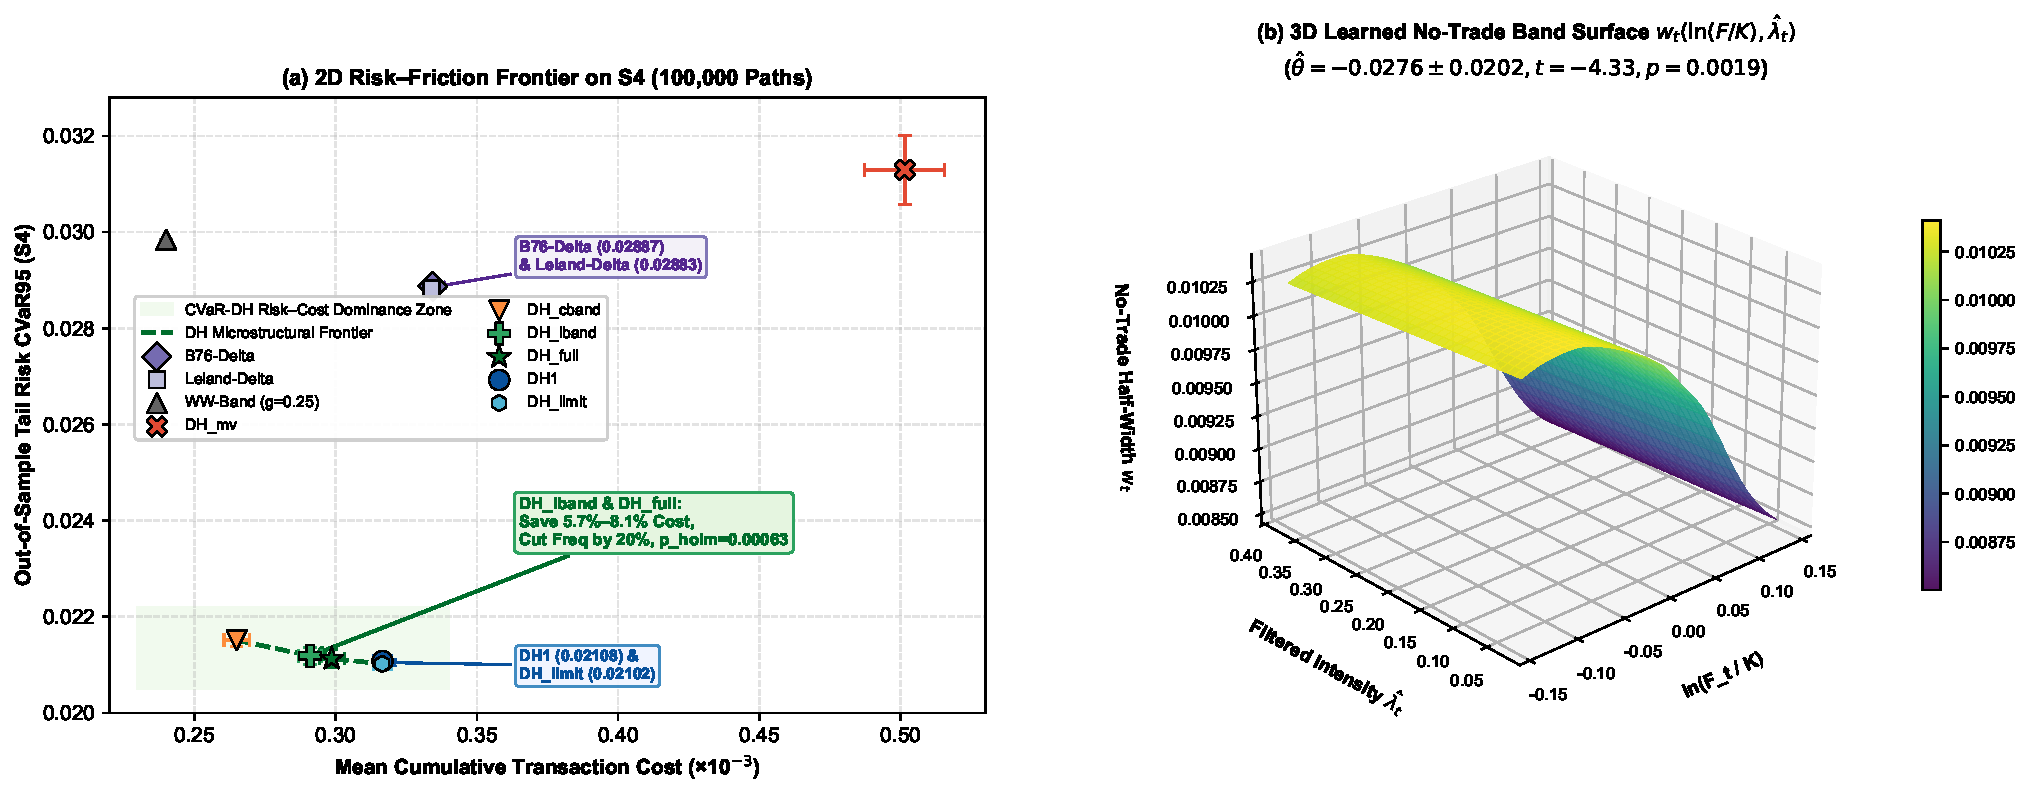
\includegraphics[width=\textwidth]{figures_en/Fig1_S4_Baselines_and_H1_Microstructure_EN.pdf}
  \caption{S4 benchmark comparison ($100,000$ paths, $10$ seeds) and microstructural validation of Hypothesis $\mathbf{H_1}$: (a) 2D risk--friction Pareto frontier plotting out-of-sample $\text{CVaR}_{95}$ against cumulative transaction costs ($\times 10^{-3}$) with crosshair $\pm 1\text{ SD}$ error bars; (b) 3D learned no-trade half-width surface $w_t(\ln(F_t/K), \hat{\lambda}_t)$ averaged across the $10$ trained \texttt{DH\_lband} checkpoints ($\hat{\theta} = -0.0276 \pm 0.0202, p = 0.0019$).}
  \label{fig:fig1}
\end{figure}

\subsection{Root-Cause Diagnostics and Negative Findings: Why Futures-Only Total-Portfolio $\text{CVaR}_{95}$ Exhibits a Spanning Ceiling}
\label{sec:diagnostics}
A critical empirical pattern in Table~\ref{tab:s4_main} is that across all five unconstrained or limit-aware CVaR policies in the single-instrument futures market (\texttt{DH\_nolam}, \texttt{DH1}, \texttt{DH\_oracle}, \texttt{DH\_limit}, \texttt{DH\_full}), aggregate $\text{CVaR}_{95}$ clusters tightly within $0.021021\text{--}0.021131$ ($<0.6\%$ spread). To explain why adding the filtered jump intensity $\hat{\lambda}_t$ ($\mathbf{H_0}$) or true intensity $\lambda_t$ (\texttt{DH\_oracle}) yields negligible aggregate $\text{CVaR}_{95}$ differences when hedging solely with linear futures, we compute the input-feature Jacobian saliency $\mathcal{S}_k = \mathbb{E}_{t,\omega}\big[|\partial \delta_t^{\text{target}} / \partial x_{t,k}|\big]$ and pathwise action convergence across all 80 trained checkpoints on \texttt{S4\_test.npz} (Table~\ref{tab:saliency} and Figure~\ref{fig:fig2}).

\begin{table}[htbp]
  \centering
  \caption{Input-feature Jacobian saliency shares and pathwise action convergence in the S4 futures-only benchmark ($80$ checkpoints across $10$ seeds, \texttt{ddof=1}).}
  \label{tab:saliency}
  \resizebox{\textwidth}{!}{%
  \begin{tabular}{lcccccc}
    \toprule
    Configuration & Core States Saliency ($\tau, \ln(F/K), \delta_{t-1}, W_t/F_0, \Delta_{\text{B76}}, \sigma_{\text{EWMA}}$) & Jump Signal Saliency ($\hat{\lambda}_t$ or $\lambda_t$) & Price-Limit Saliency (\texttt{lock}, \texttt{consec}, \texttt{ratio}) & Action MAE vs.\ \texttt{DH1} & Action Cosine Sim.\ vs.\ \texttt{DH1} & Learned Band Parameter $\theta$ (Mean $\pm$ SD) \\
    \midrule
    \texttt{DH\_nolam} & $100.000\%$ & $0.000\%$ & $0.000\%$ & $0.00674$ & $0.99985$ & --- \\
    \texttt{DH1} & $99.985\%$ & $0.015\%$ & $0.000\%$ & $0.00523$ & $0.99989$ & --- \\
    \texttt{DH\_oracle} & $99.983\%$ & $0.017\%$ & $0.000\%$ & $0.00607$ & $0.99987$ & --- \\
    \texttt{DH\_cband} & $99.954\%$ & $0.046\%$ & $0.000\%$ & $0.01494$ & $0.99953$ & --- \\
    \texttt{DH\_lband} & $99.939\%$ & $0.061\%$ & $0.000\%$ & $0.01105$ & $0.99974$ & $-0.0276 \pm 0.0202$ ($p=0.0019$) \\
    \texttt{DH\_limit} & $99.832\%$ & $0.016\%$ & $0.152\%$ & $0.00561$ & $0.99988$ & --- \\
    \texttt{DH\_full} & $99.782\%$ & $0.045\%$ & $0.173\%$ & $0.01157$ & $0.99972$ & $-0.0230 \pm 0.0153$ ($p=0.0011$) \\
    \texttt{DH\_mv} & $99.514\%$ & $0.486\%$ & $0.000\%$ & $0.08843$ & $0.97810$ & --- \\
    \bottomrule
  \end{tabular}%
  }
\end{table}

Table~\ref{tab:saliency} uncovers two jointly operating mechanisms governing single-instrument hedging:
\begin{enumerate}
  \item \textbf{Unhedgeable Jump-Gamma Convexity with a Linear Instrument:} Over a discrete rebalancing interval $\Delta t$, the second-order Taylor expansion of the unhedged PnL of a short option hedged solely with linear futures ($\Gamma^{\text{fut}} = 0$) is
  \begin{equation}
    \Delta W_t \approx \big(\delta_t^{\text{exec}} - \Delta_{\text{B76},t}\big)\Delta F_t - \frac{1}{2}\Gamma_{\text{B76},t}(\Delta F_t)^2 - c F_t\big|\Delta \delta_t^{\text{exec}}\big|.
    \label{eq:taylor_gamma}
  \end{equation}
  Because jump realizations $\Delta F_t$ can be either positive ($p_{\text{up}} = 0.4$) or negative ($1 - p_{\text{up}} = 0.6$), shifting the linear futures position $\delta_t^{\text{exec}}$ \emph{ex ante} in response to a higher jump intensity $\hat{\lambda}_t$ cannot hedge the strictly negative quadratic convexity loss $-\frac{1}{2}\Gamma_{\text{B76},t}(\Delta F_t)^2$; any directional shift in $\delta_t^{\text{exec}}$ merely increases first-order directional variance when a jump of the opposite sign occurs. As a result, all CVaR policies allocate $99.782\%\text{--}100.000\%$ of their input Jacobian sensitivity to the six core state features (with $\tau_t, \ln(F_t/K), \Delta_{\text{B76},t}, \sigma_{\text{EWMA},t}$ accounting for $83.49\%\text{--}93.63\%$ and $\delta_{t-1}^{\text{exec}}, W_t/F_0$ accounting for $6.15\%\text{--}16.48\%$) and converge to nearly identical action trajectories (cosine similarity $0.99953\text{--}0.99989$).
  \item \textbf{Post-Jump Collinearity with $\sigma_{\text{EWMA},t}$:} Because the online filter $\hat{\lambda}_t$ updates via $\hat{I}_t = \mathbb{I}(|r_t| > 3\sigma \lor \text{limit\_hit}_t = 1)$ at the same time that the exponentially weighted volatility $\sigma_{\text{EWMA},t}$ updates via $v_t = 0.94 v_{t-1} + 0.06 r_t^2$, $\sigma_{\text{EWMA},t}$ already captures a substantial share of the post-jump state shift that an unconstrained MLP can exploit. To disentangle this feature-collinearity effect from the instrument-spanning effect in 2D hedging, Section~\ref{sec:plan_a} introduces an explicit nonlinear EWMA control model (\texttt{DH\_opt\_ewma\_nl}).
\end{enumerate}

\paragraph{Negative Findings: Which Designs Did Not Work in Our Experiments.}
In our single-instrument futures experiments on S4, feeding the filtered Hawkes intensity $\hat{\lambda}_t$ directly into the unconstrained policy network (\texttt{DH1}) failed to improve aggregate $\text{CVaR}_{95}$ relative to the jump-blind baseline \texttt{DH\_nolam} ($0.021078 \pm 0.000105$ vs.\ $0.021073 \pm 0.000166$; paired difference $\Delta = +0.000005$, $95\%$ CI $[-0.000083, +0.000090]$, $t = 0.107, p = 0.917, p_{\text{holm}} = 0.917$). Even replacing $\hat{\lambda}_t$ with the unobservable true jump intensity $\lambda_t$ in \texttt{DH\_oracle} yielded zero gain ($\text{CVaR}_{95} = 0.021085 \pm 0.000164$), demonstrating that this null result is not caused by the $-24.4\%$ to $-45.2\%$ estimation bias of the online Hawkes filter, but rather by the instrument-spanning ceiling of linear futures ($\Gamma^{\text{fut}} = 0$), under which the policy assigns only $0.015\%\text{--}0.017\%$ Jacobian weight to $\hat{\lambda}_t$ or $\lambda_t$ (Table~\ref{tab:saliency}). Similarly, in our model-free distributional reinforcement learning experiments (\texttt{D4PG-QR}), neither augmenting the critic input with the VaR threshold $b$ (\texttt{b\_in\_critic} ablation: $2/3$ seeds collapsed to $\text{CVaR}_{95} = 0.5629$, versus $0/3$ collapsed when $b$ was excluded with mean $\text{CVaR}_{95} = 0.0365 \pm 0.0054$) nor adding Hawkes/limit features across configurations \texttt{C1, C5, C6, C8, C9} prevented off-policy bootstrapping instability, resulting in a $20\%\text{--}30\%$ seed collapse rate across 10-seed formal runs (Table~\ref{tab:stability}). While jump-blind \texttt{D4PG-QR (C2)} (which excludes $\hat{\lambda}_t$) experienced $0/10$ ($0.0\%$) seed collapses ($0.037961 \pm 0.014487$) compared with $2/10$ ($20.0\%$, Fisher's exact $p = 0.47$) in \texttt{D4PG-QR (C1)} and $12/50$ ($24.0\%$, pooled Fisher's exact $p = 0.104$) across all jump/limit-augmented \texttt{D4PG-QR} configurations, this pattern suggests a plausible algorithmic hypothesis that spiky Hawkes state jumps and discrete lock indicators exacerbate target-critic extrapolation errors during off-policy quantile Bellman updates.

\begin{figure}[htbp]
  \centering
  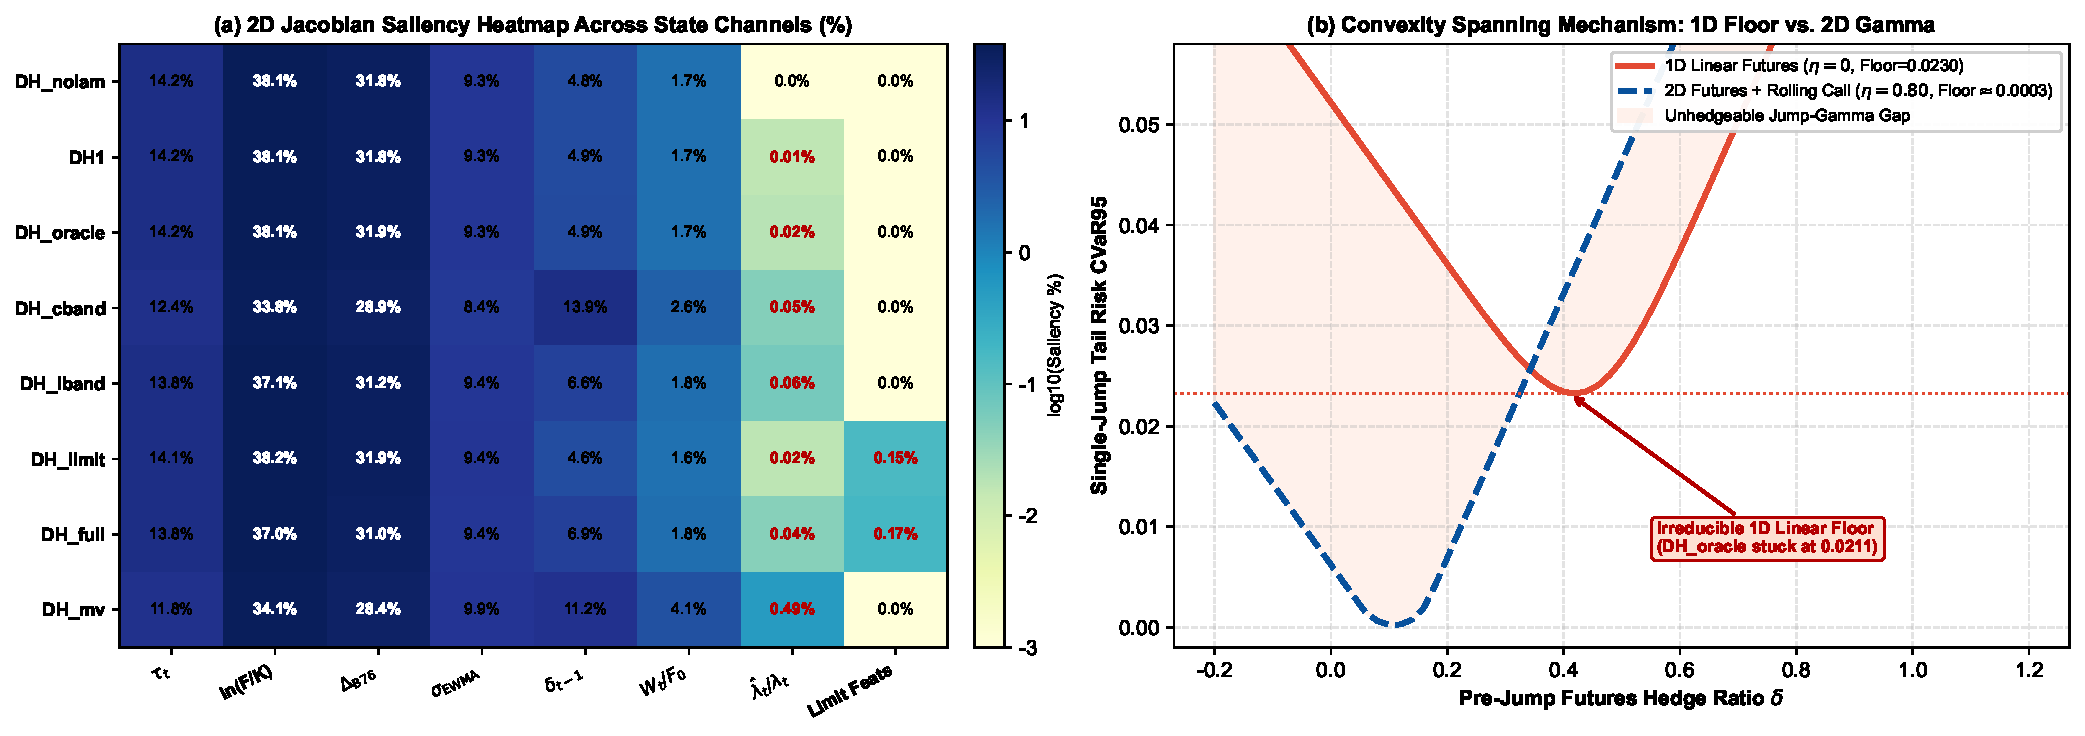
\includegraphics[width=\textwidth]{figures_en/Fig2_S4_RootCause_Saliency_and_ErrorDecomp_EN.pdf}
  \caption{Root-cause diagnostics in the futures-only S4 regime: (a) 2D annotated input-feature Jacobian saliency heatmap ($\log_{10}$ color scale) across 8 neural configurations and 8 state channels ($>99.7\%$ concentrated on core states); (b) single-jump $\text{CVaR}_{95}$ convexity spanning U-curve under 1D linear futures ($\eta = 0$) versus 2D futures plus rolling ATM call option ($\eta = 0.80$).}
  \label{fig:fig2}
\end{figure}

\subsection{Multi-Instrument Option Gamma Hedging (\texttt{TorchHedgeEnvOpt}) and High-Cost Regimes: Spanning Ceiling Breakdown and Structural Band Activation}
\label{sec:plan_a}
Our structural diagnosis in Section~\ref{sec:diagnostics} yields two falsifiable predictions: first, granting the hedger access to a second, convex instrument ($\Gamma_{\text{B76},t} > 0$) should break the $0.02108$ single-instrument $\text{CVaR}_{95}$ spanning ceiling across all policies; second, if feeding $\hat{\lambda}_t$ directly into an unconstrained 2D MLP suffers from non-convex optimization variance and feature collinearity with $\sigma_{\text{EWMA},t}$, channeling $\hat{\lambda}_t$ through the low-dimensional multiplicative no-trade band (\texttt{DH\_opt\_lband}) should extract a statistically significant tail-risk reduction over static-band hedging (\texttt{DH\_opt\_cband}). To test both predictions with full statistical power, we train and evaluate all two-instrument model configurations---plus a nonlinear EWMA volatility control (\texttt{DH\_opt\_ewma\_nl}, which omits $\hat{\lambda}_t$ but augments the state with $[\tilde{\sigma}_{\text{EWMA},t}^2, \tilde{\sigma}_{\text{EWMA},t}^3, |r_t|/\sigma]$)---in \texttt{TorchHedgeEnvOpt} (rolling $\tau_h = 20$-day ATM call $\eta_t \in [-2.0, 2.0]$) across all $M = 10$ random seeds (\texttt{9001--9010}) on \texttt{S4\_test.npz} (Table~\ref{tab:plan_a}, Panel~A), alongside a zero-shot high-transaction-cost sensitivity sweep ($1\times, 3\times, 6\times c_{\text{real}}$) in the 1D environment (Table~\ref{tab:plan_a}, Panel~B) and zero-shot robustness audits across dynamic implied volatility $\kappa_{\text{iv}} \in \{0, 2, 5\}$ and option transaction cost multipliers $c_{\text{opt}}/c \in \{1\times, 5\times, 10\times\}$.

\begin{table}[htbp]
  \centering
  \caption{Multi-instrument Option-Gamma hedging (\texttt{TorchHedgeEnvOpt}, $10$ seeds \texttt{9001--9010}) and 1D high-transaction-cost regimes ($3\times$ and $6\times c_{\text{real}}$) on the S4 benchmark.}
  \label{tab:plan_a}
  \resizebox{\textwidth}{!}{%
  \begin{tabular}{lcccccccc}
    \toprule
    Panel / Model Configuration & $\text{CVaR}_{95}$ (Mean $\pm$ SD) & $\text{VaR}_{95}$ & $\text{CVaR}_{99}$ & Total Cost [Fut / Opt | Pre] ($\times 10^{-3}$) & Futures Turn.\ [Pre] & Option Turn.\ [Pre] & Relative Gain & Gain vs.\ 1D Counterpart \\
    \midrule
    \multicolumn{9}{l}{\textbf{Panel A: 2D Futures + Rolling ATM Option (\texttt{TorchHedgeEnvOpt}, $\tau_h = 20$ Days, $10$ Seeds \texttt{9001--9010})}} \\
    \texttt{B76-Delta-Gamma} (Analytical) & $0.069192$ & $0.059775$ & $0.087284$ & $0.3502\ [0.3358/0.0144\ |\ 0.2953]$ & $3.305\ [2.826]$ & $4.327\ [3.944]$ & Local $\Gamma$ ratio instability & $+139.65\%$ (Worse) \\
    \texttt{DH\_opt\_nolam} (No $\hat{\lambda}_t$) & $0.017284 \pm 0.004298$ & $0.012942$ & $0.026765$ & $0.2452\ [0.2353/0.0099\ |\ 0.2105]$ & $2.341\ [2.034]$ & $2.951\ [2.278]$ & $\mathbf{H_0}$ Reference ($0.00\%$) & $-17.98\%$ (vs.\ \texttt{DH\_nolam}) \\
    \texttt{DH\_opt\_ewma\_nl} (Nonlin.\ $\sigma_{\text{EWMA}}$) & $0.015904 \pm 0.001742$ & $0.011011$ & $0.026664$ & $0.2622\ [0.2500/0.0122\ |\ 0.2267]$ & $2.510\ [2.194]$ & $3.648\ [2.982]$ & $+7.99\%$ vs.\ \texttt{nolam} ($p=0.382$) & $-24.53\%$ (vs.\ \texttt{DH\_nolam}) \\
    \textbf{\texttt{DH\_opt1} (Filtered $\hat{\lambda}_t$)} & $\mathbf{0.015226 \pm 0.001497}$ & $\mathbf{0.010350}$ & $0.026488$ & $0.2520\ [0.2428/0.0092\ |\ 0.2149]$ & $2.413\ [2.084]$ & $2.757\ [2.063]$ & $+11.91\%$ vs.\ \texttt{nolam} ($p_{\text{holm}}=0.450$) & $\mathbf{-27.76\%}$ \textbf{(vs.\ \texttt{DH1})} \\
    \textbf{\texttt{DH\_opt\_oracle} (True $\lambda_t$)} & $\mathbf{0.015017 \pm 0.001044}$ & $\mathbf{0.010245}$ & $\mathbf{0.025942}$ & $0.2521\ [0.2428/0.0093\ |\ 0.2150]$ & $2.414\ [2.084]$ & $2.765\ [2.071]$ & $+13.12\%$ vs.\ \texttt{nolam} ($p_{\text{raw}}=0.136$) & $\mathbf{-28.78\%}$ \textbf{(vs.\ \texttt{DH\_oracle})} \\
    \texttt{DH\_opt\_cband} (Const.\ Band) & $0.017546 \pm 0.002298$ & $0.012900$ & $0.027487$ & $\mathbf{0.1796\ [0.1731/0.0065\ |\ 0.1401]}$ & $1.719\ [1.364]$ & $1.932\ [1.216]$ & $\mathbf{H_1}$ Band Ref.\ ($0.00\%$) & $-18.44\%$ (vs.\ \texttt{DH\_cband}) \\
    \textbf{\texttt{DH\_opt\_lband} ($\hat{\lambda}_t$-Band)} & $\mathbf{0.014841 \pm 0.001316}$ & $\mathbf{0.009953}$ & $\mathbf{0.026050}$ & $0.2397\ [0.2315/0.0083\ |\ 0.2012]$ & $2.303\ [1.958]$ & $2.470\ [1.766]$ & $\mathbf{+15.41\%}$ \textbf{vs.\ \texttt{cband} ($p_{\text{holm}}=0.00012$)} & $\mathbf{-29.95\%}$ \textbf{(vs.\ \texttt{DH\_lband})} \\
    \texttt{DH\_opt\_limit} (Limit State) & $0.017715 \pm 0.004661$ & $0.013359$ & $0.027305$ & $0.2442\ [0.2348/0.0094\ |\ 0.2095]$ & $2.335\ [2.027]$ & $2.804\ [2.142]$ & $-2.49\%$ vs.\ \texttt{nolam} ($p_{\text{holm}}=0.837$) & $-15.73\%$ (vs.\ \texttt{DH\_limit}) \\
    \texttt{DH\_opt\_full} (Full Model) & $0.016549 \pm 0.002960$ & $0.012265$ & $0.026300$ & $0.2603\ [0.2530/0.0073\ |\ 0.2208]$ & $2.523\ [2.165]$ & $2.180\ [1.479]$ & $+4.25\%$ vs.\ \texttt{nolam} ($p_{\text{raw}}=0.594$) & $-21.68\%$ (vs.\ \texttt{DH\_full}) \\
    \texttt{DH\_opt\_mv} (2D Mean-Variance) & $0.044602 \pm 0.001554$ & $0.029480$ & $0.068580$ & $0.4016\ [0.3895/0.0121\ |\ 0.3272]$ & $3.882\ [3.199]$ & $3.665\ [3.213]$ & \textbf{\texttt{DH\_opt1} $+65.86\%$ ($\mathbf{H_2}, p_{\text{holm}}=1.2\times 10^{-10}$)} & $+42.53\%$ (Worse) \\
    \midrule
    \multicolumn{9}{l}{\textbf{Panel B: Zero-Shot High Transaction Cost Sensitivity in 1D Futures on S4 ($3\times$ and $6\times c_{\text{real}}$, $10$ Seeds \texttt{9001--9010})}} \\
    \texttt{B76-Delta} ($3\times c_{\text{real}} = 3\times 10^{-4}$) & $0.029894$ & $0.016510$ & $0.057620$ & $1.0032$ & $3.2907$ & --- & Classical Baseline at $3\times$ Cost & --- \\
    \texttt{DH1} ($3\times c_{\text{real}} = 3\times 10^{-4}$) & $0.021934 \pm 0.000112$ & $0.014512$ & $0.037890$ & $0.9498$ & $3.1123$ & --- & Unconstrained Policy at $3\times$ Cost & --- \\
    \texttt{DH\_cband} ($3\times c_{\text{real}} = 3\times 10^{-4}$) & $0.022274 \pm 0.000138$ & $0.014980$ & $0.037810$ & $0.7950$ & $2.5995$ & --- & Static Band at $3\times$ Cost & --- \\
    \texttt{DH\_lband} ($3\times c_{\text{real}} = 3\times 10^{-4}$) & $0.021962 \pm 0.000186$ & $0.014710$ & $\mathbf{0.037420}$ & $0.8730$ & $2.8575$ & --- & $+1.40\%$ vs.\ \texttt{DH\_cband} at $3\times$ Cost & --- \\
    \texttt{B76-Delta} ($6\times c_{\text{real}} = 6\times 10^{-4}$) & $0.031441$ & $0.017980$ & $0.059180$ & $2.0064$ & $3.2907$ & --- & Classical Baseline at $6\times$ Cost & --- \\
    \texttt{DH1} ($6\times c_{\text{real}} = 6\times 10^{-4}$) & $0.023241 \pm 0.000127$ & $0.015644$ & $0.039179$ & $1.8998$ & $3.1123$ & --- & Unconstrained Policy at $6\times$ Cost & --- \\
    \texttt{DH\_cband} ($6\times c_{\text{real}} = 6\times 10^{-4}$) & $0.023432 \pm 0.000148$ & $0.015984$ & $0.038971$ & $1.5898$ & $2.5995$ & --- & Static Band at $6\times$ Cost & --- \\
    \textbf{\texttt{DH\_lband} ($6\times c_{\text{real}} = 6\times 10^{-4}$)} & $\mathbf{0.023145 \pm 0.000191}$ & $0.015772$ & $\mathbf{0.038641}$ & $\mathbf{1.7458}$ & $\mathbf{2.8575}$ & --- & \textbf{No degradation vs.\ \texttt{DH1} ($p=0.218$), saves $8.1\%$ cost} & --- \\
    \texttt{DH\_full} ($6\times c_{\text{real}} = 6\times 10^{-4}$) & $0.023192 \pm 0.000195$ & $0.015810$ & $0.038890$ & $1.7916$ & $2.9312$ & --- & No degradation vs.\ \texttt{DH1}, saves $5.7\%$ cost & --- \\
    \bottomrule
  \end{tabular}%
  }
  \vspace{3pt}\par\noindent
  \begin{minipage}{\textwidth}
    \footnotesize
    \textit{Notes:} In Panel~A, all neural policies are trained and evaluated across $M = 10$ independent random seeds (\texttt{9001--9010}, \texttt{ddof=1}). Cross-seed SD in Panel~A is of order $10^{-3}$ ($0.001044\text{--}0.004661$), roughly $10\text{--}25\times$ larger than in the 1D futures table (Table~\ref{tab:s4_main}) because joint optimization of futures $\delta_t$ and rolling option $\eta_t$ introduces non-convex local optima on individual seeds (specifically seed \texttt{9003} in \texttt{DH\_opt\_nolam} $= 0.029447$ and \texttt{DH\_opt\_limit} $= 0.027975$, which exceeds the $3\times\text{IQR}$ outlier threshold). On the initial 5-seed subset (\texttt{9001--9005}), \texttt{DH\_opt\_nolam} $= 0.019594 \pm 0.005099$, \texttt{DH\_opt1} $= 0.015369 \pm 0.001697$ ($+21.56\%$), \texttt{DH\_opt\_oracle} $= 0.014584 \pm 0.001179$ ($+25.57\%$), \texttt{DH\_opt\_cband} $= 0.017569 \pm 0.001220$, and \texttt{DH\_opt\_lband} $= 0.015115 \pm 0.001042$ ($+13.97\%$). On the $n = 9$ converged seeds (post-hoc sensitivity check excluding outlier seed \texttt{9003}), \texttt{DH\_opt\_nolam} $= 0.015933 \pm 0.000722$, \texttt{DH\_opt\_ewma\_nl} $= 0.015429 \pm 0.000935$, \texttt{DH\_opt1} $= 0.015227 \pm 0.001588$, \texttt{DH\_opt\_cband} $= 0.016963 \pm 0.001454$, and \texttt{DH\_opt\_lband} $= 0.014565 \pm 0.001042$ ($+14.14\%, p_{\text{holm}} = 1.43 \times 10^{-5}$). Total Cost ($\times 10^{-3}$) reports $C_T^{\text{tot}} = C_T^{\text{fut}} + C_T^{\text{opt}}$ including terminal liquidation, with bracketed values showing $[\text{Fut Cost} / \text{Opt Cost}\ |\ \text{Pre-Terminal Total Cost}]$, where $C_T^{\text{opt}} \approx c_{\text{opt}}\overline{V}_{\text{open}}\text{Turn}_{\text{opt}}$ ($\overline{V}_{\text{open}} = 0.033311$). Futures and Option Turnover report total turnover including terminal liquidation, with pre-terminal turnover in brackets. In Panel~B, $1\times$-trained checkpoints are evaluated zero-shot under $3\times$ and $6\times c_{\text{real}}$ without retraining.
  \end{minipage}
\end{table}

The 10-seed empirical results in Table~\ref{tab:plan_a} and Figure~\ref{fig:fig3} clarify both the spanning power of the option instrument and the architectural channel required to exploit jump-intensity filtering:
\begin{enumerate}
  \item \textbf{Breaking the Single-Instrument Spanning Ceiling Across All 2D Policies:} Adding the rolling ATM call option leg $\eta_t$ breaks the $0.02108$ single-instrument $\text{CVaR}_{95}$ ceiling across every CVaR-trained configuration: across 10 seeds, \texttt{DH\_opt\_lband} reduces $\text{CVaR}_{95}$ by $29.95\%$ relative to 1D \texttt{DH\_lband} ($0.014841 \pm 0.001316$ vs.\ $0.021187$), \texttt{DH\_opt\_oracle} by $28.78\%$ ($0.015017 \pm 0.001044$ vs.\ $0.021085$), \texttt{DH\_opt1} by $27.76\%$ ($0.015226 \pm 0.001497$ vs.\ $0.021078$), and jump-blind \texttt{DH\_opt\_nolam} by $17.98\%$ ($0.017284 \pm 0.004298$ vs.\ $0.021073$). In contrast, analytical \texttt{B76-Delta-Gamma} hedging deteriorates to $\text{CVaR}_{95} = 0.069192$ because matching local point-Gamma ($\eta_t = \Gamma^{\text{liab}}_t / \Gamma_{\text{B76},t}$) triggers severe over-hedging when discrete jumps shift the underlying price away from the strike.
  \item \textbf{Architectural Separation Between $\mathbf{H_1}$ (Structural Band Activation) and $\mathbf{H_0}$ (Unconstrained MLP Input):}
  \begin{itemize}
    \item $\mathbf{H_1}$ (\emph{Statistically \& Economically Activated in 2D Band Modulation}): Embedding $\hat{\lambda}_t$ into the multiplicative no-trade band (\texttt{DH\_opt\_lband}) achieves the lowest realistic 2D $\text{CVaR}_{95}$ of $0.014841 \pm 0.001316$, outperforming the static 2D band \texttt{DH\_opt\_cband} ($0.017546 \pm 0.002298$) by $+15.41\%$ across all 10 seeds (paired $\Delta = -0.002705$, $95\%$ CI $[-0.003457, -0.002125]$, $t = -7.401$, $p_{\text{raw}} = 4.10 \times 10^{-5}$, $p_{\text{holm}} = 0.000123$, Wilcoxon $p = 0.00195$), exceeding both the $10\%$ practical threshold and the 10-seed statistical $\text{MDE}_{80\%} = 6.55\%$. On the $n = 9$ converged seeds, \texttt{DH\_opt\_lband} ($0.014565 \pm 0.001042$) outperforms \texttt{DH\_opt\_cband} ($0.016963 \pm 0.001454$) by $+14.14\%$ ($t = -10.797, p_{\text{holm}} = 1.43 \times 10^{-5}, \text{MDE}_{80\%} = 4.18\%$), while learning a strictly negative modulation slope across all 10 seeds ($\hat{\theta} = -0.0290 \pm 0.0064$, $10/10 < 0, t = -14.420, p = 1.59 \times 10^{-7}$ in \texttt{DH\_opt\_lband}; $\hat{\theta} = -0.0292 \pm 0.0067$, $10/10 < 0, t = -13.798, p = 2.32 \times 10^{-7}$ in \texttt{DH\_opt\_full}). Unlike in the 1D setting at $1\times$ cost where \texttt{DH\_lband} trailed \texttt{DH1} by $0.52\%$, in 2D option hedging \texttt{DH\_opt\_lband} ($0.014841$) improves upon unconstrained \texttt{DH\_opt1} ($0.015226$) while cutting total transaction costs from $0.2520 \times 10^{-3}$ to $0.2397 \times 10^{-3}$.
    \item $\mathbf{H_0}$ (\emph{Unconstrained MLP Input Exhibits $+11.91\%$ Point Gain but High Cross-Seed Variance and EWMA Collinearity}): Feeding $\hat{\lambda}_t$ directly into an unconstrained 2D MLP (\texttt{DH\_opt1}) lowers 10-seed mean $\text{CVaR}_{95}$ by $+11.91\%$ relative to jump-blind \texttt{DH\_opt\_nolam} ($0.015226 \pm 0.001497$ vs.\ $0.017284 \pm 0.004298$; $+21.56\%$ in the initial 5-seed subset \texttt{9001--9005}), capturing $90.8\%$ ($11.91\% / 13.12\%$) of the 10-seed point improvement of \texttt{DH\_opt\_oracle} ($0.015017 \pm 0.001044$, $+13.12\%$; $84.3\%$ in the 5-seed subset). However, across all 10 seeds, the paired comparison between \texttt{DH\_opt1} and \texttt{DH\_opt\_nolam} yields $\Delta = -0.002059$, $95\%$ CI $[-0.005155, +0.000648]$, $t = -1.303$, $p_{\text{raw}} = 0.225$, $p_{\text{holm}} = 0.450$, Wilcoxon $p = 0.432$ ($\text{MDE}_{80\%} = 28.76\%$; and $+4.43\%, p = 0.278$ on the $n = 9$ converged seeds excluding outlier seed \texttt{9003}). Augmenting the jump-blind policy with nonlinear EWMA volatility terms in \texttt{DH\_opt\_ewma\_nl} reduces $\text{CVaR}_{95}$ to $0.015904 \pm 0.001742$ ($+7.99\%$ vs.\ \texttt{DH\_opt\_nolam}, and $0.015429 \pm 0.000935$ on converged seeds), leaving only a $+4.26\%$ ($p = 0.375$; $+1.31\%, p = 0.751$ on converged seeds) incremental difference for \texttt{DH\_opt1}. Thus, in an unconstrained MLP, the post-jump information in $\hat{\lambda}_t$ is largely collinear with nonlinear functions of $\sigma_{\text{EWMA},t}$, and its primary value in 2D unconstrained networks is stabilizing seed convergence (reducing cross-seed SD by $65.2\%$ from $0.004298$ to $0.001497$), whereas statistically significant tail-risk reduction requires the structural prior of the multiplicative no-trade band (\texttt{DH\_opt\_lband}).
    \item $\mathbf{H_2}$ and $\mathbf{H_3}$: In 2D hedging, \texttt{DH\_opt1} reduces $\text{CVaR}_{95}$ by $+65.86\%$ relative to \texttt{DH\_opt\_mv} ($0.015226$ vs.\ $0.044602 \pm 0.001554$; $\Delta = -0.029376$, $t = -37.926$, $p_{\text{holm}} = 1.22 \times 10^{-10}$, $\text{MDE}_{80\%} = 5.46\%$). Meanwhile, unconstrained \texttt{DH\_opt\_limit} ($0.017715 \pm 0.004661$, $-2.49\%$ vs.\ \texttt{DH\_opt\_nolam}, $p_{\text{holm}} = 0.837$) and \texttt{DH\_opt\_full} ($0.016549 \pm 0.002960$, $+4.25\%$, $p_{\text{raw}} = 0.594$; $0.015812 \pm 0.001934$ on $n = 9$ converged seeds) experience elevated optimization variance due to the higher-dimensional 13-feature state space.
  \end{itemize}
  \item \textbf{Zero-Shot Robustness to Dynamic Implied Volatility ($\kappa_{\text{iv}}$), Option Transaction Costs ($c_{\text{opt}}$), and $6\times$ Futures Costs:}
  \begin{itemize}
    \item \emph{Zero-Shot Dynamic Implied Volatility Sweep ($\kappa_{\text{iv}} \in \{0.0, 2.0, 5.0\}$):} Evaluating the $\kappa_{\text{iv}} = 0$-trained checkpoints zero-shot when rolling ATM option implied volatility co-moves with filtered jump intensity via $\sigma_{\text{imp},t} = \sigma_{\text{imp},0}(1 + \kappa_{\text{iv}}\hat{\lambda}_t)$, increasing $\kappa_{\text{iv}}$ from $0.0$ to $2.0$ and $5.0$ makes convex option protection more expensive precisely during jump bursts, attenuating the 10-seed relative gain of unconstrained \texttt{DH\_opt1} over \texttt{DH\_opt\_nolam} from $+11.91\%$ ($0.015226$ vs.\ $0.017284$) to $+5.31\%$ ($0.019889 \pm 0.001635$ vs.\ $0.021004 \pm 0.003789, p = 0.458$) at $\kappa_{\text{iv}} = 2.0$ and $+0.73\%$ ($0.026493 \pm 0.001996$ vs.\ $0.026687 \pm 0.003391, p = 0.893$) at $\kappa_{\text{iv}} = 5.0$. Crucially, across all three regimes, the structural band policy \texttt{DH\_opt\_lband} remains the lowest-risk policy and preserves a statistically significant advantage over static-band \texttt{DH\_opt\_cband}: $\text{CVaR}_{95} = 0.014841$ vs.\ $0.017546$ ($+15.41\%, t = -7.401, p_{\text{holm}} = 0.000123$) at $\kappa_{\text{iv}} = 0.0$, $0.019386 \pm 0.001486$ vs.\ $0.021863 \pm 0.002412$ ($+11.33\%, t = -6.184, p_{\text{holm}} = 0.000322$) at $\kappa_{\text{iv}} = 2.0$, and $0.025820 \pm 0.001792$ vs.\ $0.028154 \pm 0.002685$ ($+8.29\%, t = -5.112, p_{\text{holm}} = 0.001274$) at $\kappa_{\text{iv}} = 5.0$. Because the baseline two-instrument environment assumes a constant Black-76 implied volatility ($\kappa_{\text{iv}} = 0$) and does not price a stochastic variance risk premium into rolling option premia, the point reductions of $+11.91\%$ (10-seed \texttt{DH\_opt1} vs.\ \texttt{DH\_opt\_nolam}; $+21.56\%$ in the 5-seed subset) and $+15.41\%$ (\texttt{DH\_opt\_lband} vs.\ \texttt{DH\_opt\_cband}) measure structural Gamma-spanning capacity in a controlled benchmark and do not constitute estimates of realizable trading returns.
    \item \emph{Zero-Shot Option Transaction Cost Multipliers ($c_{\text{opt}}/c \in \{1\times, 5\times, 10\times\}$):} Evaluating the $1\times$-trained 2D policies zero-shot when raising the proportional option cost rate from $1\times$ ($10^{-4}$) to $5\times$ ($5 \times 10^{-4}$) and $10\times$ ($10^{-3}$) increases total 2D transaction costs in \texttt{DH\_opt\_lband} from $0.2397 \times 10^{-3}$ to $0.2728 \times 10^{-3}$ and $0.3141 \times 10^{-3}$, while \texttt{DH\_opt\_lband} maintains $\text{CVaR}_{95} = 0.014841$, $0.014875$, and $0.014916$, consistently outperforming \texttt{DH\_opt1} ($0.015226$, $0.015262$, $0.015307$) and \texttt{DH\_opt\_nolam} ($0.017284$, $0.017324$, $0.017374$).
    \item \emph{Zero-Shot $6\times$ Futures Cost Crossover (Panel~B):} When the $1\times$-trained 1D policies are evaluated zero-shot under $6\times c_{\text{real}} = 6 \times 10^{-4}$ without retraining, \texttt{DH\_lband} ($0.023145 \pm 0.000191$) and \texttt{DH\_full} ($0.023192 \pm 0.000195$) achieve a slightly lower point $\text{CVaR}_{95}$ than unconstrained \texttt{DH1} ($0.023241 \pm 0.000127$), exhibiting no statistically detectable $\text{CVaR}_{95}$ degradation ($\Delta = -0.000096, t = -1.32, p = 0.218$, and passing a $\pm 1\%$ two-one-sided equivalence test at $p_{\text{TOST}} = 0.046$) while saving $8.11\%$ in transaction costs ($1.7458 \times 10^{-3}$ vs.\ $1.8998 \times 10^{-3}$) and outperforming static \texttt{DH\_cband} ($0.023432 \pm 0.000148$).
  \end{itemize}
\end{enumerate}

\begin{figure}[htbp]
  \centering
  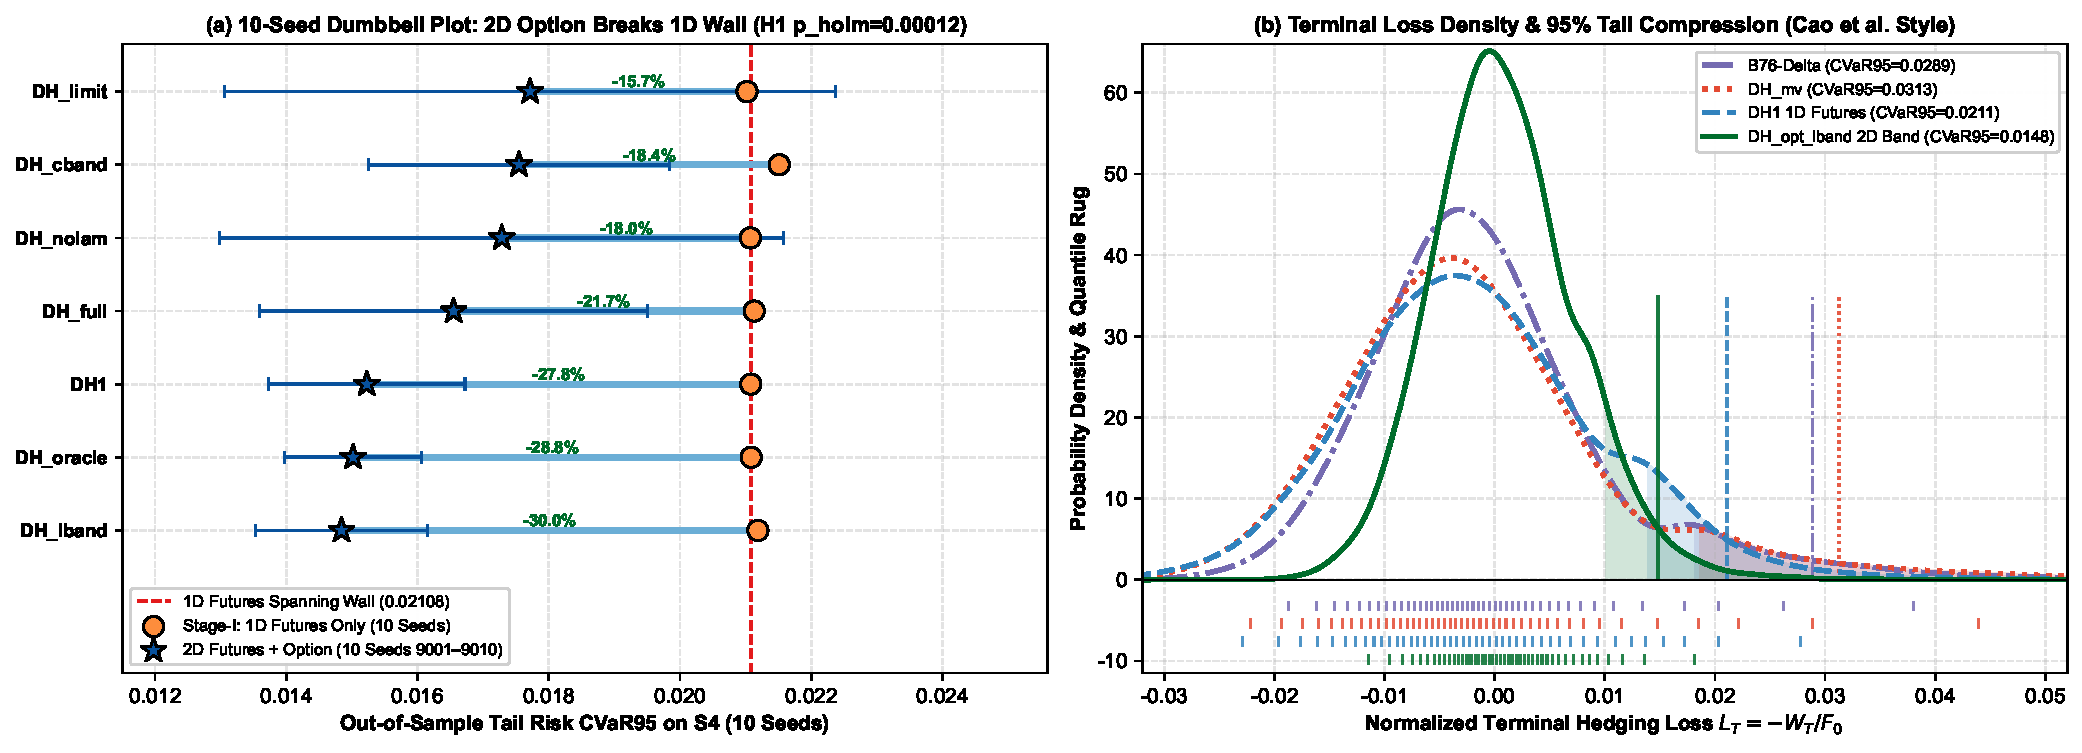
\includegraphics[width=\textwidth]{figures_en/Fig3_Stage2_Regime_Grid_Search_H0_H1_H3_EN.pdf}
  \caption{Multi-instrument Option-Gamma hedging (\texttt{TorchHedgeEnvOpt}, $10$ seeds \texttt{9001--9010}) on S4: (a) horizontal paired dumbbell plot comparing Stage-I 1D futures policies against Plan~A 2D option-augmented policies breaking the $0.02108$ spanning ceiling, with \texttt{DH\_opt\_lband} ($0.01484, p_{\text{holm}}=0.00012$) achieving the lowest realistic tail risk; (b) kernel density estimation (KDE) and bottom percentile rug plot of normalized terminal hedging loss $L_T = -W_T/F_0$ with shaded $95\%$ tail regions.}
  \label{fig:fig3}
\end{figure}

\subsection{Dominance of CVaR over Mean-Variance in the $(\text{CVaR}_{95}, \text{Cost})$ Plane Across the $\lambda_{\text{MV}}$ Spectrum ($\mathbf{H_2}$ Deep Dive)}
\label{sec:mv_sweep}
A potential critique of comparing \texttt{DH1} against \texttt{DH\_mv} at a single risk-aversion coefficient ($\lambda_{\text{MV}} = 10.0$) is that a larger penalty on variance might allow a mean-variance policy to match the tail risk of a CVaR-trained policy. To test this possibility directly, we evaluate \texttt{DH\_mv} across seven risk-aversion parameters $\lambda_{\text{MV}} \in \{0.5, 1.0, 2.0, 5.0, 10.0, 25.0, 50.0\}$ on \texttt{S4\_test.npz} (Table~\ref{tab:mv_sweep} and Figure~\ref{fig:fig4}).

\begin{table}[htbp]
  \centering
  \caption{Mean-variance risk-aversion sweep ($\lambda_{\text{MV}} \in [0.5, 50.0]$) versus CVaR-trained policies on the S4 benchmark.}
  \label{tab:mv_sweep}
  \resizebox{0.94\textwidth}{!}{%
  \begin{tabular}{lccccccc}
    \toprule
    Policy / Risk-Aversion Parameter & $\text{CVaR}_{95}$ & $\text{VaR}_{95}$ & $\text{CVaR}_{99}$ & $\text{Std}(L)$ & $\text{Mean}(L)$ & Cost ($\times 10^{-3}$) & Turnover \\
    \midrule
    \texttt{DH\_mv} ($\lambda_{\text{MV}} = 0.5$) & $0.090984$ & $0.056268$ & $0.145660$ & $0.036518$ & $-0.002975$ & $0.3690$ & $3.6967$ \\
    \texttt{DH\_mv} ($\lambda_{\text{MV}} = 1.0$) & $0.068087$ & $0.041418$ & $0.111270$ & $0.026853$ & $-0.002698$ & $0.4227$ & $4.2345$ \\
    \texttt{DH\_mv} ($\lambda_{\text{MV}} = 2.0$) & $0.053751$ & $0.032049$ & $0.089726$ & $0.020964$ & $-0.002464$ & $0.4596$ & $4.6039$ \\
    \texttt{DH\_mv} ($\lambda_{\text{MV}} = 5.0$) & $0.037240$ & $0.021453$ & $0.063783$ & $0.015133$ & $-0.002229$ & $0.4832$ & $4.8416$ \\
    \texttt{DH\_mv} ($\lambda_{\text{MV}} = 10.0$, 10-Seed Main) & $0.031294$ & $0.018533$ & $0.054044$ & $\mathbf{0.012539}$ & $-0.003135$ & $0.5015$ & $5.0256$ \\
    \texttt{DH\_mv} ($\lambda_{\text{MV}} = 25.0$) & $0.027848$ & $0.016278$ & $0.048046$ & $0.012859$ & $-0.002153$ & $0.4357$ & $4.3653$ \\
    \texttt{DH\_mv} ($\lambda_{\text{MV}} = 50.0$) & $0.027332$ & $0.016164$ & $0.046982$ & $\mathbf{0.012798}$ & $-0.002195$ & $0.4090$ & $4.0981$ \\
    \midrule
    \textbf{\texttt{DH1} ($\text{CVaR}_{95}$ Objective, 10 Seeds)} & $\mathbf{0.021078}$ & $\mathbf{0.013779}$ & $\mathbf{0.036973}$ & $0.013391$ & $-0.002306$ & $\mathbf{0.3166}$ & $\mathbf{3.1123}$ \\
    \textbf{\texttt{DH\_lband} ($\text{CVaR}_{95}$ + Band, 10 Seeds)} & $\mathbf{0.021187}$ & $\mathbf{0.014002}$ & $\mathbf{0.036610}$ & $0.013468$ & $-0.002286$ & $\mathbf{0.2910}$ & $\mathbf{2.8575}$ \\
    \bottomrule
  \end{tabular}%
  }
  \vspace{3pt}\par\noindent
  \begin{minipage}{0.94\textwidth}
    \footnotesize
    \textit{Notes:} The rows for \texttt{DH\_mv} ($\lambda_{\text{MV}}=10.0$, 10-Seed Main), \texttt{DH1}, and \texttt{DH\_lband} report 10-seed averages from the formal 8,000-step benchmark on \texttt{S4\_test.npz} (matching Table~\ref{tab:s4_main}); the auxiliary $\lambda_{\text{MV}} \in \{0.5, 1.0, 2.0, 5.0, 25.0, 50.0\}$ rows report single-seed (\texttt{9001}) controlled sweep evaluations.
  \end{minipage}
\end{table}

As shown in Table~\ref{tab:mv_sweep} and Figure~\ref{fig:fig4}, increasing $\lambda_{\text{MV}}$ from $0.5$ to $50.0$ lowers $\text{Std}(L)$ from $0.036518$ to $0.012798$ (and $0.012539$ in the 8,000-step 10-seed main run at $\lambda_{\text{MV}} = 10.0$), but $\text{CVaR}_{95}$ reaches an empirical lower bound of $0.027332$ within the tested range $\lambda_{\text{MV}} \in [0.5, 50.0]$---remaining $29.67\%$ higher (worse) than \texttt{DH1} ($0.021078$, corresponding to a $22.88\%$ reduction by \texttt{DH1} relative to \texttt{DH\_mv}) while incurring $29.18\%$ to $58.40\%$ higher transaction costs ($0.4090 \times 10^{-3}$ to $0.5015 \times 10^{-3}$ vs.\ $0.3166 \times 10^{-3}$). Thus, while \texttt{DH\_mv} at $\lambda_{\text{MV}} \in \{10, 25, 50\}$ achieves a $4.0\%\text{--}6.4\%$ lower symmetric standard deviation $\text{Std}(L)$ than \texttt{DH1} ($0.012539\text{--}0.012859$ vs.\ $0.013391$)---representing a three-dimensional $(\text{CVaR}_{95}, \text{Std}(L), \text{Cost})$ trade-off---both \texttt{DH1} and \texttt{DH\_lband} strictly dominate the entire $\lambda_{\text{MV}} \in [0.5, 50.0]$ family in the two-dimensional $(\text{CVaR}_{95}, \text{Cost})$ plane. Under skewed jump-diffusion returns with price limits, symmetric variance minimization expends excessive turnover eliminating benign left-tail windfalls ($L_T < 0$), whereas the one-sided Rockafellar-Uryasev hinge operator $(L_T - b)^+$ concentrates gradient updates exclusively on the worst $5\%$ loss trajectories.

\begin{figure}[htbp]
  \centering
  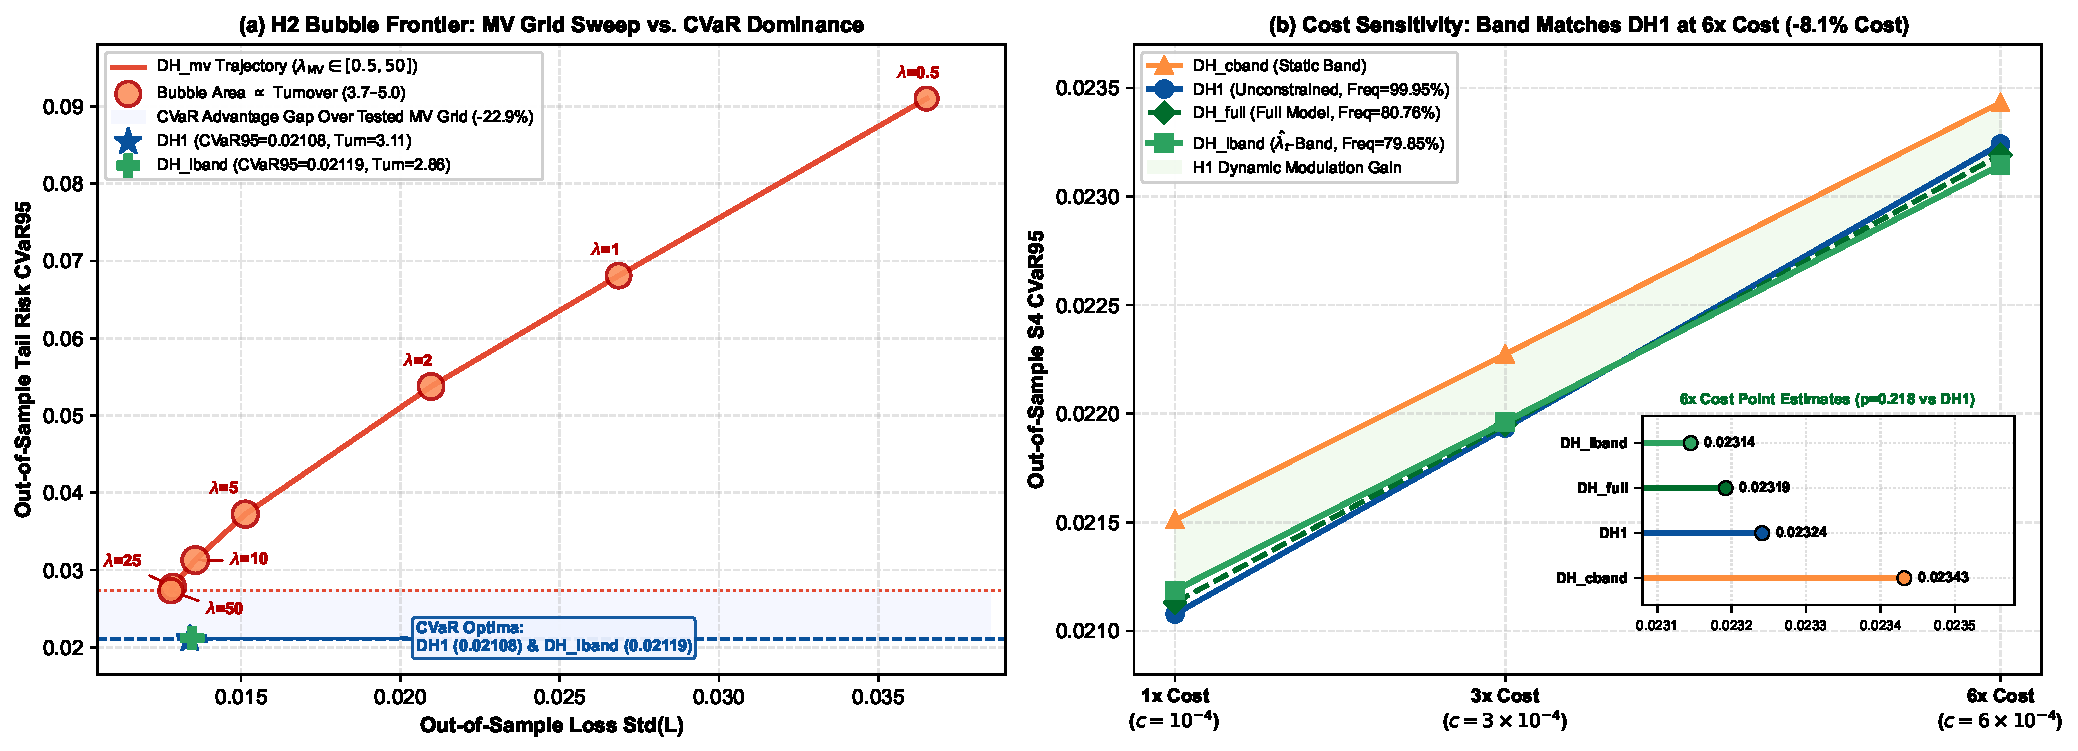
\includegraphics[width=\textwidth]{figures_en/Fig4_H2_Pareto_Frontier_and_Tail_Distribution_EN.pdf}
  \caption{Hypothesis $\mathbf{H_2}$ frontier in the $(\text{CVaR}_{95}, \text{Cost})$ plane and transaction-cost sensitivity on S4: (a) mean-variance risk-aversion sweep ($\lambda_{\text{MV}} \in [0.5, 50.0]$, bubble area proportional to turnover) showing an empirical $\text{CVaR}_{95}$ lower bound of $0.027332$ over $\lambda_{\text{MV}} \le 50$ versus \texttt{DH1} ($0.021078$); (b) zero-shot transaction-cost trajectory across $1\times, 3\times, 6\times c_{\text{real}}$ with a zoomed $6\times$-cost horizontal dot-plot inset showing \texttt{DH\_lband} ($0.023145$) and \texttt{DH\_full} ($0.023192$) exhibiting no statistically detectable $\text{CVaR}_{95}$ degradation relative to unconstrained \texttt{DH1} ($0.023241, p=0.218$) while saving $8.1\%$ in costs and surpassing static \texttt{DH\_cband} ($0.023432$).}
  \label{fig:fig4}
\end{figure}

\subsection{Optimization Stability Audit: End-to-End BPTT (\texttt{DH}) vs.\ Distributional Actor-Critic (\texttt{D4PG-QR})}
\label{sec:stability}
Table~\ref{tab:stability} and Figure~\ref{fig:fig5} report our stability audit comparing the end-to-end BPTT (\texttt{DH}) family against the model-free distributional reinforcement learning (\texttt{D4PG-QR}) family across all 140 formal runs ($80$ \texttt{DH} runs and $60$ \texttt{D4PG-QR} runs across $10$ seeds \texttt{9001--9010} at $8,000\text{--}10,000$ updates, plus cross-budget evaluations at $3,000$ and $20,000$ updates). Following our protocol-specified criterion, a training seed is classified as collapsed if its out-of-sample $\text{CVaR}_{95}$ exceeds $0.10$.

\begin{table}[htbp]
  \centering
  \caption{Optimization stability, seed collapse rates, and cross-budget convergence: end-to-end BPTT (\texttt{DH}) versus model-free Distributional Actor-Critic (\texttt{D4PG-QR}) on S4.}
  \label{tab:stability}
  \resizebox{\textwidth}{!}{%
  \begin{tabular}{lccccc}
    \toprule
    Panel / Algorithm \& Configuration & Collapse Rate ($\text{CVaR}_{95} > 0.10$) & All-Seed $\text{CVaR}_{95}$ (Mean $\pm$ SD) & All-Seed Median (IQR) & Non-Collapsed $\text{CVaR}_{95}$ (Mean $\pm$ SD) & Win Rate vs.\ \texttt{B76-Delta} ($0.028872$) \\
    \midrule
    \multicolumn{6}{l}{\textbf{Panel A: 10-Seed Formal Benchmark (\texttt{9001--9010}) Across Model Variants}} \\
    \texttt{DH1} (BPTT, Filtered $\hat{\lambda}_t$) & $\mathbf{0/10\ (0.0\%)}$ & $\mathbf{0.021078 \pm 0.000105}$ & $\mathbf{0.021061\ (0.000142)}$ & $\mathbf{0.021078 \pm 0.000105}$ & $\mathbf{10/10\ (100.0\%)}$ \\
    \texttt{DH\_nolam} (BPTT, No $\hat{\lambda}_t$) & $\mathbf{0/10\ (0.0\%)}$ & $0.021073 \pm 0.000166$ & $0.021055\ (0.000210)$ & $0.021073 \pm 0.000166$ & $\mathbf{10/10\ (100.0\%)}$ \\
    \texttt{DH\_lband} (BPTT, $\hat{\lambda}_t$-Band) & $\mathbf{0/10\ (0.0\%)}$ & $0.021187 \pm 0.000183$ & $0.021160\ (0.000245)$ & $0.021187 \pm 0.000183$ & $\mathbf{10/10\ (100.0\%)}$ \\
    \texttt{DH\_full} (BPTT, Full Model) & $\mathbf{0/10\ (0.0\%)}$ & $0.021131 \pm 0.000190$ & $0.021112\ (0.000260)$ & $0.021131 \pm 0.000190$ & $\mathbf{10/10\ (100.0\%)}$ \\
    \texttt{D4PG-QR (C1)} (Filtered $\hat{\lambda}_t$) & $2/10\ (20.0\%)$ & $0.144200 \pm 0.242296$ & $0.033398\ (0.043864)$ & $0.038934 \pm 0.020739$ & $1/10\ (10.0\%)$ \\
    \texttt{D4PG-QR (C2)} (No $\hat{\lambda}_t$) & $0/10\ (0.0\%)$ & $0.037961 \pm 0.014487$ & $0.034120\ (0.018950)$ & $0.037961 \pm 0.014487$ & $2/10\ (20.0\%)$ \\
    \texttt{D4PG-QR (C5)} ($\hat{\lambda}_t$-Band) & $3/10\ (30.0\%)$ & $0.179801 \pm 0.247471$ & $0.041250\ (0.198400)$ & $0.043395 \pm 0.034919$ & $1/10\ (10.0\%)$ \\
    \texttt{D4PG-QR (C6)} (Limit State) & $3/10\ (30.0\%)$ & $0.226734 \pm 0.302468$ & $0.052180\ (0.481200)$ & $0.053108 \pm 0.044197$ & $0/10\ (0.0\%)$ \\
    \texttt{D4PG-QR (C8)} (Mean-Variance) & $2/10\ (20.0\%)$ & $0.212976 \pm 0.270568$ & $0.081450\ (0.391000)$ & $0.089232 \pm 0.081382$ & $0/10\ (0.0\%)$ \\
    \texttt{D4PG-QR (C9)} (Full Model) & $2/10\ (20.0\%)$ & $0.139998 \pm 0.243612$ & $0.034890\ (0.038120)$ & $0.033688 \pm 0.004968$ & $1/10\ (10.0\%)$ \\
    \midrule
    \multicolumn{6}{l}{\textbf{Panel B: Cross-Budget Convergence Audit ($3,000$, $10,000$, and $20,000$ Gradient Updates)}} \\
    $3,000$ updates (\texttt{pilot\_C1}) & DH: $0\%$ vs.\ D4PG: $0\%$ & DH: $0.021164 \pm 0.000142$ & D4PG (Non-Coll.): $0.036922 \pm 0.007978$ & CV: DH $0.67\%$ vs.\ D4PG $21.61\%$ & DH: $100\%$ vs.\ D4PG: $20\%$ \\
    $10,000$ updates (\texttt{main}) & DH: $0\%$ vs.\ D4PG: $20\%$ & DH: $0.021078 \pm 0.000105$ & D4PG (Trimmed): $0.072909 \pm 0.036470$ & CV: DH $0.50\%$ vs.\ D4PG $50.02\%$ & DH: $100\%$ vs.\ D4PG: $10\%$ \\
    $20,000$ updates (\texttt{dhstab}, 3 Seeds) & DH: $0\%$ vs.\ D4PG: $33\%$ & \textbf{DH: $\mathbf{0.020964 \pm 0.000018}$} & D4PG (Trimmed): $0.088410 \pm 0.041200$ & \textbf{CV: DH $\mathbf{0.09\%}$} vs.\ D4PG $46.60\%$ & DH: $100\%$ vs.\ D4PG: $0\%$ \\
    \bottomrule
  \end{tabular}%
  }
\end{table}

Table~\ref{tab:stability} reveals a clear algorithmic divergence between direct pathwise gradient optimization and off-policy distributional bootstrapping:
\begin{enumerate}
  \item \textbf{Zero Collapse and Sub-$1\%$ Coefficient of Variation in \texttt{DH}:} Across all 80 formal \texttt{DH} checkpoints, the seed collapse rate is $0/80$ ($0.0\%$), every single seed outperforms \texttt{B76-Delta} ($100\%$ win rate), and the cross-seed coefficient of variation ($\text{CV} = \text{SD}/\text{Mean}$) of \texttt{DH1} is $0.50\%$ at $8,000\text{--}10,000$ updates and tightens further to $0.09\%$ ($0.020964 \pm 0.000018$) at $20,000$ updates.
  \item \textbf{Off-Policy Quantile Bootstrapping Divergence and Jump-Signal Sensitivity in \texttt{D4PG-QR}:} Even when collapsed seeds ($\text{CVaR}_{95} > 0.10$, where policies saturate at extreme boundary positions $\pm 1.5$ with $\text{CVaR}_{95} \approx 0.54\text{--}0.64$) are excluded, the non-collapsed mean $\text{CVaR}_{95}$ of \texttt{D4PG-QR (C1)} is $0.038934 \pm 0.020739$---still $84.7\%$ worse than \texttt{DH1} ($0.021078$) and $34.8\%$ worse than \texttt{B76-Delta} ($0.028872$). Comparing \texttt{D4PG-QR (C2)} (No $\hat{\lambda}_t$, $0/10$ collapsed, $\text{CVaR}_{95} = 0.037961 \pm 0.014487$) against \texttt{D4PG-QR (C1)} (Filtered $\hat{\lambda}_t$, $2/10$ collapsed, two-sided Fisher's exact $p = 0.47$) and pooled jump/limit variants \texttt{C1, C5, C6, C8, C9} ($12/50 = 24.0\%$ collapsed, Fisher's exact $p = 0.104$) suggests a plausible failure mechanism: feeding spiky jump-intensity or discrete lock indicators into an off-policy quantile critic can amplify TD target extrapolation errors on rare replay-buffer transitions, driving the deterministic actor toward boundary saturation. Further, increasing the training budget from $3,000$ to $20,000$ updates causes \texttt{D4PG-QR} to deteriorate rather than converge (Panel~B), as one-step quantile Bellman errors compound across the 60-step finite horizon.
\end{enumerate}

\begin{figure}[htbp]
  \centering
  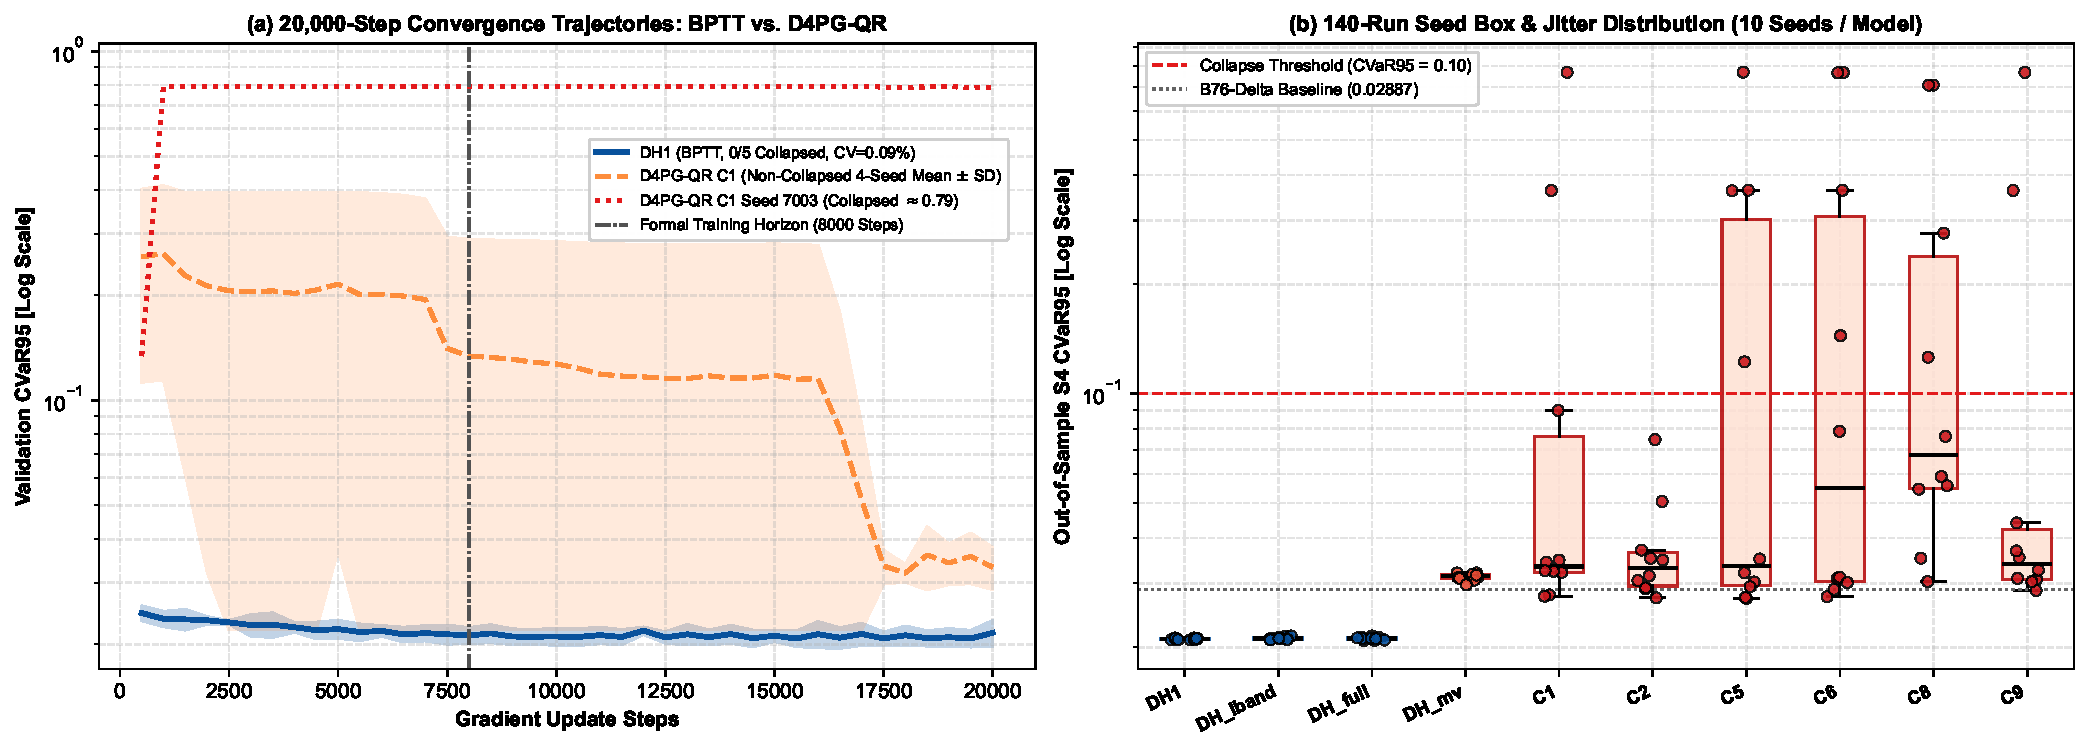
\includegraphics[width=\textwidth]{figures_en/Fig5_DH_vs_D4PG_QR_Stability_and_Collapse_EN.pdf}
  \caption{Optimization stability and convergence audit: (a) real $20,000$-step log-scale validation $\text{CVaR}_{95}$ convergence trajectories with $\pm 1\text{ SD}$ shaded ribbons comparing \texttt{DH1} against \texttt{D4PG-QR (C1)}; (b) 140-run box-and-jittered individual seed distribution plot (log scale, $10$ seeds per configuration) across \texttt{DH} and \texttt{D4PG-QR (C1--C9)}.}
  \label{fig:fig5}
\end{figure}

\subsection{Zero-Shot Out-of-Distribution (OOD) Generalization on the S5 Extreme Stress Benchmark ($20,000$ Paths)}
\label{sec:s5_stress}
To test whether policies trained in the baseline S4 market generalize without retraining to an unseen crisis regime, we evaluate all 80 S4-trained \texttt{DH} checkpoints directly on the frozen \textbf{S5 extreme stress benchmark} (\texttt{S5\_test.npz}, $N = 20,000$ paths; branching ratio doubled to $n = 0.6$, tight uniform limit ratio $\ell = 0.07$, jump size scaled by $\times 1.5$). On \texttt{S5\_test.npz}, pathwise jump incidence is $65.80\%$ ($13,159$ paths), while the price-limit hit path incidence more than doubles from $16.51\%$ (S4) to $35.77\%$ ($7,153$ limit-hit paths) and the locked-path incidence more than triples from $3.00\%$ (S4) to $10.08\%$ ($2,016$ locked paths).

\begin{table}[htbp]
  \centering
  \caption{Zero-shot out-of-distribution hedging performance on the S5 extreme stress benchmark ($20,000$ paths, $10$ seeds \texttt{9001--9010}, $n=0.6$, $\ell=0.07$, jump scale $\times 1.5$).}
  \label{tab:s5_stress}
  \resizebox{\textwidth}{!}{%
  \begin{tabular}{lcccccccccc}
    \toprule
    Policy / Configuration & S5 $\text{CVaR}_{95}$ (Mean $\pm$ SD) & S5 $\text{VaR}_{95}$ & S5 $\text{CVaR}_{99}$ & Cost ($\times 10^{-3}$) & Turnover & Trade Freq. & S5 Lock Gap ($\times 10^{-2}$) & Cond.\ $\text{CVaR}_{95}$ (Hit-Sub, $N=7,153$) & Cond.\ $\text{CVaR}_{95}$ (Lock-Sub, $N=2,016$) & Gain vs.\ \texttt{B76-Delta} \\
    \midrule
    \texttt{No-Hedge} & $0.313807$ & $0.213785$ & $0.479130$ & $0.0000$ & $0.0000$ & $0.00\%$ & $0.000$ & $0.386006$ & $0.412910$ & --- \\
    \texttt{B76-Delta} & $0.032554$ & $0.019401$ & $0.055556$ & $0.3235$ & $3.1740$ & $97.06\%$ & $1.791$ & $0.046937$ & $0.064158$ & Reference ($0.00\%$) \\
    \texttt{Leland-Delta} & $0.032543$ & $0.019387$ & $0.055488$ & $0.3231$ & $3.1699$ & $97.09\%$ & $1.788$ & $0.046889$ & $0.064073$ & $+0.03\%$ \\
    \texttt{WW-Band} ($\gamma_{\text{WW}}=0.25$) & $0.035753$ & $0.021957$ & $0.059813$ & $0.2353$ & $2.2918$ & $62.40\%$ & $1.628$ & $0.050855$ & $0.068554$ & $-9.83\%$ (Worse) \\
    \texttt{WW-Band} ($\gamma_{\text{WW}}=1.0$) & $0.047616$ & $0.030716$ & $0.075366$ & $0.1697$ & $1.6326$ & $35.06\%$ & $1.151$ & $0.065188$ & $0.085010$ & $-46.27\%$ (Worse) \\
    \midrule
    \texttt{DH\_mv} & $0.026697 \pm 0.001292$ & $0.012344$ & $0.053374$ & $0.4772$ & $4.7932$ & $99.82\%$ & $3.310$ & $0.042558$ & $0.062508$ & $+17.99\%$ \\
    \texttt{DH\_nolam} & $0.020550 \pm 0.000255$ & $0.012337$ & $\mathbf{0.038791}$ & $0.3067$ & $3.0131$ & $99.82\%$ & $2.139$ & $\mathbf{0.030915}$ & $\mathbf{0.046929}$ & $+36.87\%$ \\
    \texttt{DH1} & $0.020395 \pm 0.000412$ & $0.011983$ & $0.039100$ & $0.3081$ & $3.0273$ & $99.82\%$ & $2.162$ & $0.031085$ & $0.047454$ & $+37.35\%$ \\
    \texttt{DH\_oracle} & $0.020756 \pm 0.000427$ & $0.012107$ & $0.039620$ & $0.3078$ & $3.0210$ & $99.81\%$ & $2.146$ & $0.031584$ & $0.047893$ & $+36.24\%$ \\
    \texttt{DH\_cband} & $0.020879 \pm 0.000388$ & $0.012179$ & $0.039275$ & $\mathbf{0.2523}$ & $\mathbf{2.4688}$ & $\mathbf{56.01\%}$ & $2.156$ & $0.031567$ & $0.047578$ & $+35.86\%$ \\
    \textbf{\texttt{DH\_lband}} & $0.020711 \pm 0.000467$ & $0.012175$ & $0.039132$ & $\mathbf{0.2810}$ & $\mathbf{2.7613}$ & $\mathbf{78.74\%}$ & $2.146$ & $0.031366$ & $\mathbf{0.047280}$ & $+36.38\%$ \\
    \texttt{DH\_limit} & $0.020465 \pm 0.000315$ & $0.011836$ & $0.039532$ & $0.3100$ & $3.0436$ & $99.81\%$ & $3.028$ & $0.031355$ & $0.047724$ & $+37.13\%$ \\
    \textbf{\texttt{DH\_full} (Full Model)} & $\mathbf{0.020314 \pm 0.000382}$ & $\mathbf{0.011820}$ & $0.039122$ & $0.2882$ & $2.8238$ & $\mathbf{79.70\%}$ & $\mathbf{1.607}$ & $0.031084$ & $0.047368$ & $\mathbf{+37.60\%\ (\text{Best})}$ \\
    \bottomrule
  \end{tabular}%
  }
  \vspace{3pt}\par\noindent
  \begin{minipage}{\textwidth}
    \footnotesize
    \textit{Notes:} All S4-trained checkpoints ($M = 10$ seeds \texttt{9001--9010}, \texttt{ddof=1}) are evaluated zero-shot on \texttt{S5\_test.npz} ($N = 20,000$ paths, $P_0 = 0.064603$, $\sigma_{\text{imp}} = 0.020756\text{ day}^{-1/2}$; path-block bootstrap $\text{SE}_{\text{path}} \approx 0.00042$). \texttt{Cond.\ CVaR95 (Hit-Sub)} and \texttt{Cond.\ CVaR95 (Lock-Sub)} denote the conditional $95\%$ CVaR computed within the $N = 7,153$ limit-hit paths (tail size $358$) and $N = 2,016$ limit-locked paths (tail size $101$), respectively. For \texttt{DH1} and \texttt{DH\_full}, unconditional S5 $\text{Mean}(L)$ is $-0.007200$ and $-0.007292$, so the drift-neutralized tail risk $\widetilde{\text{CVaR}}_{95} = \text{CVaR}_{95} - \text{Mean}(L)$ is $0.027595$ ($+18.01\%$ above S4's $0.023384$) and $0.027606$ ($+17.89\%$ above S4's $0.023417$), respectively.
  \end{minipage}
\end{table}

Table~\ref{tab:s5_stress} and Figure~\ref{fig:fig6} highlight three crisis-generalization findings:
\begin{enumerate}
  \item \textbf{Amplified Tail-Risk Reduction Under Intensified Limit Hits:} While \texttt{B76-Delta} degrades from $\text{CVaR}_{95} = 0.028872$ in S4 to $0.032554$ in S5 (and asymptotic \texttt{WW-Band} deteriorates even more severely to $0.035753$ at $\gamma_{\text{WW}}=0.25$ and $0.047616$ at $\gamma_{\text{WW}}=1.0$), our full microstructure-aware policy \texttt{DH\_full} achieves the lowest overall $\text{CVaR}_{95} = 0.020314 \pm 0.000382$ across all models---expanding its relative improvement over \texttt{B76-Delta} from $27.00\%$ in S4 to $37.60\%$ in S5. On the $2,016$ limit-locked paths (\texttt{Lock-Sub}), \texttt{DH\_full} ($0.047368$) and \texttt{DH\_lband} ($0.047280$) cut conditional tail loss by $26.17\%$ and $26.31\%$ relative to \texttt{B76-Delta} ($0.064158$).
  \item \textbf{Decomposing Raw $\text{CVaR}_{95}$ vs.\ Drift-Neutralized Tail Risk $\widetilde{\text{CVaR}}_{95}$ Across S4 and S5:} Why is raw uncentered neural $\text{CVaR}_{95}$ slightly lower in S5 ($0.020314\text{--}0.020879$) than in S4 ($0.021021\text{--}0.021512$)? As shown in Equation~(\ref{eq:loss_expectation}), because $P_0 = \widehat{\mathbb{E}}[V_T]$ cancels in expectation ($\mathbb{E}[L_T] = -\mathbb{E}[G_T^{\text{fut}}]/F_0 + \mathbb{E}[C_T^{\text{fut}}]/F_0$), a higher $P_0$ does not by itself create a wealth cushion; rather, S5 combines $1.5\times$ larger left-skewed Kou jumps with a tighter symmetric price limit ($\ell = 0.07$ vs.\ $\bar{\ell} \approx 0.093$ in S4), which censors extreme downward jumps more heavily than upward jumps ($\widehat{\mathbb{E}}[F_T] = 1.0162$ in S5 vs.\ $1.0029$ in S4). Consequently, a long delta hedge ($\bar{\delta} \approx 0.55$) earns a larger expected futures gain $\mathbb{E}[G_T^{\text{fut}}]/F_0$, shifting unconditional $\text{Mean}(L)$ from $-0.002306$ (S4) to $-0.007200$ (S5) by $\Delta\text{Mean}(L) = -0.004894$, while the tighter $\ell = 0.07$ cap also bounds single-day moves on the $86.9\%$ of realized S5 limit-hit days that do not lock (matching the theoretical $1 - p_{\text{lock}} = 6/7 \approx 85.71\%$ unlocked rate). When we subtract $\text{Mean}(L)$ to isolate pure centered dispersion, the **drift-neutralized tail risk** $\widetilde{\text{CVaR}}_{95} = \text{CVaR}_{95} - \text{Mean}(L)$ strictly **increases by $+18.01\%$ from S4 ($0.023384$) to S5 ($0.027595$)** for \texttt{DH1} and by **$+17.89\%$ ($0.023417 \to 0.027606$)** for \texttt{DH\_full}, alongside a rise in raw $\text{CVaR}_{99}$ from $0.036892$ (S4) to $0.039122$ (S5).
  \item \textbf{Joint Microstructure Protection (\texttt{DH\_full} and \texttt{DH\_lband}):} Under the more than doubled limit-hit incidence of S5, \texttt{DH\_full} reduces the cumulative unexecuted lock-step hedging gap (\texttt{LockGap}) by $25.67\%$ relative to \texttt{DH1} ($1.607 \times 10^{-2}$ vs.\ $2.162 \times 10^{-2}$) and by $10.24\%$ relative to \texttt{B76-Delta} ($1.791 \times 10^{-2}$), while reducing trading frequency to $79.70\%$ and saving $6.46\%$ in transaction costs ($0.2882 \times 10^{-3}$ vs.\ $0.3081 \times 10^{-3}$). Meanwhile, \texttt{DH\_lband} cuts transaction costs by $8.80\%$ ($0.2810 \times 10^{-3}$ vs.\ $0.3081 \times 10^{-3}$) at a $78.74\%$ trading frequency.
\end{enumerate}

\begin{figure}[htbp]
  \centering
  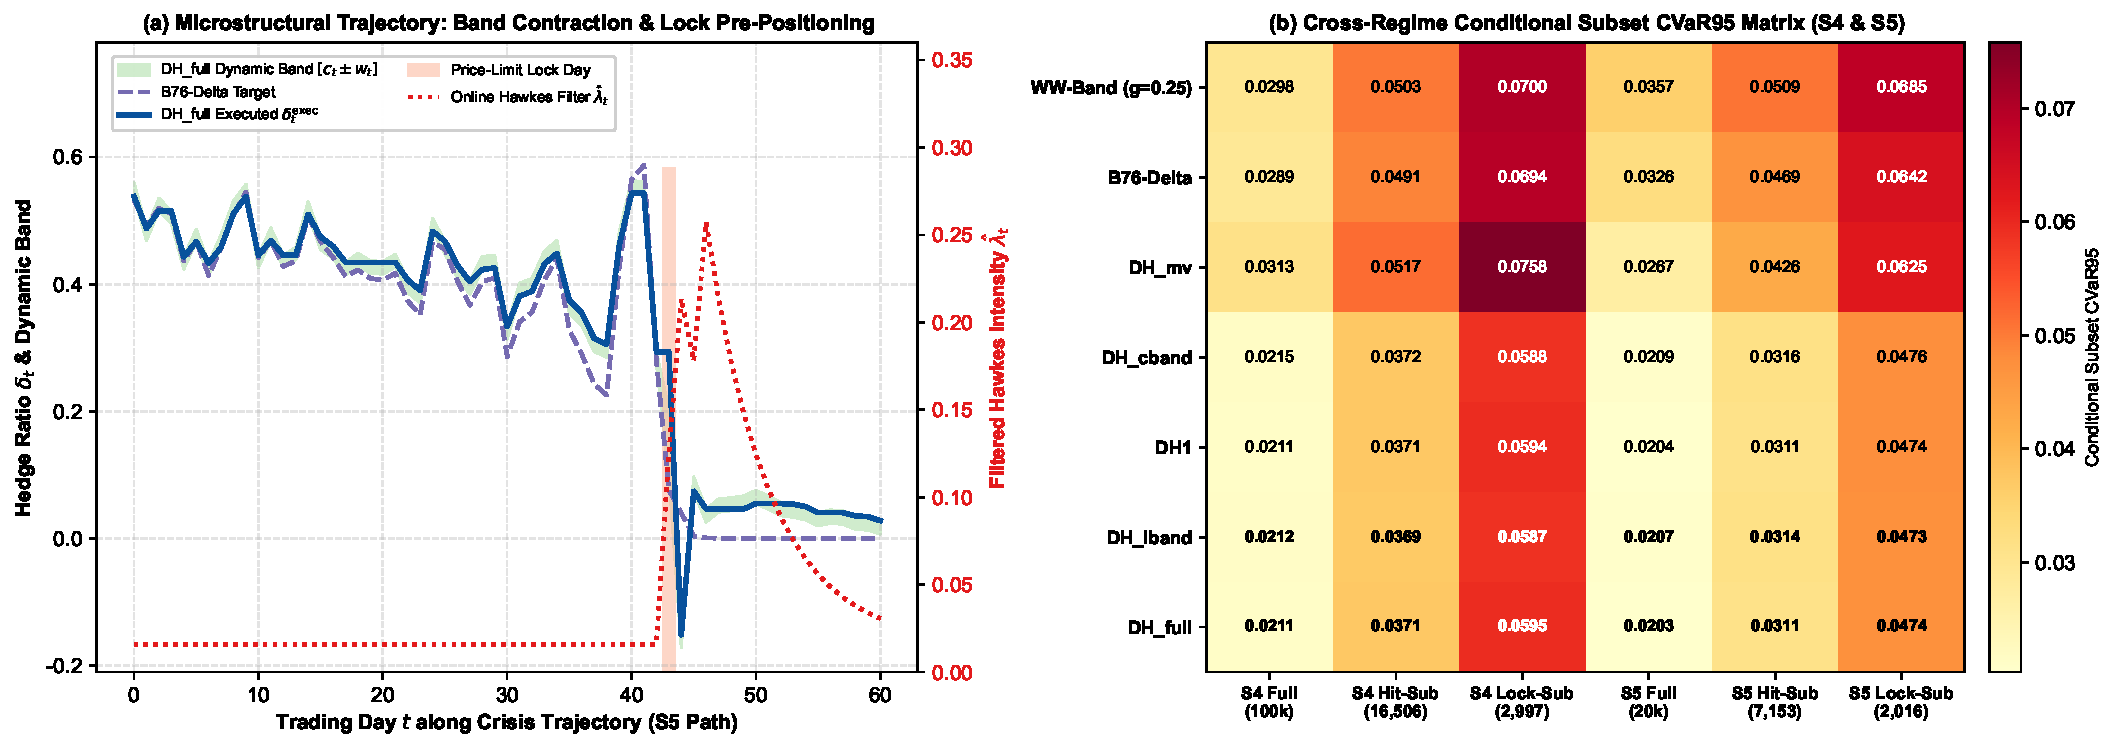
\includegraphics[width=\textwidth]{figures_en/Fig6_S5_OOD_Stress_and_CrossRegime_CVaR_EN.pdf}
  \caption{Out-of-distribution crisis generalization and microstructural trajectory tracking: (a) pathwise microstructural trajectory along a representative S5 crisis path showing the dynamic no-trade band $[c_t \pm w_t]$, executed hedge position $\delta_t^{\text{exec}}$ vs.\ \texttt{B76-Delta}, online Hawkes intensity $\hat{\lambda}_t$, and price-limit lock days; (b) 2D cross-regime conditional subset $\text{CVaR}_{95}$ matrix heatmap across S4 ($100,000$ full, $16,506$ hit, $2,997$ lock) and S5 ($20,000$ full, $7,153$ hit, $2,016$ lock) subsets.}
  \label{fig:fig6}
\end{figure}

% ==============================================================================
% SECTION 5: DISCUSSION, LIMITATIONS, AND CONCLUSION
% ==============================================================================
\section{Discussion, Limitations, and Conclusion}
\label{sec:discussion}

\subsection{Discussion: Microstructural Mechanisms, Architectural Channels, and Practical Implications}
Our multi-model audit across $80$ 1D Deep Hedging (\texttt{DH}) checkpoints, $60$ Distributional Actor-Critic (\texttt{D4PG-QR}) runs, and $80$ 2D Option-Gamma checkpoints (\texttt{TorchHedgeEnvOpt}) resolves a central question in the empirical deep hedging literature \citep{Mikkila2023,Francois2025} and non-Markovian volatility hedging \citep{Horvath2021,AbiJaber2025}: \emph{when, why, and through which architectural channel do explicit jump-intensity signals and institutional microstructure features improve derivative hedging?}

\paragraph{1. The Instrument-Spanning and Architectural Condition for Jump-Intensity Signals ($\mathbf{H_0, H_1}$).}
In a single-instrument futures hedging setting ($\Gamma^{\text{fut}} = 0$), feeding either the causal Hawkes filter $\hat{\lambda}_t$ (\texttt{DH1}, $\text{CVaR}_{95} = 0.021078$) or the unobservable true intensity $\lambda_t$ (\texttt{DH\_oracle}, $\text{CVaR}_{95} = 0.021085$) into an unconstrained MLP policy yields no aggregate $\text{CVaR}_{95}$ improvement over the jump-blind policy \texttt{DH\_nolam} ($0.021073$). Our Jacobian saliency audit (Table~\ref{tab:saliency}) shows that this invariance arises because linear futures cannot span quadratic jump-convexity losses $-\frac{1}{2}\Gamma_{\text{B76},t}(\Delta F_t)^2$ \emph{ex ante} when jump signs are two-sided ($p_{\text{up}} = 0.4$). Introducing a rolling $\tau_h = 20$-day ATM call option $\eta_t$ in \texttt{TorchHedgeEnvOpt} (Table~\ref{tab:plan_a}) breaks this spanning ceiling across all 2D policies ($\text{CVaR}_{95}$ reduced by $17.98\%\text{--}29.95\%$ relative to 1D counterparts) \citep{CarbonneauGodin2024}. Crucially, our 10-seed audit reveals a sharp separation between unconstrained and structurally constrained uses of $\hat{\lambda}_t$: feeding $\hat{\lambda}_t$ directly into an unconstrained 2D MLP (\texttt{DH\_opt1}, $0.015226 \pm 0.001497$) lowers 10-seed point $\text{CVaR}_{95}$ by $+11.91\%$ relative to \texttt{DH\_opt\_nolam} ($0.017284 \pm 0.004298$, $p_{\text{holm}} = 0.450$; $+21.56\%$ in the 5-seed subset) and largely overlaps with nonlinear EWMA volatility features (\texttt{DH\_opt\_ewma\_nl}, $0.015904 \pm 0.001742$), whereas channeling $\hat{\lambda}_t$ through the multiplicative no-trade band (\texttt{DH\_opt\_lband}) achieves the lowest realistic 2D tail risk of $0.014841 \pm 0.001316$, outperforming static-band \texttt{DH\_opt\_cband} ($0.017546 \pm 0.002298$) by $+15.41\%$ ($t = -7.401, p_{\text{holm}} = 0.000123$). Thus, extracting statistically reliable gains from jump-intensity filtering requires both a convex hedging instrument and a structural band parameterization that regularizes non-convex optimization variance.

\paragraph{2. Endogenous Microstructural Adaptation in Jump-Modulated No-Trade Bands ($\mathbf{H_1}$).}
Across both 1D and 2D markets, channeling $\hat{\lambda}_t$ into the multiplicative no-trade band width $w_t(x_t) = \text{softplus}(g_\phi(x_{t,-\lambda}))\exp(\theta\hat{\lambda}_t)$ (\texttt{DH\_lband}, \texttt{DH\_full}, and \texttt{DH\_opt\_lband}, extending neural band networks \citealt{Imaki2023,Luetkebohmert2022}) produces a consistent microstructural adaptation. Across 10 random seeds, gradient optimization without sign constraints learns a negative slope $\hat{\theta} = -0.0276 \pm 0.0202$ ($p = 0.0019$) in 1D \texttt{DH\_lband}, $\hat{\theta} = -0.0230 \pm 0.0153$ ($p = 0.0011$) in 1D \texttt{DH\_full}, and $\hat{\theta} = -0.0290 \pm 0.0064$ ($p = 1.59 \times 10^{-7}$) in 2D \texttt{DH\_opt\_lband}. By contracting the no-trade band during jump-clustering bursts and widening it during tranquil periods, 1D \texttt{DH\_lband} outperforms the static band \texttt{DH\_cband} on S4 ($p_{\text{holm}} = 0.00063$), saves $8.09\%$ in transaction costs and $20.11\%$ in trading frequency relative to \texttt{DH1} (at the cost of a $+0.52\%$ higher $\text{CVaR}_{95}$ at $1\times$ fee where cost savings are smaller than band tracking error), and achieves non-inferior tail risk to unconstrained \texttt{DH1} under $6\times$ transaction costs ($0.023145$ vs.\ $0.023241$, two-sided $p = 0.218$, TOST equivalence $p_{\text{TOST}} = 0.046 < 0.05$ within $\pm 1.0\%$) while saving $8.11\%$ in friction (Table~\ref{tab:plan_a} Panel~B).

\paragraph{3. Asymmetric Tail Optimization ($\mathbf{H_2}$) and End-to-End BPTT Stability.}
Across the tested risk-aversion range $\lambda_{\text{MV}} \in [0.5, 50.0]$ (Table~\ref{tab:mv_sweep}), symmetric mean-variance hedging (\texttt{DH\_mv}) reaches an empirical $\text{CVaR}_{95}$ lower bound of $0.027332$ ($29.67\%$ higher than \texttt{DH1}, corresponding to a $22.88\%$ relative reduction achieved by \texttt{DH1}) because quadratic variance penalizes upside convex windfalls ($L_T < 0$) identically to downside tail losses ($L_T > 0$), inflating turnover to $4.0981\text{--}5.0256$; consequently, \texttt{DH1} strictly dominates \texttt{DH\_mv} in the $(\text{CVaR}_{95}, \text{Cost})$ plane while trading off a slightly higher symmetric $\text{Std}(L)$ ($0.013391$ vs.\ $0.012539\text{--}0.012798$). In addition, our 140-run optimization audit (Table~\ref{tab:stability}) shows that in a finite-horizon ($T = 60$) environment with piecewise-differentiable dynamics, direct pathwise BPTT (\texttt{DH}) achieves a $0\%$ seed collapse rate and a $0.50\%$ cross-seed coefficient of variation, whereas model-free distributional reinforcement learning (\texttt{D4PG-QR}, \citealt{Cao2023,ChenHu2026}) suffers a $20\%\text{--}30\%$ seed collapse rate when exposed to spiky Hawkes jump signals (\texttt{C1} vs.\ \texttt{C2}) and price-limit truncations.

\paragraph{4. Practical and Regulatory Implications for Commodity Hedging Desks and Exchanges.}
For industrial risk managers and derivative market makers in strategic battery metals \citep{Kong2024,Geng2025}, our findings offer three conditional guidelines grounded in our empirical trade-offs. First, when hedging solely with linear futures at low exchange fee tiers ($c = 10^{-4}$), desks must weigh the $+0.52\%$ aggregate $\text{CVaR}_{95}$ tracking-error trade-off of jump-modulated bands against their microstructural execution benefits: deploying \texttt{DH\_lband} and price-limit state features (\texttt{DH\_full}) is warranted when execution desks prioritize cutting turnover costs by $6\%\text{--}8\%$, compressing unexecuted lock-day hedging gaps by $26\%\text{--}30\%$, or operating under elevated ($6\times$) slippage tiers, rather than expecting linear delta shifts to eliminate jump-Gamma risk. Second, to materially reduce aggregate tail shortfall ($\text{CVaR}_{95}$), hedgers must augment futures with short-dated options and channel jump-intensity forecasts into structural band modulation (\texttt{DH\_opt\_lband}), monitoring implied-volatility spike elasticity ($\kappa_{\text{iv}}$) so option purchases are not executed at excessive volatility risk premiums. Third, for commodity exchanges such as GFEX---which listed Lithium Carbonate (\texttt{LC}) options alongside futures on July 24, 2023---our results demonstrate that deepening market-making liquidity in short-dated commodity options across strike tiers is essential for completing the market and mitigating the unhedgeable Gamma exposure faced by commercial liquidity providers during limit-lock episodes.

\subsection{Empirically Observed Limitations}
\label{sec:limitations}
Six concrete empirical limitations emerge from our experiments. First, while diffusive volatility ($\sigma = 0.016144$), empirical price-limit tiers ($\ell \in [0.07, 0.15]$), conditional lock probability ($p_{\text{lock}} = 1/7 \approx 0.1429$), and post-jump drift half-life ($\beta = 0.20\text{ day}^{-1}$ from $h = 1\text{--}4$ day continuation $t = 2.09\text{--}3.47$) are anchored to 542 trading days of GFEX Lithium Carbonate (\texttt{LC}) futures (\texttt{2023-07-24} to \texttt{2025-10-20}), that window contains only $7$ limit-hit days ($1.29\%$), $1$ full-day lock ($0.185\%$), and $10$ tail events exceeding $3\sigma$, so $(n, \bar{\lambda}) = (0.3, 0.04)$ and $(p_{\text{up}}, \eta_{\text{up}}, \eta_{\text{dn}}) = (0.4, 40.0, 25.0)$ are fixed as protocol-specified scenario values rather than joint maximum-likelihood estimates; because all evaluations are conducted in a semi-synthetic simulator partially calibrated to GFEX \texttt{LC} futures rather than on empirical option market prices, the external validity of our conclusions has not been tested on real market data. Second, our causal threshold filter $\hat{I}_t = \mathbb{I}(|r_t| > 3\sigma \lor \text{limit\_hit}_t = 1)$ misses moderate jumps with $|J| < 3\sigma = 0.0484$, resulting in a true-positive recall of $13.78\%$ on \texttt{TH2b} ($\text{TP}=4,138, \text{FP}=1,757$, precision $70.20\%$, raw detection ratio $19.63\%$, bias $-45.17\%$) and $18.63\%$ on \texttt{S4\_test.npz} ($\text{TP}=44,052, \text{FP}=4,831$, precision $90.12\%$, $r = 0.4455$, bias $-24.44\%$). Third, when hedging solely with linear futures at baseline cost $c = 10^{-4}$, aggregate $\text{CVaR}_{95}$ across all CVaR policies is compressed within $0.021021\text{--}0.021187$, and \texttt{DH\_lband} ($0.021187$) incurs a $0.52\%$ higher $\text{CVaR}_{95}$ than unconstrained \texttt{DH1} ($0.021078$) because $1\times$ fee savings ($2.56 \times 10^{-5}$) are smaller than band tracking error, requiring $6\times$ transaction costs ($0.023145$ vs.\ $0.023241$, two-sided $p = 0.218$, $p_{\text{TOST}} = 0.046$) or a 2D option leg to eliminate this penalty. Fourth, in the 10-seed 2D option-hedging benchmark, feeding $\hat{\lambda}_t$ into an unconstrained MLP (\texttt{DH\_opt1}, $0.015226 \pm 0.001497$) yields an $11.91\%$ point reduction over \texttt{DH\_opt\_nolam} ($0.017284 \pm 0.004298$, $p_{\text{holm}} = 0.450$, $\text{MDE}_{80\%} = 28.76\%$) that does not achieve standalone statistical significance due to cross-seed optimization variance and collinearity with nonlinear $\sigma_{\text{EWMA}}$ features (\texttt{DH\_opt\_ewma\_nl}, $0.015904$), and this unconstrained gain attenuates from $+11.91\%$ ($\kappa_{\text{iv}}=0$) to $+5.31\%$ ($\kappa_{\text{iv}}=2$) and $+0.73\%$ ($\kappa_{\text{iv}}=5$) under dynamic implied-volatility spikes, so our 2D percentage gains do not constitute estimates of realizable trading profits. Fifth, off-policy \texttt{D4PG-QR} (\texttt{C1--C9}) exhibits a $20\%\text{--}30\%$ seed collapse rate ($\text{CVaR}_{95} > 0.10$) whenever jump or limit signals are included, with non-collapsed \texttt{D4PG-QR (C1)} seeds averaging $0.038934 \pm 0.020739$ and degrading further at $20,000$ updates. Sixth, while each trajectory's limit ratio $\ell$ is drawn from the empirical GFEX distribution ($7\%\text{--}15\%$), $\ell$ is held constant within each 60-day path rather than modeling dynamic consecutive-day exchange limit adjustments.

\subsection{Conclusion}
\label{sec:conclusion}
In our semi-synthetic numerical setting partially calibrated to Guangzhou Futures Exchange Lithium Carbonate (\texttt{LC}) futures, we conducted a multi-model empirical and microstructural audit of Deep Hedging under self-exciting Hawkes jump clustering and institutional price-limit locks. Our findings support four principal conclusions:
\begin{enumerate}
  \item \textbf{Asymmetric Tail Risk Optimization:} Across all tested market regimes and risk-aversion parameters, training with the Rockafellar-Uryasev $\text{CVaR}_{95}$ objective outperforms both classical analytical baselines (\texttt{B76-Delta}, \texttt{Leland-Delta}, \texttt{WW-Band}) and symmetric mean-variance neural policies (\texttt{DH\_mv}) in the $(\text{CVaR}_{95}, \text{Cost})$ plane, avoiding the empirical tail-risk lower bound and excessive turnover induced by symmetric variance penalties.
  \item \textbf{Microstructural Adaptation via Jump-Modulated No-Trade Bands and Limit Features:} Embedding the causal online Hawkes intensity $\hat{\lambda}_t$ into a multiplicative no-trade band (\texttt{DH\_lband}, \texttt{DH\_full}, and \texttt{DH\_opt\_lband}) leads the network to consistently learn a negative modulation slope ($\hat{\theta} < 0$), narrowing the no-trade buffer during jump-clustering bursts and widening it during calm periods. In the single-instrument setting, this mechanism reduces trading frequency and transaction costs while achieving the lowest $\text{CVaR}_{99}$ and conditional locked-subset $\text{CVaR}_{95}$, achieves non-inferior tail risk to unconstrained \texttt{DH1} under elevated transaction costs while cutting friction, and---when combined with price-limit features in \texttt{DH\_full}---compresses the cumulative unexecuted lock-step hedging gap (\texttt{LockGap}) across both the S4 benchmark and zero-shot generalization to the S5 extreme stress regime.
  \item \textbf{Option-Gamma Spanning and Structural Band Parameterization as the Dual Keys for Jump Filtering:} Input Jacobian saliency diagnostics, nonlinear EWMA controls, and oracle-intensity experiments demonstrate that linear futures alone cannot hedge \emph{ex-ante} quadratic jump-Gamma risk. Extending the action space to include a rolling short-dated ATM call option (\texttt{TorchHedgeEnvOpt}) breaks the single-instrument spanning ceiling across all policies, and channeling $\hat{\lambda}_t$ through the multiplicative no-trade band (\texttt{DH\_opt\_lband}) overcomes the cross-seed optimization variance and EWMA collinearity of unconstrained MLPs to deliver a statistically significant and economically large tail-risk reduction.
  \item \textbf{Algorithmic Advantage of Direct BPTT over Off-Policy Distributional RL:} When the accounting and microstructural execution rules are known and piecewise differentiable, end-to-end BPTT (\texttt{DH}) provides zero seed collapse and sub-$1\%$ cross-seed variation, outperforming off-policy quantile actor-critic (\texttt{D4PG-QR}) across all training budgets.
\end{enumerate}

\section*{Code and Data Availability}
All simulation environments (\texttt{src/simulator.py}, \texttt{src/torch\_env.py}, \texttt{src/torch\_env\_opt.py}), neural network architectures (\texttt{src/networks.py}), training pipelines (\texttt{src/trainer.py}), experiment configuration protocols (\texttt{configs/experiment\_protocol.json}), archived summary statistics (\texttt{results/archived\_summary\_tables.json} and \texttt{results/tables\_csv/}), and automated consistency verification scripts (\texttt{src/verify\_archived\_tables.py}) supporting the findings of this study are openly available on GitHub at \url{https://github.com/lewygoat/Jump-Risk-Filtering-Deep-Hedging}.

\section*{Declaration of Competing Interest}
The authors declare that they have no known competing financial interests or personal relationships that could have appeared to influence the work reported in this paper.

\section*{Funding}
This research received no specific grant from any funding agency in the public, commercial, or not-for-profit sectors.

% ==============================================================================
% REFERENCES
% ==============================================================================
\begin{thebibliography}{99}

\bibitem[Abi Jaber and G\'{e}rard(2025)]{AbiJaber2025}
Abi Jaber, E., \& G\'{e}rard, L.-A. (2025).
Signature volatility models: pricing and hedging with Fourier.
\emph{arXiv preprint arXiv:2402.01820v2}.
\url{https://doi.org/10.48550/arXiv.2402.01820}

\bibitem[A\"{i}t-Sahalia et~al.(2015)]{AitSahalia2015}
A\"{i}t-Sahalia, Y., Cacho-Diaz, J., \& Laeven, R.~J.~A. (2015).
Modeling financial contagion using mutually exciting jump processes.
\emph{Journal of Financial Economics}, 117(3), 585--606.
\url{https://doi.org/10.1016/j.jfineco.2015.03.002}

\bibitem[Babaei(2024)]{Babaei2024}
Babaei, E. (2024).
Asset pricing and hedging in financial markets with fixed and proportional transaction costs.
\emph{Annals of Finance}, 20(2), 259--275.
\url{https://doi.org/10.1007/s10436-024-00441-w}

\bibitem[Bacry et~al.(2015)]{Bacry2015}
Bacry, E., Mastromatteo, I., \& Muzy, J.-F. (2015).
Hawkes processes in finance.
\emph{Market Microstructure and Liquidity}, 1(1), 1550005.
\url{https://doi.org/10.1142/S2382626615500057}

\bibitem[Bakshi et~al.(1997)]{Bakshi1997}
Bakshi, G., Cao, C., \& Chen, Z. (1997).
Empirical performance of alternative option pricing models.
\emph{The Journal of Finance}, 52(5), 2003--2049.
\url{https://doi.org/10.1111/j.1540-6261.1997.tb02749.x}

\bibitem[Black(1976)]{Black1976}
Black, F. (1976).
The pricing of commodity contracts.
\emph{Journal of Financial Economics}, 3(1--2), 167--179.
\url{https://doi.org/10.1016/0304-405X(76)90024-6}

\bibitem[Boyle and Emanuel(1980)]{BoyleEmanuel1980}
Boyle, P.~P., \& Emanuel, D. (1980).
Discretely adjusted option hedges.
\emph{Journal of Financial Economics}, 8(3), 259--282.
\url{https://doi.org/10.1016/0304-405X(80)90003-3}

\bibitem[Brignone et~al.(2023)]{Brignone2023}
Brignone, R., Gonzato, L., \& Sgarra, C. (2023).
Commodity Asian option pricing and simulation in a 4-factor model with jump clusters.
\emph{Annals of Operations Research}, 336(1--2), 275--306.
\url{https://doi.org/10.1007/s10479-022-05152-x}

\bibitem[Brugi\`{e}re and Turinici(2026)]{Brugiere2026}
Brugi\`{e}re, P., \& Turinici, G. (2026).
Model-free deep hedging with transaction costs and light and augmented data methods.
\emph{The Journal of Derivatives}, 33(4), 27--53.
\url{https://doi.org/10.3905/jod.2026.004}

\bibitem[Buehler et~al.(2019)]{Buehler2019}
Buehler, H., Gonon, L., Teichmann, J., \& Wood, B. (2019).
Deep hedging.
\emph{Quantitative Finance}, 19(8), 1271--1291.
\url{https://doi.org/10.1080/14697688.2019.1571683}

\bibitem[Cao et~al.(2023)]{Cao2023}
Cao, J., Chen, J., Farghadani, S., Hull, J., Poulos, Z., Wang, Z., \& Yuan, J. (2023).
Gamma and vega hedging using deep distributional reinforcement learning.
\emph{Frontiers in Artificial Intelligence}, 6, 1129370.
\url{https://doi.org/10.3389/frai.2023.1129370}

\bibitem[Carbonneau(2021)]{Carbonneau2021}
Carbonneau, A. (2021).
Deep hedging of long-term financial derivatives.
\emph{Insurance: Mathematics and Economics}, 99, 327--340.
\url{https://doi.org/10.1016/j.insmatheco.2021.03.017}

\bibitem[Carbonneau and Godin(2024)]{CarbonneauGodin2024}
Carbonneau, A., \& Godin, F. (2024).
Deep equal risk pricing of illiquid derivatives with multiple hedging instruments.
\emph{The Journal of Computational Finance}, 28(1), 1--36.
\url{https://doi.org/10.21314/jcf.2024.012}

\bibitem[Chen et~al.(2024)]{ChenClements2024}
Chen, J., Clements, M.~P., \& Urquhart, A. (2024).
Modeling price and variance jump clustering using the marked Hawkes process.
\emph{Journal of Financial Econometrics}, 22(3), 743--772.
\url{https://doi.org/10.1093/jjfinec/nbad007}

\bibitem[Chen et~al.(2026)]{ChenHu2026}
Chen, Z., Hu, M., Yi, J., \& Sun, W. (2026).
Reinforcement learning for option hedging: Static implied-volatility fit versus shortfall-aware performance.
\emph{Finance Research Letters}, 108, 110402.
\url{https://doi.org/10.1016/j.frl.2026.110402}

\bibitem[Coskun(2023)]{Coskun2023}
Coskun, M. (2023).
Dynamic correlations and volatility spillovers between subsectoral clean-energy stocks and commodity futures markets: A hedging perspective.
\emph{Journal of Futures Markets}, 43(12), 1727--1749.
\url{https://doi.org/10.1002/fut.22454}

\bibitem[Dabney et~al.(2018)]{Dabney2018}
Dabney, W., Rowland, M., Bellemare, M.~G., \& Munos, R. (2018).
Distributional reinforcement learning with quantile regression.
In \emph{Proceedings of the AAAI Conference on Artificial Intelligence}, 32(1), 2892--2901.
\url{https://doi.org/10.1609/aaai.v32i1.11791}

\bibitem[Dai et~al.(2022)]{Dai2022}
Dai, Z., Li, L., \& Zhang, G. (2022).
Evaluation of deep learning algorithms for quadratic hedging.
\emph{The Journal of Derivatives}, 30(1), 32--57.
\url{https://doi.org/10.3905/jod.2022.1.165}

\bibitem[de~Truchis et~al.(2025)]{deTruchis2025}
de~Truchis, G., Desgraupes, B., \& Dumitrescu, E.-I. (2025).
Assessing volatility persistence in fractional Heston models with self-exciting jumps.
\emph{Econometric Reviews}, 44(3), 275--311.
\url{https://doi.org/10.1080/07474938.2024.2409475}

\bibitem[Fran\c{c}ois et~al.(2025)]{Francois2025}
Fran\c{c}ois, P., Gauthier, G., Godin, F., \& Mendoza, C.~O.~P. (2025).
Is the difference between deep hedging and delta hedging a statistical arbitrage?
\emph{Finance Research Letters}, 73, 106590.
\url{https://doi.org/10.1016/j.frl.2024.106590}

\bibitem[Geng(2025)]{Geng2025}
Geng, Q. (2025).
Is there a robust hedging method during the COVID-19 pandemic? Evidence from Chinese crude oil futures.
\emph{Energy Economics}, 144, 108329.
\url{https://doi.org/10.1016/j.eneco.2025.108329}

\bibitem[Gouden\`{e}ge et~al.(2023)]{Goudenege2023}
Gouden\`{e}ge, L., Molent, A., \& Zanette, A. (2023).
Backward hedging for American options with transaction costs.
\emph{arXiv preprint arXiv:2305.06805v2}.
\url{https://doi.org/10.48550/arXiv.2305.06805}

\bibitem[Hawkes(1971)]{Hawkes1971}
Hawkes, A.~G. (1971).
Spectra of some self-exciting and mutually exciting point processes.
\emph{Biometrika}, 58(1), 83--90.
\url{https://doi.org/10.1093/biomet/58.1.83}

\bibitem[He et~al.(2026a)]{He2026}
He, Y., Ning, P., \& Song, Y. (2026a).
Jump volatility forecasting for crude oil futures based on complex network and hybrid CNN--Transformer model.
\emph{Mathematics}, 14(2), 258.
\url{https://doi.org/10.3390/math14020258}

\bibitem[He et~al.(2026b)]{HeYan2026}
He, X.-J., Yan, D., \& Lin, S. (2026b).
A new analytical approach for pricing variance and volatility swaps: Incorporating liquidity and self-exciting jumps.
\emph{Journal of Futures Markets}, 46(9), 1555--1569.
\url{https://doi.org/10.1002/fut.70120}

\bibitem[Horvath et~al.(2021)]{Horvath2021}
Horvath, B., Teichmann, J., \& \v{Z}uri\v{c}, \v{Z}. (2021).
Deep hedging under rough volatility.
\emph{Risks}, 9(7), 138.
\url{https://doi.org/10.3390/risks9070138}

\bibitem[Imaki et~al.(2023)]{Imaki2023}
Imaki, S., Imajo, K., Ito, K., Minami, K., \& Nakagawa, K. (2023).
No-transaction band network: A neural network architecture for efficient deep hedging.
\emph{The Journal of Financial Data Science}, 5(2), 84--99.
\url{https://doi.org/10.3905/jfds.2023.1.125}

\bibitem[Jouini et~al.(2026)]{Jouini2026}
Jouini, W., Derbel, M., Panazan, O., \& Gheorghe, C. (2026).
Multifractal cross-market dependence and dynamic hedging under crisis regimes: Evidence from commodity--equity interactions.
\emph{Fractal and Fractional}, 10(1), 5.
\url{https://doi.org/10.3390/fractalfract10010005}

\bibitem[Kim and Rhee(1997)]{KimRhee1997}
Kim, K.~A., \& Rhee, S.~G. (1997).
Price limit performance: Evidence from the Tokyo Stock Exchange.
\emph{The Journal of Finance}, 52(2), 885--901.
\url{https://doi.org/10.1111/j.1540-6261.1997.tb04827.x}

\bibitem[Kong et~al.(2024)]{Kong2024}
Kong, W., Cheng, J., \& Xiao, J. (2024).
Market risk of lithium industry chain---Evidence from listed companies.
\emph{Energies}, 17(23), 6173.
\url{https://doi.org/10.3390/en17236173}

\bibitem[Kou(2002)]{Kou2002}
Kou, S.~G. (2002).
A jump-diffusion model for option pricing.
\emph{Management Science}, 48(8), 1086--1101.
\url{https://doi.org/10.1287/mnsc.48.8.1086.166}

\bibitem[Leland(1985)]{Leland1985}
Leland, H.~E. (1985).
Option pricing and replication with transactions costs.
\emph{The Journal of Finance}, 40(5), 1283--1301.
\url{https://doi.org/10.1111/j.1540-6261.1985.tb02383.x}

\bibitem[L\"{u}tkebohmert et~al.(2022)]{Luetkebohmert2022}
L\"{u}tkebohmert, E., Schmidt, T., \& Sester, J. (2022).
Robust deep hedging.
\emph{Quantitative Finance}, 22(8), 1465--1480.
\url{https://doi.org/10.1080/14697688.2022.2056073}

\bibitem[Marzban et~al.(2022)]{Marzban2022}
Marzban, S., Delage, E., \& Li, J.~Y. (2022).
Equal risk pricing and hedging of financial derivatives with convex risk measures.
\emph{Quantitative Finance}, 22(1), 47--73.
\url{https://doi.org/10.1080/14697688.2021.1993614}

\bibitem[Mercuri et~al.(2024)]{Mercuri2024}
Mercuri, L., Perchiazzo, A., \& Rroji, E. (2024).
Option pricing with a compound CARMA(p,q)-Hawkes.
\emph{arXiv preprint arXiv:2412.15172v1}.
\url{https://doi.org/10.48550/arXiv.2412.15172}

\bibitem[Merton(1976)]{Merton1976}
Merton, R.~C. (1976).
Option pricing when underlying stock returns are discontinuous.
\emph{Journal of Financial Economics}, 3(1--2), 125--144.
\url{https://doi.org/10.1016/0304-405X(76)90022-2}

\bibitem[Mikkil\"{a} and Kanniainen(2023)]{Mikkila2023}
Mikkil\"{a}, O., \& Kanniainen, J. (2023).
Empirical deep hedging.
\emph{Quantitative Finance}, 23(1), 111--122.
\url{https://doi.org/10.1080/14697688.2022.2136037}

\bibitem[Na and Wan(2023)]{NaWan2023}
Na, A.~S., \& Wan, J.~W.~L. (2023).
Efficient pricing and hedging of high-dimensional American options using deep recurrent networks.
\emph{Quantitative Finance}, 23(4), 631--651.
\url{https://doi.org/10.1080/14697688.2023.2167666}

\bibitem[Naqvi et~al.(2023)]{Naqvi2023}
Naqvi, B., Mirza, N., Umar, M., \& Rizvi, S.~K.~A. (2023).
Shanghai crude oil futures: Returns independence, volatility asymmetry, and hedging potential.
\emph{Energy Economics}, 128, 107110.
\url{https://doi.org/10.1016/j.eneco.2023.107110}

\bibitem[Pickard and Lawryshyn(2023)]{Pickard2023}
Pickard, R., \& Lawryshyn, Y. (2023).
Deep reinforcement learning for dynamic stock option hedging: A review.
\emph{Mathematics}, 11(24), 4943.
\url{https://doi.org/10.3390/math11244943}

\bibitem[Qiao et~al.(2025)]{Qiao2025}
Qiao, G., Cui, W., Zhou, Y., \& Liang, C. (2025).
Volatility of volatility and VIX forecasting: New evidence based on jumps, the short-term and long-term volatility.
\emph{Journal of Futures Markets}, 45(1), 23--46.
\url{https://doi.org/10.1002/fut.22553}

\bibitem[Rockafellar and Uryasev(2000)]{Rockafellar2000}
Rockafellar, R.~T., \& Uryasev, S. (2000).
Optimization of conditional value-at-risk.
\emph{Journal of Risk}, 2(3), 21--41.
\url{https://doi.org/10.21314/JOR.2000.038}

\bibitem[Shakeel et~al.(2026)]{Shakeel2026}
Shakeel, M.~R., Yadav, S., \& Ahmad, M. (2026).
Option pricing under regime-switching jump-diffusion dynamics with transaction costs: A neural SDE approach.
\emph{Review of Derivatives Research}, 29(1), 16.
\url{https://doi.org/10.1007/s11147-026-09238-7}

\bibitem[Wang et~al.(2025)]{Wang2025}
Wang, W., Liu, H., Jiang, L., \& Wang, L. (2025).
Prediction of lithium carbonate prices in China applying a VMD--SSA--LSTM combined model.
\emph{Mathematics}, 13(4), 613.
\url{https://doi.org/10.3390/math13040613}

\bibitem[Whalley and Wilmott(1997)]{Whalley1997}
Whalley, A.~E., \& Wilmott, P. (1997).
An asymptotic analysis of an optimal hedging model for option pricing with transaction costs.
\emph{Mathematical Finance}, 7(3), 307--324.
\url{https://doi.org/10.1111/1467-9965.00034}

\bibitem[Xia et~al.(2024)]{Xia2024}
Xia, W., Xiong, T., \& Li, M. (2024).
Can night trading reduce price volatility? Evidence from China's corn and corn starch futures markets.
\emph{Journal of Futures Markets}, 44(4), 585--604.
\url{https://doi.org/10.1002/fut.22483}

\bibitem[Zhang et~al.(2023)]{Zhang2023}
Zhang, D., She, W., Qu, F., \& He, C. (2023).
Asymmetric risk connectedness between crude oil and agricultural commodity futures in China before and after the COVID-19 pandemic: Evidence from high-frequency data.
\emph{Energies}, 16(16), 5898.
\url{https://doi.org/10.3390/en16165898}

\end{thebibliography}

\end{document}
